%========== Compiler Directives ==========
% !TeX program = lualatex                                   
% !TeX encoding = utf8
% !TeX spellcheck = english

%========== Document settings ==========
\documentclass[11pt,a4paper,twoside,openany]{report}
\setlength\textwidth{145mm}
\setlength\textheight{247mm}
\setlength\oddsidemargin{14.2mm}
\setlength\evensidemargin{0mm}
\setlength\topmargin{0mm}
\setlength\headsep{0mm}
\setlength\headheight{0mm}
\let\openright=\cleardoublepage

%========== Language settings ==========
\usepackage[main=british,czech]{babel}

%========== Packages =============
\usepackage{thesis-package}

%========== Date format ===============
\newdateformat{monthyeardate}{\monthname[\THEMONTH] \THEYEAR}

%========== Bibliography ==========
\addbibresource{bibliography.bib}

%========== Draft settings ==========
\usepackage{lipsum}

\makeindex[intoc]
\makenomenclature
\renewcommand{\nomname}{Glossary of Symbols}
\begin{document}

\pagenumbering{gobble}

%========== Title page ==========
% Suppress displaying the page number on the title page + count the following page as page 1 (not used)
\begin{titlepage}
    % Define a new command for horizontal lines, change thickness here
\newcommand{\HRule}{\rule{\linewidth}{0.5mm}}
\center

%========== Header ==========
\textsc{\LARGE Czech Technical University in Prague,\\Faculty of Electrical Engineering}\\[1.5cm]
\textsc{\Large Master's thesis}\\[0.5cm]

%========== Title ==========
\HRule\\[0.6cm]
{\huge\bfseries Dual Circularly Polarized Waveguide Antenna}\\[0.3cm] % Title of your document
\HRule\\[1.5cm]

%========== Authors ==========
\begin{minipage}{0.45\textwidth}
    \begin{flushleft}
        \large
        \textit{Author}\\
        M. \textsc{Šimák}\\
        \textsc{Department of Electromagnetic Field}
    \end{flushleft}
\end{minipage}
~
\begin{minipage}{0.45\textwidth}
    \begin{flushright}
        \large
        \textit{Supervisor}\\
        doc. Ing. P. \textsc{Hazdra}, Ph.D.\\
        \textsc{Department of Electromagnetic Field}
    \end{flushright}
\end{minipage}

%========== Logo ==========
% Position at 3/4 of the screen
\vfill\vfill\vfill
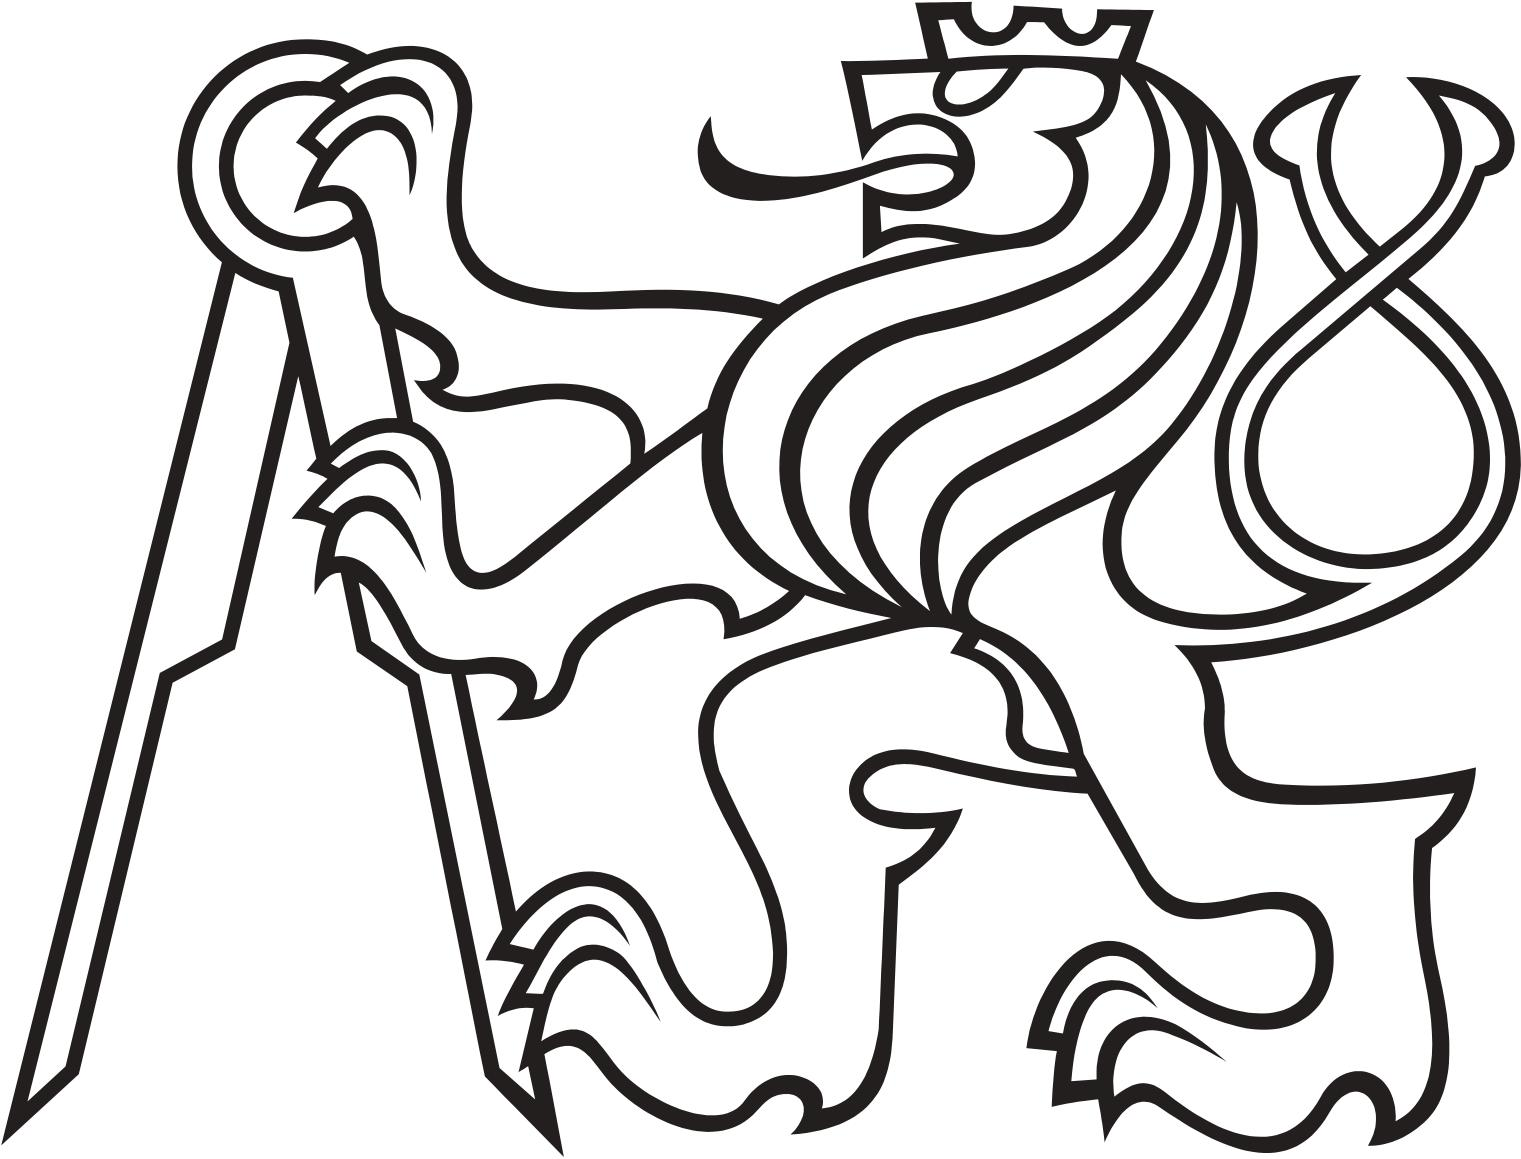
\includegraphics[width=0.3\textwidth]{src/ctu_logo_black.jpg}

%========== Date ==========
\vfill\vfill
{\large\monthyeardate\today}
% Push the date up 1/4 of the remaining page
\vfill
\end{titlepage}

%========== Blank page ==========
\newpage\blankpage

% %========== Assignment ==========
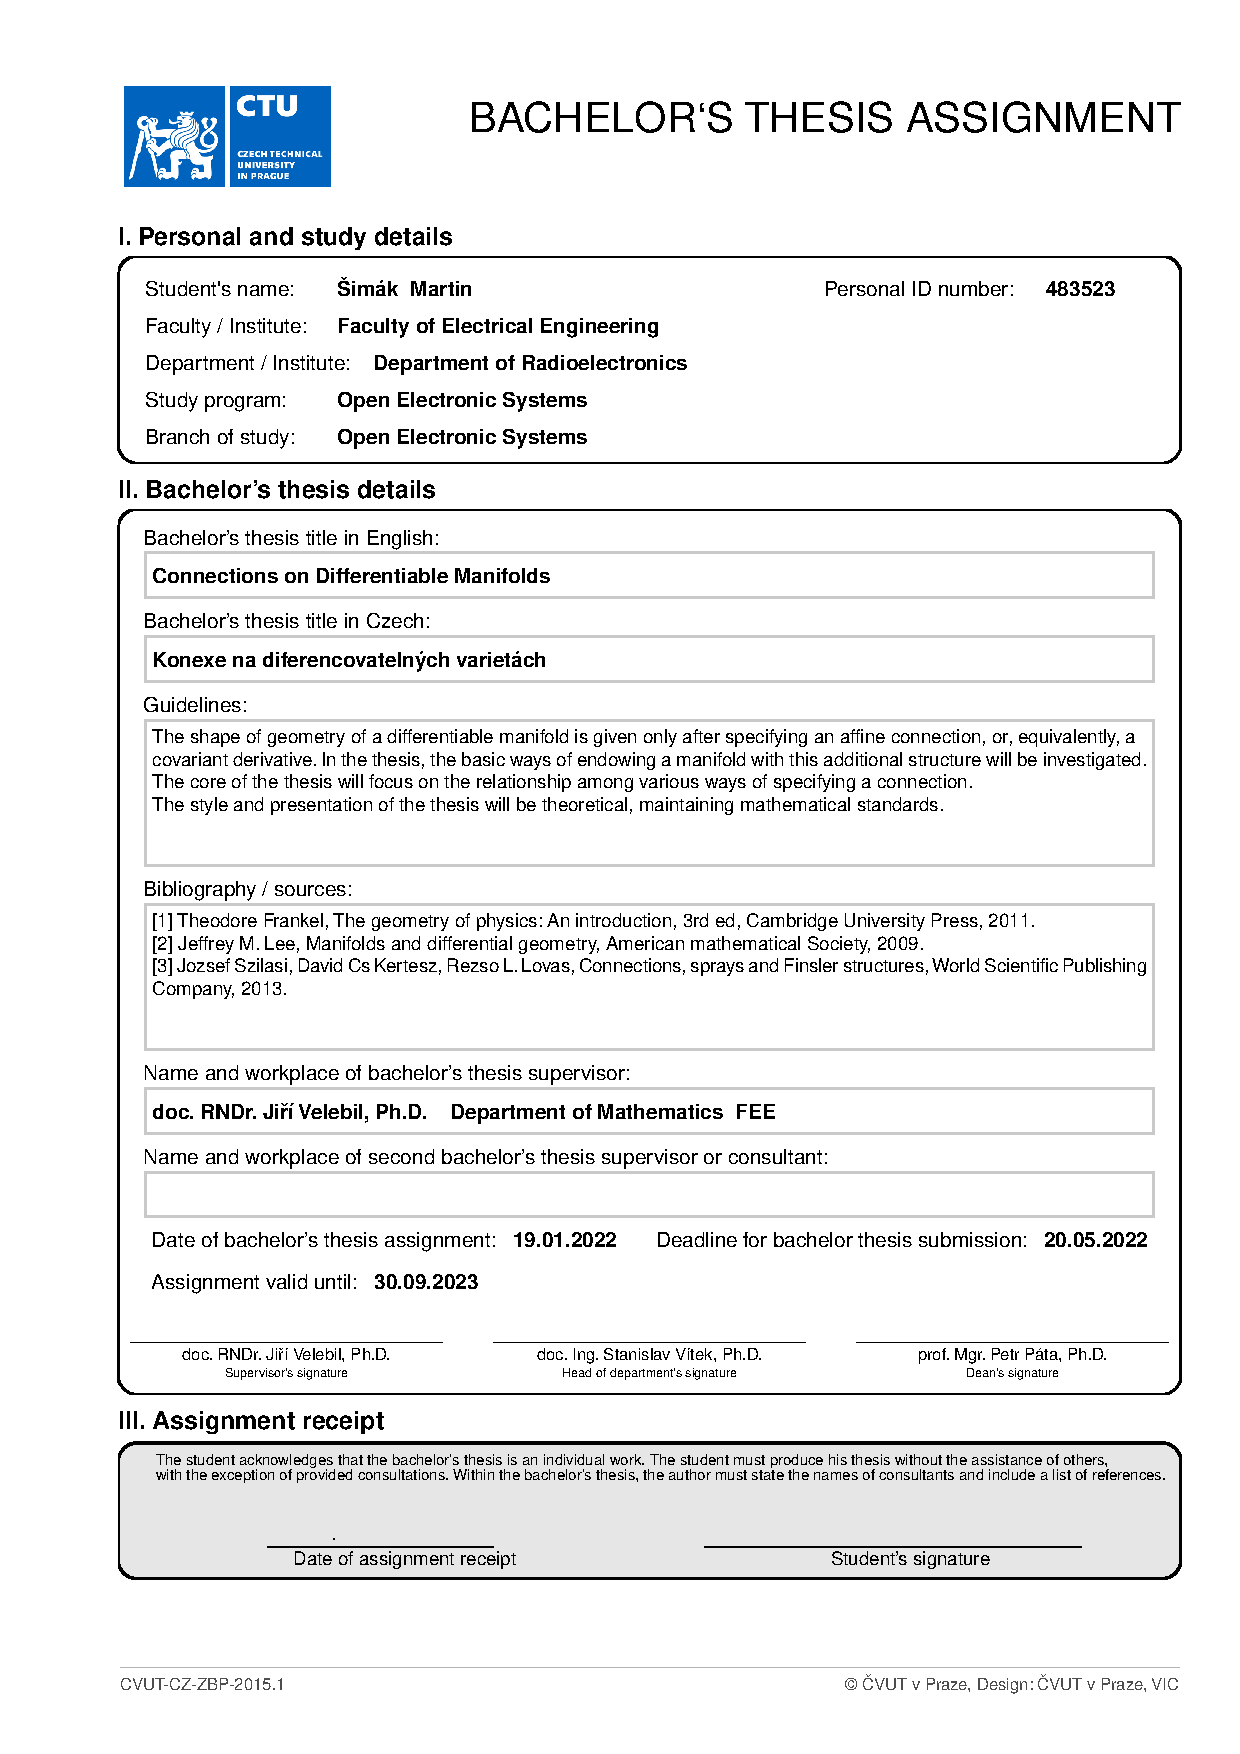
\includepdf[pages=-]{src/assignment.pdf}

% Start counting pages in roman numerals
\pagenumbering{roman}

% %========== Declaration ==========
% \clearpage
\vspace*{\fill}
\noindent\textbf{Declaration}\\[0.25cm]
I declare that I completed the presented thesis independently and that all used sources are quoted in accordance with the Methodological instructions that cover the ethical principles for writing an academic thesis.\\
\hrule\vspace*{1cm}
\begin{otherlanguage}{czech}
    \noindent\textbf{Prohlášení}\\[0.25cm]
    Prohlašuji, že jsem předloženou práci vypracoval samostatně a že jsem uvedl veškeré použité informační zdroje v souladu s Metodickým pokynem o dodržování etických principů při přípravě vysokoškolských závěrečných prací.\\
    \begin{center}
        \begin{minipage}{0.45\textwidth}
            \begin{flushleft}
                V Praze \hdashrule{3cm}{0.5pt}{2pt}
            \end{flushleft}
        \end{minipage}
        ~
        \begin{minipage}{0.45\textwidth}
            \begin{flushright}
                \noindent\begin{tabular}{c}
                    \\
                    \hdashrule{4cm}{0.5pt}{2pt}\\
                    Martin Šimák
                \end{tabular}
            \end{flushright}
        \end{minipage}
    \end{center}
\end{otherlanguage}
\clearpage

% %========== Acknowledgements ==========
% \clearpage
\vspace*{\fill}
\noindent\textbf{Acknowledgements}\\[0.25cm]
Above all, I would like to thank my supervisor, doc. Ing. Pavel Hazdra, Ph.D., for his professional help, willingness, and reliable correspondence throughout our collaboration, which took place remotely during my double degree program in cooperation with the National Taiwan University of Science and Technology. I would also like to thank my supervisor, Ding-Bing Lin, who is responsible for the content of this thesis at the partner university, for his initiative and valuable assistance, especially in the design production. Last but not least, I would like to thank all my loved ones who supported me from afar throughout my studies, especially my family and friends. Special thanks go to Ester \foreignlanguage{czech}{Jančaříková} for standing by me and helping me through difficult times.\\
\hrule\vspace*{1cm}
\begin{otherlanguage}{czech}
    \noindent\textbf{Poděkování}\\[0.25cm]
    Především bych rád poděkoval svému vedoucímu, doc. Ing. Pavlu Hazdrovi, Ph.D., za jeho odbornou pomoc, vstřícnost, a ochotu v podobě spolehlivé korespondence během spolupráce, která probíhala distančně v rámci mého studia double degree programu ve spolupráci s National Taiwan University of Science and Technology. Dále děkuji svému vedoucímu Ding-Bing Linovi, který odpovídá za náplň této práce na partnerské univerzitě, za jeho iniciativu a cennou pomoc, zejména při výrobě návrhu. V neposlední řadě bych rád poděkoval všem svým blízkým, kteří mě na dálku podporovali během celého studia, zejména své rodině a přátelům. Zvláštní poděkování na závěr potom patří Ester Jančaříkové za to, že stála při mě a byla mi oporou v nelehkých chvílích.
\end{otherlanguage}
\clearpage

% %========== Abstract ==========
% \clearpage
\noindent\textit{Title:}\\
\textbf{Dual Circularly Polarized Waveguide Antenna}\\[0.25cm]
\textit{Author:} Martin Šimák\\[0.25cm]
\textit{Study programme:} Electronics and Communications\\[0.25cm]
\textit{Supervisor:} doc. Ing. Pavel Hazdra, Ph.D., Department of Electromagnetic Field FEE\\[0.25cm]
\textit{Abstract:}\\
This thesis details the design, simulation, fabrication, and measurement of a novel dual circularly polarized antenna operating in the $\frequencyrange$ band. The system comprises a square waveguide polarizer with chamfered corners, a dual-coaxial feed, and a conical horn antenna. The polarizer generates right-hand and left-hand circular polarization by selectively exciting one of the two fundamental modes of the square waveguide. The dual coaxial feed provides the necessary excitation. The conical horn, designed using Antenna Magus and adapted to the polarizer, achieves a target gain of $\qty{15}{dBi}$. CST Studio Suite was used for electromagnetic simulations, while Python with SciPy enabled dynamic optimization for enforcing geometric constraints. The fabricated antenna's measured performance closely aligns with simulations, demonstrating an axial ratio below $\qty{5}{dB}$ across the band and a measured gain of approximately $\qty{18}{dBi}$ at the centre frequency. This work contributes to a compact, manufacturable, dual circularly polarized antenna design with potential applications in satellite communications, radar, and other wireless systems.\\[0.25cm]
\textit{Keywords:} circular polarization, waveguide polarizer, dual-feed, conical horn antenna, hexagonal waveguide, eigenmode analysis, electromagnetic simulation\\[0.5cm]
\begin{otherlanguage}{czech}
    \noindent\textit{Název práce:}\\
    \textbf{Duálně kruhově polarizovaná vlnovodová anténa}\\[0.25cm]
    \textit{Autor:} Martin Šimák\\[0.25cm]
    \textit{Studijní program:} Elektronika a komunikace\\[0.25cm]
    \textit{Vedoucí:} doc. Ing. Pavel Hazdra, Ph.D., Katedra elektromagnetického pole FEL\\[0.25cm]
    \textit{Abstrakt:}\\
    Tato diplomová práce popisuje návrh, simulaci, výrobu a měření duální kruhově polarizované antény pracující v pásmu $\frekvencnipasmo$. Systém se skládá ze čtvercového vlnovodného polarizátoru se zkosenými rohy, dvojitého koaxiálního napájení a kuželové antény. Polarizátor generuje pravotočivou a levotočivou kruhovou polarizaci selektivně buzené jedním ze dvou základních módů čtvercového vlnovodu. Potřebné buzení zajišťuje duální koaxiální napájení. Kuželová anténa navržená pomocí programu Antenna Magus a přizpůsobená polarizátoru dosahuje cílového zisku $\qty{15}{dBi}$. Pro elektromagnetické simulace byla použit software CST Studio Suite, zatímco Python s použitím knihovny SciPy umožnil dynamickou optimalizaci pro vynucení geometrických omezení. Naměřený výkon zhotovené antény se přesně shoduje se simulacemi a vykazuje osový poměr pod $\qty{5}{dBi}$ v celém pásmu a naměřený zisk přibližně $\qty{18}{dBi}$ na střední frekvenci. Tato práce přináší kompaktní, vyrobitelnou konstrukci duální kruhově polarizované antény s potenciálním využitím v satelitní komunikaci, radarové technice a dalších bezdrátových systémech.\\[0.25cm]
    \textit{Klíčová slova:} kruhová polarizace, vlnovodný polarizátor, duální napájení, kuželová anténa, hexagonální vlnovod, analýza vlastních módů, elektromagnetická simulace\\[0.5cm]
\end{otherlanguage}
\clearpage

% Start counting pages in arabic numerals
\pagenumbering{arabic}

%========== Table of contents ==========
\tableofcontents

%========== List of figures ==========
\listoffigures

%========== Introduction ==========
\chapter*{Introduction}
\label{chap:introduction}
\addcontentsline{toc}{chapter}{\nameref{chap:introduction}}

\lipsum[1-2]
% Do not write a couple of words on literature survey. Present the difference construction and design choices, compare them both theoretically and by the results presented in gathered papers, but in their respective sections of the design process. Use them a nice foreword for each of the parts, going through existing approaches.

% Say a few words about the simulation software of choice, the CST Studio Suite.

% Maybe chat about frequency band.

% Throughout the theoretical chapter, I omit using the common \emph{del}, or \emph{nabla}, notation for the vector differential operator $\nabla$ which gives rise to the formally proper differential operators of gradient ($\nabla$), divergence ($\nabla\cdot$), curl ($\nabla\times$), and sometimes even the Laplace operator ($\nabla\cdot\nabla$ or $\nabla^2$). Instead, I will use the standard notations of $\Grad$, $\Div$, $\Curl$, and $\Delta$, respectively. While I am aware of the mnemonic merits it brings when working in coordinates, this does not come to fruition as I do not carry out any computations in this text. On the other hand, there are various reasons to avoid it, such as that it promotes a notational ambiguity with the covariant derivative used in differential geometry, or to distinguish the individual operators at first sight better.
% \nomenclature{$\Grad$}{gradient }%
% \nomenclature{$\Div$}{divergence }%
% \nomenclature{$\Curl$}{curl }%
% \nomenclature{$\Delta$}{Laplace operator }%

\paragraph*{Synopsis.} In \textbf{\cref{chap:electrodynamics}}, \lipsum[4]

\paragraph*{Methodology.} \lipsum[4]


%========== Chapter 1: Electrodynamics of guided waves ==========
\chapter{Electrodynamics of guided waves}
\label{chap:electrodynamics}
This chapter establishes the theoretical foundation for the analysis and design of a waveguide-based antenna system. Beginning with Maxwell's equations and general description of electromagnetic fields in various settings relevant to this work, the wave equations governing guided waves are derived, and their solutions are analysed to elucidate the behaviour of electromagnetic fields within waveguides. This analysis provides a framework for understanding the operation of structures designed in the following chapters. While focusing on the essential elements of waveguide theory, this chapter provides a comprehensive treatment of the subject and establishes the notation used throughout this work.

The exposition endeavours to take inspiration and build upon the foundations laid in \parencite{balanis:advanced-engineering-electromagnetics,griffiths:introduction-to-electrodynamics,zangwill:modern-electrodynamics}, incorporating personal insights and notational preferences to present a cohesive theoretical framework for further chapters.

\section{Fundamentals of electrodynamics}
\label{sec:fundamentals-of-electrodynamics}
In this section, the fundamental principles of electromagnetism are presented, starting with Maxwell's equations, which encapsulate the relationships between electric and magnetic fields and their sources. The response of different materials to these fields is then explored through the introduction of \emph{constitutive relations}. Finally, the focus is shifted to the behaviour of electromagnetic fields at material boundaries, providing essential \emph{boundary conditions} for solving electromagnetic problems.

\subsection{Maxwell's equations}
The differential form of Maxwell's equations, as presented below, constitutes the cornerstone of classical electromagnetism, providing a complete%
    \footnote{For actual completeness, save for some special properties stemming from interactions in matter, the equations must also be supplemented by the Lorentz's force law $\vec F = q(\vec E + \vec v \times \vec B)$.}
framework for analysing electromagnetic phenomena at any point in space and time. These equations summarize the relations between \emph{electric field}~$\vec E$ and \emph{magnetic field}~$\vec B$ and their sources due to charge densities~$\rho$, current densities~$\vec J$, or the changing of the fields themselves. To ensure the validity of these expressions, let us assume that the field vectors are well-behaved functions, exhibiting continuity and possessing continuous derivatives. This assumption holds for most electromagnetic systems, with exceptions arising at interfaces between distinct media where abrupt changes in charge and current densities may occur.

\begin{subequations}
    \label[pluralequation]{subeq:maxwell-general}
    \noindent\centering
    \begin{minipage}{0.45\textwidth}
        \begin{align}
            \label{eq:maxwell-general-div-e}
            \div\vec E &= \frac1{\epsilon_0}\rho_{\mathrm e},
        \\
            \label{eq:maxwell-general-curl-e}
            \curl\vec E &= -\mu_0\vec J_{\mathrm m} - \partial_t\vec B,
        \end{align}
    \end{minipage}
    \hfill
    \begin{minipage}{0.45\textwidth}
        \begin{align}
            \label{eq:maxwell-general-div-b}
            \div\vec B &= \mu_0\rho_{\mathrm m},\vphantom{\frac1{\epsilon_0}}
        \\
            \label{eq:maxwell-general-curl-b}
            \curl\vec B &= \mu_0\vec J_{\mathrm e} + \mu_0\epsilon_0\partial_t\vec E,
        \end{align}
    \end{minipage}
    \nomenclature{$\partial_\xi$}{partial derivative w.r.t. variable $\xi$ }%
    \nomenclature{$\vec E$}{electric field }%
    \nomenclature{$\vec B$}{magnetic field }%
    \nomenclature{$\rho_{\mathrm e}$}{electric charge density }%
    \nomenclature{$\rho_{\mathrm m}$}{magnetic charge density }%
    \nomenclature{$\vec J_{\mathrm e}$}{electric current density }%
    \nomenclature{$\vec J_{\mathrm m}$}{magnetic current density }%
    \bigskip
\end{subequations}

There is one oddity about \cref{subeq:maxwell-general} and that is the inclusion of the magnetic charge density $\rho_{\mathrm m}$ and magnetic current density $\vec J_{\mathrm m}$ which are part of the \enquote{generalized concept}. Although these quantities, in spite of diligent search, were never physically observed, their introduction establishes a pleasing balance in Maxwell's equations while being theoretically sound as well. This concept is further utilized when solving advanced physical problems in applied physics and engineering. This is facilitated by the introduction of equivalent magnetic charge and current which can be used to conveniently express fields as if generated by these fictitious sources, especially in problems where the exact form of the electromagnetic field would otherwise be complicated to elucidate.

Mathematically, \cref{subeq:maxwell-general}, like any differential equations, form a complete problem only when supplemented with suitable boundary conditions in a more traditional sense, such as behaviour of the vector fields \enquote{in infinity}. These are typically \enquote{obvious} from the problem-solving context, e.g., fields vanishing at large distance from localized charge distribution, etc.

\subsection{Electromagnetic properties of matter}
Although Maxwell's equations in their fundamental form \eqref{subeq:maxwell-general} provide a complete description of electromagnetic phenomena, an alternative formulation offers a more convenient approach for analysing materials susceptible to electric and magnetic polarization.

Within such media, the total electric charge density~$\rho_{\mathrm e}$ can be expressed as a sum of the \emph{free charge} density~$\rho_{\mathrm f}$, which constitutes the \emph{actual source} charge,%
    \footnote{It is important to reinforce the idea that the magnetic charge and current are fictitious \enquote{source} quantities. Therefore, they are already, by definition, purely \emph{free} quantities.}
and the \emph{bound charge}~$\rho_{\mathrm b}=-\div\vec P$, produced by an electric polarization~$\vec P$ of the material. Moreover, changing electric fields also induce changing polarization, producing \emph{polarization current}~$\vec J_{\mathrm p}=\partial_t\vec P$ which add to the \emph{free current}~$\vec J_{\mathrm f}$. Similarly to electric polarization, a magnetic polarization~$\vec M$ results in a bound current~$\vec J_{\mathrm b}=\curl\vec M$. These effects, inherently connected to the susceptibility of materials to be polarized, hence influence the total electromagnetic field in their vicinity. This led to the introduction of auxiliary field quantities that account for the presence of such media\\
\begin{subequations}
    \label[pluralequation]{subeq:auxiliary-fields}
    \noindent\centering
    \begin{minipage}{0.45\textwidth}
        \begin{align}
            \label{eq:eq:auxiliary-field-d}
            \vec D &= \epsilon_0(\vec E + \vec P)\vphantom{\frac{1}{\mu_0}},
        \end{align}
    \end{minipage}
    \hfill
    \begin{minipage}{0.45\textwidth}
        \begin{align}
            \label{eq:eq:auxiliary-field-h}
            \vec H &= \frac{1}{\mu_0}\vec H - \vec M.
        \end{align}
    \end{minipage}
    \nomenclature{$\vec D$}{auxiliary electric field }%
    \nomenclature{$\vec H$}{auxiliary magnetic field }%
    \bigskip
\end{subequations}\\

This approach allows for expressing Maxwell's equations in a form that directly relates the electric and magnetic fields to the free charge and free current, which are sources that can be controlled directly. Using the field quantities defined by \cref{subeq:auxiliary-fields}, Maxwell's \cref{subeq:maxwell-general} read\\
\begin{subequations}
    \label[pluralequation]{subeq:maxwell-general-matter}
    \noindent\centering
    \begin{minipage}{0.45\textwidth}
        \begin{align}
            \label{eq:maxwell-general-matter-div-d}
            \div\vec D &= \rho_{\mathrm f},
        \\
            \label{eq:maxwell-general-matter-curl-e}
            \curl\vec E &= -\vec J_{\mathrm m} - \partial_t\vec B,
        \end{align}
    \end{minipage}
    \hfill
    \begin{minipage}{0.45\textwidth}
        \begin{align}
            \label{eq:maxwell-general-matter-div-b}
            \div\vec B &= \rho_{\mathrm{m}},
        \\
            \label{eq:maxwell-general-matter-curl-h}
            \curl\vec H &= \vec J_{\mathrm f} + \partial_t\vec D,
        \end{align}
    \end{minipage}
    \bigskip
\end{subequations}

While \cref{subeq:maxwell-general-matter} effectively express electromagnetic laws within media, their hybrid notation, involving both $\vec E$ and $\vec D$, and both $\vec B$ and $\vec H$, necessitates the use of \emph{constitutive relations}. These relations, which establish correspondence between the respective electric and magnetic field quantities, are material-dependent and reflect the specific response of a medium to electric and magnetic fields. In general, these relationships can be expressed as
\begin{subequations}
    \label[pluralequation]{subeq:constitutive-relations}
    \begin{align}
        \label{eq:constitutive-relation-permittivity}
        \vec D &= \hat\epsilon \ast \vec E,
    \\
        \label{eq:constitutive-relation-permeability}
        \vec B &= \hat\mu \ast \vec H,
    \end{align}
    \nomenclature{$\epsilon$}{permittivity }%
    \nomenclature{$\mu$}{permeability }%
    \index{constitutive relations}
    \index{constitutive parameters}
\end{subequations}
where $\hat\epsilon$ and $\hat\mu$ are the material's \emph{permittivity} and \emph{permeability}, respectively, and the asterisk denotes \emph{convolution}.

\begin{remark}
    In formulations of akin to \cref{subeq:maxwell-general-matter}, with emphasis on the separation of free and bound sources, some authors prefer to further dissect the free current, too. This current is generally conceptualized as the current \enquote{not directly tied to the bound charges} within a material. To name a few commonly recognized, \emph{convection current}, \emph{beam current}, or \emph{conduction current}. It is the conduction current which is, in electrical engineering, especially worth mentioning because it arises from the movement of charges, typically electrons, that can move freely throughout the material. This kinetic energy of charges in conductors is the main cause of losses in waveguides and can be expressed by
    \begin{align}
        \label{eq:constitutive-relation-conductivity}
        \vec J_{\mathrm c} &= \hat\sigma \ast \vec E,
        \nomenclature{$\sigma$}{conductivity }%
    \end{align}
    where $\hat\sigma$ is the material's \emph{conductivity}. \Cref{eq:constitutive-relation-conductivity}, together with \cref{subeq:constitutive-relations}, completes the required set of constitutive relations.
\end{remark}

The \emph{constitutive parameters} $\hat\epsilon$, $\hat\mu$, and $\hat\sigma$, generally represented as complex second-rank tensors, establish the relationship between the applied electromagnetic fields and the material's response. The functional dependencies of these tensors provide a classification scheme for material properties:
\begin{itemize}
    \item \emph{Linearity:} A material is classified as linear if its constitutive parameters are independent of the applied field strength; otherwise, it is considered nonlinear.
    \item \emph{Homogeneity:} If the constitutive parameters are invariant with respect to position within the material, it is deemed homogeneous; conversely, spatial dependence indicates an inhomogeneous medium.
    \item \emph{Isotropy:} Materials exhibiting constitutive parameters independent of the applied field's direction are classified as isotropic. Conversely, direction-dependent parameters signify an anisotropic material, with crystals being a prime example.
    \item \emph{Dispersion:} Materials whose constitutive parameters exhibit frequency dependence are categorized as dispersive. While some materials demonstrate negligible frequency dependence and can be effectively considered nondispersive, all materials encountered in practice exhibit some degree of dispersion.
\end{itemize}

\begin{example}[Constitutive relations in free space]
    In the simplest case of free space, equations~\eqref{eq:constitutive-relation-permittivity},~\eqref{eq:constitutive-relation-permeability},~and~\eqref{eq:constitutive-relation-conductivity} become
    \begin{subequations}
        \begin{align}
            \hat\epsilon &= \epsilon_0 \approx 8.854\times 10^{-12}\ \unit{F.m^{-1}},
        \\
            \hat\mu &= \mu_0 = 4\pi\times 10^{-7}\ \unit{H.m^{-1}},
        \\
            \hat\sigma &= \sigma_0 = 0\ \unit{S.m^{-1}}.
        \end{align}
    \end{subequations}
\end{example}

\subsection{Boundary conditions}
While the differential form of Maxwell's equations is a powerful tool for analysing electromagnetic fields within continuous media, material boundaries introduce discontinuities that require special treatment. These discontinuities in the fields arise at interfaces between media with different electrical properties or at surfaces carrying charge or current densities. To accurately describe the behaviour of the fields across such boundaries, Maxwell's equations in their integral form, which naturally incorporate these discontinuities, are more convenient. This form is obtained by applying integral theorems from vector calculus to \cref{subeq:maxwell-general-matter} which then take on the form of
\begin{subequations}
    \label[pluralequation]{subeq:maxwell-equations-integral}
    \begin{align}
        \label{eq:maxwell-equations-integral-div-d}
        \oint_S \vec D \cdot \d\vec a &= Q_{\mathrm{e}},
    \\
        \label{eq:maxwell-equations-integral-curl-e}
        \oint_{\partial S} \vec E \cdot \d\vec l &= -\int_S \vec J_{\mathrm m} \cdot \d\vec a - \frac{\d}{\d t}\int_S \vec B \cdot \d\vec a,
    \\
        \label{eq:maxwell-equations-integral-div-b}
        \oint_S \vec B \cdot \d\vec a &= Q_{\mathrm{m}},
    \\
        \label{eq:maxwell-equations-integral-curl-h}
        \oint_{\partial S} \vec H \cdot \d\vec l &= \int_S \vec J_{\mathrm e} \cdot \d\vec a + \frac{\d}{\d t}\int_S \vec D \cdot \d\vec a,
    \end{align}
    \nomenclature{$\partial\Omega$}{boundary of set $\Omega$ }%
\end{subequations}
\index{boundary conditions}
where $S$ is any closed surface.

Consider a boundary between two different media. The first medium is characterized by permittivity $\epsilon_1$ and permeability $\mu_1$, while the second medium is characterized by permittivity $\epsilon_2$ and permeability $\mu_2$. At this interface, electric and magnetic surface charge densities, denoted by $q_{\mathrm f}$ and $q_{\mathrm m}$, respectively, may be present. Additionally, electric and magnetic surface current densities, denoted by $j_{\mathrm f}$ and $j_{\mathrm m}$, respectively, may also exist. The general \emph{boundary conditions} for electrodynamics are then obtained by applying \cref{subeq:maxwell-equations-integral} to arbitrary surfaces encompassing a portion of the interface, yielding\\
\begin{subequations}
    \label[pluralequation]{subeq:boundary-conditions}
    \noindent\centering
    \begin{minipage}{0.45\textwidth}
        \begin{align}
            \label{eq:boundary-conditions-d-normal}
            \vec e_n \cdot (\vec D_1 - \vec D_2) &= q_{\mathrm f},
        \\
            \label{eq:boundary-conditions-e-tangential}
            -\vec e_n \times (\vec E_1 - \vec E_2) &= \vec j_{\mathrm m},
        \end{align}
    \end{minipage}
    \hfill
    \begin{minipage}{0.45\textwidth}
        \begin{align}
            \label{eq:boundary-conditions-b-normal}
            \vec e_n \cdot (\vec B_1 - \vec B_2) &= q_{\mathrm m},
        \\
            \label{eq:boundary-conditions-H-tangential}
            \vec e_n \times (\vec H_1 - \vec H_2) &= \vec j_{\mathrm f}.
        \end{align}
    \end{minipage}
    \bigskip
\end{subequations}

\section{Electromagnetic waves}
\label{sec:electromagnetic-waves}
Having established the foundations of electromagnetism, the focus is now shifted to one of its most significant consequences: the existence of electromagnetic waves. In this section, the manner in which Maxwell's equations predict the propagation of these waves is explored.  The wave equations for the electric and magnetic fields are derived, revealing their interconnected nature and their ability to sustain each other even in the absence of sources. Subsequently, the simplest and most fundamental solutions to these equations, \emph{monochromatic plane waves}, are investigated. Finally, the confinement and guidance of these plane waves within conducting cavities is examined, laying the groundwork for understanding waveguides and resonant structures.

\subsection{The wave equations}
\label{subsection:the-wave-equations}
Maxwell's equations provide a comprehensive description of electromagnetic phenomena, but their coupled nature can make them challenging to solve directly. To facilitate analysis, particularly in source-free regions, it's often advantageous to decouple the equations and express them in terms of the electric and magnetic fields individually. Inside regions with no \emph{free} charge or \emph{free} current, Maxwell's \cref{subeq:maxwell-general-matter} take on the form of\\
\begin{subequations}
    \label[pluralequation]{subeq:maxwell-sourceless}
    \noindent\centering
    \begin{minipage}{0.45\textwidth}
        \begin{align}
            \label{eq:maxwell-sourceless-div-d}
            \div \vec D &= 0,
        \\
            \label{eq:maxwell-sourceless-curl-e}
            \curl \vec E &= -\partial_t\vec B,
        \end{align}
    \end{minipage}
    \hfill
    \begin{minipage}{0.45\textwidth}
        \begin{align}
            \label{eq:maxwell-sourceless-div-b}
            \div\vec B &= 0,
        \\
            \label{eq:maxwell-sourceless-curl-h}
            \curl\vec H &= \sigma\vec E + \partial_t\vec D.
        \end{align}
    \end{minipage}\bigskip
\end{subequations}\\
Furthermore, if the medium is \emph{linear} and \emph{homogeneous}, \cref{eq:maxwell-sourceless-curl-h} can be fully expressed in terms of $\vec E$. With this simplification, applying the curl to \cref{eq:maxwell-sourceless-curl-e,eq:maxwell-sourceless-curl-h} yields\\
\begin{subequations}
    \label[pluralequation]{subeq:wave-equations-lossy}
    \noindent\centering
    \begin{minipage}{0.45\textwidth}
        \begin{align}
            \label{eq:wave-equation-e}
            \Delta\vec E &= \mu\sigma\partial_t\vec E + \mu\epsilon\partial^2_t\vec E,
        \end{align}
    \end{minipage}
    \hfill
    \begin{minipage}{0.45\textwidth}
        \begin{align}
            \label{eq:wave-equation-b}
            \Delta\vec B &= \mu\sigma\partial_t\vec B + \mu\epsilon\partial^2_t\vec B.
        \end{align}
    \end{minipage}\bigskip
\end{subequations}

Therefore, electric and magnetic fields in linear homogeneous media both clearly satisfy the wave equation with a linear damping term $\mu\sigma\partial_t$, introduced by conductive losses. Moreover, in regions with $\sigma = 0$, such as free space or ideal insulators, \cref{subeq:wave-equations-lossy} simplify even more to\\
\begin{subequations}
    \label[pluralequation]{subeq:wave-equations-lossless}
    \noindent\centering
    \begin{minipage}{0.45\textwidth}
        \begin{align}
            \label{eq:wave-equation-e-lossless}
            \Delta\vec E &= \mu\epsilon\partial^2_t\vec E,
        \end{align}
    \end{minipage}
    \hfill
    \begin{minipage}{0.45\textwidth}
        \begin{align}
            \label{eq:wave-equations-b-lossless}
            \Delta\vec B &= \mu\epsilon\partial^2_t\vec B,
        \end{align}
    \end{minipage}\bigskip
\end{subequations}\\
taking on the form of classical wave equations which are ubiquitous in physics. This also immediately gives rise to the formula
\begin{align}
    v &= \frac{1}{\sqrt{\epsilon\mu}} = \frac{c}{\sqrt{\epsilon_r\mu_r}}
\end{align}
for the speed of electromagnetic waves in linear homogeneous media.

\begin{remark}
    \label{remark:nonequivalence-of-wave-equations-with-maxwells-equations}
    Compared with the original Maxwell's \cref{subeq:maxwell-general-matter}, these equations form two systems of second-order partial differential equations but are now decoupled and provide us with an additional solving method for given boundary-value problems. However, it is important to note that the wave \cref{eq:wave-equation-e,eq:wave-equation-b} were derived from Maxwell's \cref{subeq:maxwell-sourceless} by differentiation. This impedes their mathematical equivalence. More specifically, as stated in~\parencite{griffiths:introduction-to-electrodynamics}, whereas every solution to Maxwell's equations is also a solution for the wave equations, the converse is not true.
\end{remark}

\subsection{Monochromatic plane waves}
\index{monochromatic plane wave}
The electromagnetic theory presented thus far describes general vector fields that vary in space and time. However, as shown in \cref{subsection:the-wave-equations}, electromagnetic fields in source-free regions exhibit wave behaviour. Nonetheless, these time-varying vector fields remain complex and challenging to analyse in practical systems. Consider the elementary solution to the wave equation
\begin{align}
    \label{eq:monochromatic-plane-wave}
    \hat{\vec\psi}(\vec r,t) &= \hat{\vec\Psi}_0\exp\[\i\(\hat{\vec k} \cdot \vec r-\omega t\)\].
\end{align}
\nomenclature{$\vec k$}{wave vector }%
Here, $\hat{\vec k}$ is the complex \emph{wave vector} indicating the direction of wave propagation, and $\omega$ is the angular frequency of the wave. \Cref{eq:monochromatic-plane-wave} is expressed in terms of a \emph{complex wave function} with a \emph{complex amplitude} $\hat{\vec\Psi}_0 \equiv \vec\Psi_0\e^{\i\delta}$. This quantity encapsulates both the \emph{real amplitude} $\vec\Phi_0$ and the \emph{phase shift} $\delta$, of the physical wave. A sinusoidal wave representing this solution in physical reality can be extracted from \cref{eq:monochromatic-plane-wave} using the \emph{Euler's formula}, yielding
\begin{align}
    \label{eq:sinusoidal-wave}
    \vec{\psi}(\vec r, t) &= \Re\[\hat{\vec\Psi}_0\exp\[\i\(\hat{\vec k} \cdot \vec r-\omega t+\delta\)\]\] = \Re\[\hat{\vec\psi}(\vec r, t)\].
\end{align}

\begin{remark}
    Clearly, if \cref{eq:sinusoidal-wave} satisfies \cref{subeq:wave-equations-lossless} and Maxwell's equations, the same holds true for \cref{eq:monochromatic-plane-wave}, as the imaginary part differs from the real part only by the replacement of sine with cosine.
\end{remark}

\Cref{eq:monochromatic-plane-wave} serves as as an established elementary solution to the general wave equation, and hence also to \cref{subeq:wave-equations-lossless}. Substituting this solution into \cref{subeq:wave-equations-lossy}, it becomes evident that these \enquote{lossy wave equations} also admit plane-wave solutions. Furthermore, this substitution allows for the derivation of a general formula for the complex \emph{wavenumber}
\begin{align}
    \label{eq:wave-number}
    \hat k^2 = \hat{\vec k} \cdot \hat{\vec k} = \mu\epsilon\omega^2 + \i\mu\sigma\omega.
\end{align}
In the context of \cref{eq:monochromatic-plane-wave}, it is evident that the real part of the complex wavenumber $\hat k$ is the \emph{actual} wavenumber as it determines the change of phase with spatial propagation. For this reason, the real part is simply denoted $k$ and is called the \emph{phase constant}. In contrast, the imaginary part of $\hat k$ is responsible for the exponential damping, or attenuation, in conductive media, and hence is called the \emph{attenuation constant}.

Waves described by \cref{eq:monochromatic-plane-wave} are called \emph{monochromatic}, or \emph{time-harmonic}, \emph{plane}
waves. Monochromaticity refers to the fact that the wave oscillates at a single frequency $\omega$ through time, while planarity indicates that the fields are uniform over every plane perpendicular to the direction of propagation. Although less common, plane waves could alternatively be called \emph{space-harmonic},%
    \footnote{Therefore, monochromatic plane waves are something one could call \emph{spacetime-harmonic} or simply \emph{harmonic}.}
as both of these terms signify a sinusoidal dependence on a given variable. In the case of monochromaticity, the variable is time, oscillating with an angular frequency $\omega$. Similarly, planarity reflects the waveform repetition in the spatial coordinates, projected into the propagation direction, with a well-defined spatial frequency $k$.

The significance of this particular solution stems from the fact that, in practice, any wave we will be dealing with can be expressed as a linear combination of these monochromatic plane waves, i.e.,
\begin{align}
    \label{eq:fourier-transform}
    \hat{\vec\psi}(\vec r,t) &= \int_{\R^3} \hat{\vec{\Psi}}_0(\vec k)\exp\[\i\(\hat{\vec k} \cdot \vec r-\omega t\)\]\,\d\vec k.
\end{align}
This superposition principle mathematically reflects the Fourier transform over every plane wave corresponding to a given frequency $\omega$. With this formally sound mathematical description, the existence of a unique linear combination for \enquote{any wave we will be dealing with}, as vaguely stated above, can be rigorously established.

Indeed, since any physically realizable signal is square-integrable and has compact support,%
    \footnote{In the field of signal processing, these signal properties are often described as having \emph{finite energy} and \emph{duration}, respectively.}
the existence of its Fourier transform is guaranteed. This implication is granted by recalling that the combination of square-integrability and compact support implies, by the Cauchy-Schwarz inequality, absolute integrability which forms a sufficient condition for the existence of the Fourier transform. Therefore, any such physical signal can be confidently decomposed into a superposition of monochromatic plane waves, as expressed in equation \cref{eq:fourier-transform}. This decomposition into a unique linear combination of plane waves of different frequencies underpins much of the mathematical theory concerning Fourier analysis. For a deeper dive into the mathematical foundations of Fourier integrals, \parencite{titchmarsh:introduction-to-the-theory-of-fourier-integrals} can be consulted. Furthermore, a formulation of Dirichlet conditions which are more attuned to signal processing applications can be found in \parencite{oppenheim:signals-and-systems}.

Because the focus of this text is confined to signals that are physically realizable and thus possess these crucial properties, a restriction of our attention to monochromatic plane waves is justified. Therefore, fields taking on the form of
\begin{subequations}
    \label[pluralequation]{subeq:monochromatic-plane-wave-fields}
    \begin{align}
        \label{eq:monochromatic-plane-wave-e}
        \hat{\vec E}(\vec r, t) &= \hat{\vec E}_0 \exp\[\i\(\hat{\vec k} \cdot \vec r-\omega t\)\],
    \\
        \label{eq:monochromatic-plane-wave-b}
        \hat{\vec B}(\vec r, t) &= \hat{\vec B}_0 \exp\[\i\(\hat{\vec k} \cdot \vec r-\omega t\)\]
    \end{align}
\end{subequations}
are considered, where $\hat{\vec E}_0$ and $\hat{\vec B}_0$ are complex amplitudes.

As discussed in \cref{remark:nonequivalence-of-wave-equations-with-maxwells-equations}, satisfying the wave equations does not guarantee solutions to Maxwell's equations. Substituting the solutions of the wave equations into Maxwell's equations is necessary, as it might refine the solutions or yield more information. As an example, consider the plane waves in vacuum.

\begin{example}[Monochromatic plane waves in free space]
    Substituting \cref{eq:monochromatic-plane-wave-e,eq:monochromatic-plane-wave-b} for the electric and magnetic field in the free-space version of \cref{eq:maxwell-sourceless-div-d,eq:maxwell-sourceless-div-b} read
    \begin{align}
        \vec k \cdot \hat{\vec E}_0 = \vec k \cdot \hat{\vec B}_0 = 0,
    \end{align}
    \nomenclature{$\vec e_\xi$}{unit vector in the $\xi$-direction }%
    i.e., the electromagnetic fields are \emph{transverse}. Furthermore, either of \cref{eq:maxwell-sourceless-curl-e,eq:maxwell-sourceless-curl-h} yields
    \begin{align}
        \hat{\vec B}_0 &= \frac1\omega\(\vec k \times \hat{\vec E}_0\) = \frac 1c\(\vec e_k \times \hat{\vec E}_0\).
    \end{align}
    Clearly, in free space, $\vec E$ and $\vec B$ are \emph{mutually perpendicular} and \emph{in phase}, meaning their oscillations reach their peaks and troughs simultaneously.
    
    To further characterize the plane wave, a \emph{polarization vector} is introduced. This unit vector points in the direction of electric field oscillations, i.e.,
    \begin{align}
        \vec e_n \cdot \vec E &= \vec E
    &
        \norm{\vec e_n} &= 1.
    \end{align}
    \nomenclature{$\vec e_n$}{polarization vector }%
    \index{polarization vector}%
    With this definition, the complete solution to Maxwell's equations for a plane wave in free space takes the form of
    \begin{align}
        \vec E(\vec r, t) &= E_0\cos(\vec k \cdot \vec r - \omega t + \delta) \vec e_n,
    \\
        \vec B(\vec r, t) &= \frac 1c E_0\cos(\vec k \cdot \vec r - \omega t + \delta) (\vec k \times \vec e_n).
    \end{align}

    It's important to note that this transversality of the electromagnetic fields is a specific property of plane waves in free space or lossless media. When waves are confined in waveguides or propagate through lossy media, the fields generally have longitudinal components as well. This distinction arises because the boundary conditions imposed by the waveguide or the interactions with the medium can alter the field structure.
\end{example}

\subsection{Polarization}
\label{subsection:polarization}
A brief examination of the general polarization properties of monochromatic plane waves is now undertaken. For the sake of simplicity, consideration is restricted to propagation within a vacuum. Consequently, the Cartesian coordinate system is aligned such that the unit vector $e_z$ coincides with the unit vector $e_{\vec k}$ which defines the direction of propagation. The remaining real unit vectors, $\vec e_x$ and $\vec e_y$, are then defined such that $(\vec e_x, \vec e_y, \vec e_z)$ constitutes a right-handed orthogonal triad of unit vectors. Thus, the ordered set of vectors $(\vec e_x, \vec e_y)$ forms a basis for the complex amplitude of the electric field E, and the electric field can thereby be expressed as
\begin{align}
    \label{eq:polarization-e}
    \hat{\vec E}(\vec r,t) &= \[\hat E_x\vec e_x + \hat E_y\vec e_y\]\exp\[\i\phi(\vec r,t)\],
\end{align}
where
\begin{align}
    \hat E_x &= E_x\exp\(\i\delta_x\),
&
    \hat E_y &= E_y\exp\(\i\delta_y\),
\end{align}
for some real numbers $E_x$, $E_y$, $\delta_x$, and $\delta_y$, and
\begin{align}
    \phi(\vec r,t) &= \hat{\vec k} \cdot \vec r - \omega t.
\end{align}
Expressing the real part of \cref{eq:polarization-e} yields
\begin{align}
    \label{eq:polarization-e-real-part}
    \Re\[\hat{\vec E}\] &= E_x\cos\(\phi + \delta_x\)\vec e_x + E_y\cos\(\phi + \delta_y\)\vec e_y = A_x\vec e_x + A_y\vec e_y.
\end{align}
Equating the components from the second relation in \cref{eq:polarization-e-real-part} and applying goniometric identities, the following relationships are obtained:
\begin{subequations}
    \begin{align}
        \label{eq:polarization-ellipse-a}
        \frac{A_x}{E_x}\sin(\delta_y)-\frac{A_y}{E_y}\sin(\delta_x) &= \sin(\delta_y-\delta_x)\cos(\phi),
    \\
        \label{eq:polarization-ellipse-b}
        \frac{A_x}{E_x}\sin(\delta_y)-\frac{A_y}{E_y}\sin(\delta_x) &= \sin(\delta_y-\delta_x)\cos(\phi).
    \end{align}
\end{subequations}
Subsequent squaring and addition of \cref{eq:polarization-ellipse-a,eq:polarization-ellipse-b} yields
\begin{align}
    \label{eq:polarization-ellipse}
    \(\frac{A_x}{E_x}\)^2 + \(\frac{A_y}{E_y}\)^2 - 2\frac{A_x}{E_x}\frac{A_y}{E_y}\cos\(\delta\) &= \sin^2\(\delta\),
\end{align}
\index{elliptical polarization}
where $\delta \equiv \delta_y-\delta_x$. Clearly, \cref{eq:polarization-ellipse} defines an ellipse in the plane transverse to the propagation direction. Accordingly, it can be stated that the general monochromatic plane wave described in \cref{eq:monochromatic-plane-wave} exhibits \emph{elliptical polarization}. The eccentricity and orientation of the ellipse are related to the phase difference $\delta$ and the amplitude ratio $E_y/E_x$. Inspecting \cref{eq:polarization-ellipse}, two special types of polarization can be identified for specific parameter values.

\paragraph{Linear polarization.\index{linear polarization}} The first situation arises when the polarization ellipse degenerates into a straight line. This condition occurs when the electric field components are either in-phase or out-of-phase by half-wavelength, i.e.,
\begin{align}
    \label{eq:polarization-linear-condition}
    \delta = \delta_y-\delta_x = m\pi, \quad m \in \N_0.
\end{align}
This situation corresponds to \emph{linear polarization} and \cref{eq:polarization-e-real-part} is rendered as
\begin{align}
    \label{eq:polarization-linear-e}
    \Re\[\hat{\vec E}(\vec r,t)\] &= \[E_x\vec e_x \pm E_y\vec e_y\]\cos\(\phi + \delta_x\).
\end{align}

\paragraph{Circular polarization.\index{circular polarization}} The alternative scenario arises when the polarization ellipse simplifies into a circle. This simplification occurs exclusively when the orthogonal electric field components possess equal amplitude and are out-of-phase by one-quarter wavelength, i.e.,
\begin{align}
    \label{eq:polarization-circular-condition}
    E_x = E_y &= \frac{E}{\sqrt 2},
&
    \delta = \delta_y-\delta_x &= (2m+1)\frac{\pi}{2}, \quad m \in \Z.
\end{align}
This condition corresponds to \emph{circular polarization}, as the tip of the polarization vector traces a circle within every fixed transverse plane. To ascertain the direction of circular movement, the plane $z=0$ is considered. By setting $\delta_x = 0$,%
    \footnote{The choice $\delta_x=0$ is inconsequential to the resulting polarization as it depends only on the phase difference $\delta$.}
\cref{eq:polarization-e-real-part} is expressed as
\begin{align}
    \label{eq:polarization-circular-e-r0}
    \Re\[\hat{\vec E}_\pm(\vec 0,t)\] &= \frac{E}{\sqrt 2}\[\cos(\omega t)\vec e_x \pm \sin(\omega t)\vec e_y\].
\end{align}
This expression demonstrates that, when viewed from the direction defined by $\hat{\vec k}$, the electric field $\hat{\vec E}^+$ represents a circularly polarized wave with the polarization vector rotating anticlockwise, thus defining \emph{left-hand circular polarization} (LHCP). Conversely, the case of $\hat{\vec E}^-$ represents a circularly polarized wave with the polarization vector rotating clockwise, defining \emph{right-hand circular polarization} (RHCP).

The exposition given so far is aligned with Augustin-Jean Fresnel's general definition of elliptical polarization, as presented in his memoir to the French Academy of Sciences on 9 December 1822, wherein the concepts of the three types of polarization--general elliptical polarization, and its specific forms, linear and circular polarization--were coined. The following remark, however, provides an alternative, and often advantageous, approach.

\begin{remark}[Complex basis for circular polarization]
    For the electric field decomposition basis, the following complex conjugate vectors, rather than the Cartesian vectors $\vec e_x$ and $\vec e_y$, are now considered:
    \begin{align}
        \label{eq:polarization-circular-complex-vectors}
        \vec e_+ &= \frac{1}{\sqrt 2}\(\vec e_x + \i\vec e_y\),
    &
        \vec e_- &= \frac{1}{\sqrt 2}\(\vec e_x - \i\vec e_y\).
    \end{align}
    These vectors maintain orthonormality. Using this basis, it is evident that the real part of the thus formed complex electric field
    \begin{align}
        \hat{\vec E}_\pm(\vec r,t) &= E\vec e_\pm\exp\[\i\(\hat{\vec k}\cdot\vec r - \omega t\)\] = \frac{E}{\sqrt 2}\[\vec e_x \pm \i\vec e_y\]\exp\[\i\(\hat{\vec k}\cdot\vec r - \omega t\)\],
    \end{align}
    evaluated at $\vec r = 0$, is equivalent to \cref{eq:polarization-circular-e-r0}. Because the ordered set of vectors defined by \cref{eq:polarization-circular-complex-vectors} constitutes a valid basis for the transverse plane, analogous to the $(\vec e_x,\vec e_y)$ basis, the expression
    \begin{align}
        \hat{\vec E} &= \[E_+\vec e_+ + E_-\vec e_-\]\exp\[\i\phi\]
    \end{align}
    is an equivalent representation to \cref{eq:polarization-e}. Consequently, any monochromatic plane wave can be decomposed into RHCP and LHCP components, in a manner analogous to its decomposition into orthogonal linearly polarized components.
\end{remark}

\subsection{Guided waves}
The behaviour of electromagnetic waves within a waveguide is now explored. To provide a clear framework for analysis, it is assumed that the waveguide walls are perfect electric conductors (PEC), implying the absence of surface sources. This idealization leads to specific boundary conditions\\
\begin{subequations}
    \label[pluralequation]{subeq:guided-waves-boundary-conditions}
    \noindent\centering
    \begin{minipage}{0.45\textwidth}
        \begin{align}
            \label{eq:guided-waves-boundary-condition-e}
            \vec e_n \times \vec E &= 0,
        \end{align}
    \end{minipage}
    \hfill
    \begin{minipage}{0.45\textwidth}
        \begin{align}
            \label{eq:guided-waves-boundary-condition-b}
            \vec e_n \cdot \vec B &= 0.
        \end{align}
    \end{minipage}\bigskip
\end{subequations}\\
It is important to recognize that free charges and currents will be induced on the surface precisely to enforce these constraints.

Furthermore, the focus is placed on monochromatic plane waves propagating along the waveguide. This implies that the electric and magnetic fields have a harmonic time dependence with a single angular frequency $\omega$. The $\hat{\phantom{x}}$ notation is dispensed with as $\hat k$ is real for the cases of interest. The general form of the fields is then given by \cref{subeq:monochromatic-plane-wave-fields} where the $z$-axis is aligned with the waveguide's longitudinal direction. The complex amplitudes of the fields,\\
\begin{subequations}
    \label[pluralequation]{subeq:complex-amplitudes}
    \noindent\centering
    \begin{minipage}{0.45\textwidth}
        \begin{align}
            \label[pluralequation]{subeq:complex-amplitude-e}
            \hat{\vec E}_0 &= E_x\vec e_x + E_y\vec e_y + E_z\vec e_z,
        \end{align}
    \end{minipage}
    \hfill
    \begin{minipage}{0.45\textwidth}
        \begin{align}
            \label[pluralequation]{subeq:complex-amplitude-b}
            \hat{\vec B}_0 &= B_x\vec e_x + B_y\vec e_y + B_z\vec e_z,
        \end{align}
    \end{minipage}\bigskip
\end{subequations}\\
are functions of the transverse coordinates, $x$ and $y$, reflecting the spatial variations of the fields within the waveguide cross-section.

To further simplify the analysis, the waveguide is considered to be source-free, meaning that there are no free charges or currents \emph{impressed} within the waveguide itself. This allows the utilization of the simplified form of Maxwell's equations \eqref{subeq:maxwell-sourceless}. Due to the assumed linearity of the medium within the waveguide, these equations are expressed in terms of $E$ and $B$.

With these assumptions in place, the wave behaviour within the waveguide can be analysed. From \cref{eq:maxwell-sourceless-curl-e,eq:maxwell-sourceless-curl-h}, adapted for a linear medium, a set of coupled differential equations relating the transverse components of the electric and magnetic fields is obtained. These equations can be solved to express the transverse field components in terms of the longitudinal components, taking the form of\\
\begin{subequations}
    \label[pluralequation]{subeq:guided-wave-transverse-fields}
    \noindent\centering
    \begin{minipage}{0.45\textwidth}
        \begin{align}
            \label{eq:guided-wave-ex}
            E_x &= \zeta\(k\partial_xE_z+\omega\partial_yB_z\)\vphantom{\frac{\omega}{c^2}},
        \\
            \label{eq:guided-wave-ey}
            E_y &= \zeta\(k\partial_yE_z-\omega\partial_xB_z\)\vphantom{\frac{\omega}{c^2}},
        \end{align}
    \end{minipage}
    \hfill
    \begin{minipage}{0.45\textwidth}
        \begin{align}
            \label{eq:guided-wave-bx}
            B_x &= \zeta\(k\partial_xB_z-\frac{\omega}{c^2}\partial_yE_z\),
        \\
            \label{eq:guided-wave-by}
            B_y &= \zeta\(k\partial_yB_z+\frac{\omega}{c^2}\partial_xE_z\),
        \end{align}
    \end{minipage}\bigskip
\end{subequations}\\
where $\zeta = \i/((\omega/c)^2-k^2)$. Finally, substituting \cref{subeq:guided-wave-transverse-fields} into \cref{eq:maxwell-sourceless-div-d,eq:maxwell-sourceless-div-b} leads to uncoupled equations
\begin{subequations}
    \label[pluralequation]{subeq:guided-wave-longitudinal-fields}
    \begin{align}
        \label{eq:guided-wave-ez}
        \[\partial^2_x+\partial^2_y+\(\frac{\omega}{c}\)^2-k^2\]E_z &= 0,
    \\
        \label{eq:guided-wave-bz}
        \[\partial^2_x+\partial^2_y+\(\frac{\omega}{c}\)^2-k^2\]B_z &= 0.
    \end{align}
\end{subequations}
\index{Helmholtz equations}
These equations, often referred to as the \emph{Helmholtz equations}, govern the longitudinal field components and play a crucial role in determining the allowed modes of propagation within the waveguide. These modes are categorized based on the presence or absence of longitudinal components in the electric and magnetic fields. \emph{Transverse electric} (TE) waves have $E_z=0$, while \emph{transverse magnetic} (TM) waves have $B_z=0$. The simplest waves, with both $E_z=B_z=0$ are called \emph{transverse electromagnetic} (TEM) waves, but these cannot exist within a hollow waveguide due to boundary conditions.

\begin{remark}[Non-existence of TEM waves in hollow waveguides]
    \label{remark:nonexistence-of-tem-waves-in-hollow-waveguides}
    To further illustrate this point, consider the case of a waveguide with perfectly conducting walls.
    
    Beginning with the scenario where the longitudinal component of the electric field, $E_z$, is zero, it follows from \cref{eq:maxwell-sourceless-div-d} that the divergence of the electric field in the transverse plane must also be zero. Similarly, when the longitudinal component of the magnetic field, $B_z$, is zero, \cref{eq:maxwell-sourceless-curl-e} dictates that the curl of the electric field in the transverse plane must vanish.
    
    Combining these results, the complex amplitude of the electric field, $\hat{\vec E}_0$, can be expressed as the gradient of a scalar potential $\varphi$ that satisfies the Laplace's equation $\Delta\varphi = 0$. However, the boundary condition on the electric field, as expressed in \cref{eq:guided-waves-boundary-condition-e}, enforces an equipotential at the conductor surface. Since Laplace's equation admits no local extrema, the potential must be constant throughout the waveguide, leading to a zero electric field.
\end{remark}

\begin{remark}[Modal decomposition of guided waves]
    \label{remark:modal-decomposition-of-guided-waves}
    The equations for $E_z$ and $B_z$, \cref{subeq:guided-wave-longitudinal-fields}, are instances of the \emph{Helmholtz equation} with Dirichlet and Neumann boundary conditions, respectively. This mathematical structure the eigenvalue problem for the Laplace operator arising in various physical contexts.
    
    For instance, the same equation and boundary conditions govern the vertical displacements of a vibrating drumhead. In this analogy, TM modes correspond to a drumhead with fixed boundaries, while TE modes correspond to a drumhead with free boundaries. The TM case is also isomorphic to the Schr\"odinger problem for the wave functions and energy eigenvalues of a free particle in a two-dimensional box with hard walls. Seeking inspiration in these analogous problems provides useful intuition when thinking about the modal eigenfunctions and eigenvalues of a waveguide. Some key mathematical results stemming from these analogies include:
    \begin{enumerate}[label=(\alph*)]
        \item There are an infinite number of TE- and TM-mode eigenfunctions.
        \item The eigenvalues are all real and positive.
        \item The eigenfunctions can always be chosen real.
        \item The eigenfunctions form a complete set of functions.
        \item Eigenfunctions belonging to different eigenvalues are orthogonal, i.e.,
        \begin{align}
            \label{eq:mode-orthogonality}
            \int_S \[\hat{\vec E}_{0,\alpha} \times \hat{\vec B}_{0,\beta}^\ast\]\,\d S = C\delta_{\alpha\beta},
        \end{align}
        where $S$ is an arbitrary waveguide cross-section and $\delta_{\alpha\beta}$ is the Kronecker's delta distribution.
    \end{enumerate}


    Perhaps the most significant result in terms of applied electrodynamics is the completeness of the eigenfunctions, which implies that any field within a waveguide can be composed of its modes. Specifically, if $\alpha$ denotes a distinct mode%
        \footnote{For example, in the case of a rectangular waveguide, a mode is given by the combination of two integers, $m$ and $n$.}
    then any wave travelling in the positive direction (denoted by the $+$ superscript) can be decomposed as
    \begin{align}
        \hat{\vec E}^+ &= \sum_\alpha C_\alpha^+\[\hat{\vec E}_{0,\alpha} + \vec e_zE_{z,\alpha}\]\exp\(-\i k_{\alpha}z\),
    \\
        \hat{\vec B}^+ &= \sum_\alpha C_\alpha^+\[\hat{\vec B}_{0,\alpha} + \vec e_zB_{z,\alpha}\]\exp\(-\i k_{\alpha}z\).
    \end{align}
    \index{modal decomposition}
    Similarly, for the negative direction (denoted by the $-$ superscript), the decomposition is given by
    \begin{align}
        \hat{\vec E}^- &= \sum_\alpha C_\alpha^-\[\hat{\vec E}_{0,\alpha} - \vec e_zE_{z,\alpha}\]\exp\(\i k_{\alpha}z\),
    \\
        \hat{\vec B}^- &= \sum_\alpha C_\alpha^-\[-\hat{\vec B}_{0,\alpha} + \vec e_zB_{z,\alpha}\]\exp\(\i k_{\alpha}z\).
    \end{align}
    Furthermore, thanks to the mutual orthogonality of modes, the modal decomposition is uniquely given by the orthogonal projection
    \begin{align}
        C_{\alpha}^\pm &= \frac 12 \frac{\displaystyle\int_S \[\hat{\vec E}_{0,\alpha}^\ast \cdot \hat{\vec E} \pm \(\frac{\omega}{k_\alpha}\)^2 \hat{\vec B}_{0,\alpha}^\ast \cdot \hat{\vec B}\]\,\d S}{\displaystyle\int_S \hat{\vec E}_{0,\alpha}^\ast \cdot \hat{\vec E}_{0,\alpha}\,\d S}\exp\(\pm\i k_\alpha z\),
    \end{align}
    where $S$ is an arbitrary cross-section of the waveguide.
    
    These two results combined lead to a powerful conclusion: the tangential fields within an arbitrary cross-section of the waveguide fully determine the field everywhere within the waveguide. This means that if the tangential components of the electric and magnetic fields are known on a single transverse plane, the entire field distribution within the waveguide can be uniquely determined, both in the transverse plane and along the direction of propagation.
\end{remark}

\begin{example}[TE waves in a rectangular waveguide]
    \label{example:te-waves-in-a-rectangular-waveguide}
    This example delves into the specific case of TE waves within a rectangular waveguide. A waveguide with height $a$ in the $x$-direction and width $b$ in the $y$-direction is considered, the $z$-axis again being aligned with the waveguide's longitudinal direction.  The objective is to derive an expression for the longitudinal component of the magnetic field, $B_z$, using the method of separation of variables. This method involves assuming that, for every $x$ and $y$, $B_z(x,y)$ can be expressed as the product of two independent functions, $X(x)$ and $Y(y)$.

    Substituting this product into \cref{eq:guided-wave-bz} yields a differential equation that can be rearranged by dividing through by $B_z$. This rearranged equation reveals that the $x$-dependent and $y$-dependent terms must be constant, leading to two ordinary differential equations,\\
    \begin{subequations}
        \label[pluralequation]{subeq:rectangular-waveguide-te-odes}
        \noindent\centering
        \begin{minipage}{0.45\textwidth}
            \begin{align}
                \label{eq:rectangular-waveguide-te-ode-x}
                \frac1X X'' &= -k_x^2,
            \end{align}
        \end{minipage}
        \hfill
        \begin{minipage}{0.45\textwidth}
            \begin{align}
                \label{eq:rectangular-waveguide-te-ode-y}
                \frac1Y Y'' &= -k_y^2.
            \end{align}
        \end{minipage}\bigskip
    \end{subequations}\\
    Additionally, a relationship between the separation constants, $k_x$ and $k_y$, and the wave number, $k$, is established as
    \begin{align}
        \label{eq:rectangular-waveguide-te-k}
        -k_x^2-k_y^2+\(\frac\omega c\)^2 - k^2 &= 0.
    \end{align}

    \Cref{eq:rectangular-waveguide-te-ode-x} is a simple second-order ordinary differential equation, with a general solution of the form
    \begin{align}
        X(x) &= A\sin(k_xx)+B\cos(k_xx).
    \end{align}
    To determine the particular solution, boundary conditions must be applied. The boundary condition~\eqref{eq:guided-waves-boundary-condition-b} enforces the vanishing of $B_x$ at $x=0$ and $x=a$. According to \cref{eq:guided-wave-bx}, this translates to enforcing the vanishing of $\partial_xB_z = X'$ at those points. This implies $A=0$ and the separation constant $k_x$ must satisfy the condition
    \begin{align}
        \label{eq:rectangular-waveguide-te-kx}
        k_x &= \frac{m\pi}{a},\quad m \in \N_0.
    \end{align}
    Similarly, for the function $Y(y)$, the boundary condition leads to the condition
    \begin{align}
        \label{eq:rectangular-waveguide-te-ky}
        k_y &= \frac{n\pi}{b},\quad n \in \N_0.
    \end{align}
    Combining these results, the particular solution for $B_z$ takes the form of
    \begin{align}
        \label{eq:rectangular-waveguide-te-bz}
        B_z(x,y) &= B_0\cos\(\frac{m\pi}{a}x\)\cos\(\frac{n\pi}{b}y\),
    \end{align}
    representing the $\TE mn$ wave with the corresponding wavenumber given by \cref{eq:rectangular-waveguide-te-k}. This information is a complete solution to the wave propagation since the remaining field components are given by \cref{subeq:guided-wave-transverse-fields}.

    Examining \cref{eq:rectangular-waveguide-te-k}, it becomes evident that if the frequency falls below a certain \emph{cutoff frequency},
    \begin{align}
        f_{mn} \equiv \frac c2\sqrt{\(\frac ma\)^2 + \(\frac nb\)^2},
    \end{align}
    \index{cutoff frequency}
    the wavenumber becomes imaginary. This signifies that the wave cannot propagate and instead decays exponentially within the waveguide. Such solutions are referred to as \emph{evanescent waves}. This cutoff frequency depends on the mode numbers $(m, n)$ and the dimensions of the waveguide $(a, b)$. Modes having the same cutoff frequency are called \emph{degenerate}.
    \index{degenerate modes}

    The wavelength corresponding to wavenumber $k$ in the direction of guided wave propagation is called the \emph{guide wavelength} and is given by
    \begin{align}
        \label{eq:guide-wavelength}
        \lambda_{\mathrm g} \equiv \frac{2\pi}{k} &= \frac{\lambda}{\sqrt{1-\(\dfrac{f_{mn}}{f}\)^2}} = \frac{\lambda}{\sqrt{1-\(\dfrac{\lambda}{\lambda_{mn}}\)^2}}.
    \end{align}
    \index{guide wavelength}
    This guide wavelength is related to the free-space wavelength, $\lambda$, and the cutoff wavelength, $\lambda_{mn}$, for the $\TE mn$ mode.
\end{example}

\paragraph{To do:} Maybe add some talk about modes to finish the theoretical chapter smoothly. Perhaps something about frequency dependence of modes' evanescence or something along the lines of that\dots

\chapter{Polarizer}
\label{chapter:polarizer}
The design process of a waveguide polarizer is detailed in this chapter. An initial survey of existing literature, including relevant conference papers and research articles, is undertaken. Based on this survey, the performance characteristics of various design concepts are compared and contrasted. A solution to the design problem is then proposed, with a rationale provided for the selected approach. Following this selection, an in-depth eigenmode analysis of the chosen structure is performed. This analysis, as will be demonstrated in this chapter, yields crucial insights into the operational principles, allows for the recognition of key performance parameters, and provides the foundation for the definition of the optimization problem. The chosen structure is subsequently implemented and optimized within CST Studio Suite for a specified target frequency band. The inherent trade-offs between key performance parameters are then discussed, with reference to established principles of guided wave propagation in rectangular waveguides. Finally, the simulated performance of the designed component is presented graphically, derived from full-wave simulations.

\section{Principle of operation}
To achieve dual polarization, the inherent characteristics of symmetric waveguides are leveraged. This choice stems from their unique ability to enable independent control over two orthogonal polarization states possessing identical propagation characteristics.  Such independent control is essential for polarization manipulation, allowing for the adjustment of the relative phase and amplitude of these orthogonal modes to achieve the desired polarization states. This capability is directly applied in the design of the dual linear-to-circular polarizer detailed herein. The desired polarization states of RHCP and LHCP were mathematically elaborated on in \cref{subsection:the-wave-equations}.

This crucial characteristic arises from two fundamental properties rooted in the electrodynamics of symmetric waveguides. Firstly, their geometric symmetry (manifesting as mirror or rotational symmetry) permits the existence of two fundamental degenerate modes. A rectangular waveguide, as illustrated in \cref{example:te-waves-in-a-rectangular-waveguide}, exhibits this with its $\TE 10$ and $\TE 01$ modes. Secondly, as detailed in \cref{remark:modal-decomposition-of-guided-waves}, a fundamental principle derived from Maxwell's equations dictates that any two distinct modes within a waveguide are orthogonal. This orthogonality, expressed mathematically in \cref{eq:mode-orthogonality}, ensures that the power flow associated with the interaction of any two distinct modes is zero. In essence, transverse symmetry enables the existence of orthogonally polarized modes, while their inherent orthogonality guarantees their independent propagation without coupling or interference.

The description of circular polarization expressed compactly in \cref{eq:polarization-circular-condition} establishes a clear objective for the design of a waveguide polarizer: the creation of a segment, based on a symmetrical waveguide, that introduces a one-quarter wavelength phase difference between the two orthogonal modes along its length, while maintaining equal magnitudes. In subsequent design stages, this latter criterion is quantified by a singular metric known as the \emph{axial ratio} of the emitted wave, which characterizes the polarization purity based on its far-field properties. Several widely adopted approaches exist for achieving these objectives; these may be referred to as standard methods. Notable examples include the following:
\begin{itemize}
    \item \emph{Dielectric vane polarizers} utilize a dielectric element (a so-called quarter-wave plate) inserted into a segment of a symmetrical waveguide at an angle of $\pm \ang{45}$ relative to the incident electric field. The inserted dielectric introduces a difference in the propagation velocities of the two orthogonal modes along this segment. This differential propagation velocity arises from the interaction of one mode with the vane, which reduces its propagation velocity due to its parallel orientation relative to the vane, while the orthogonal mode remains unaffected due to its perpendicular orientation.

    \item \emph{Septum polarizers} comprise two rectangular ports converging at a stepped septum and extending into a symmetrical waveguide. When the structure is excited through one of these ports, the septum polarizer converts approximately half of the incident energy to the orthogonal polarization, achieving circular polarization through the introduction of a one-quarter wavelength phase shift at the output port. Excitation of the structure through the alternate port results in circular polarization of the opposite handedness.

    \item \emph{Iris polarizers} utilize symmetrical waveguides with non-trivial cross-sections, incorporating ridges, also referred to as corrugations or irises, typically positioned symmetrically on two opposing sides. These polarizers operate on a linearly polarized wave incident diagonally into the waveguide. In this configuration, the ridges present inductive characteristics to one of the waveguide modes and capacitive characteristics to the orthogonal mode. This differential interaction results in a one-quarter wavelength phase delay at the output port.
\end{itemize}

\section{Literature survey}
While the methods established above can be refined and adjusted to achieve favourable results in typical metrics for linear-to-circular polarizers, each also exhibits inherent limitations. Dielectric vane polarizers, while simple to implement, are known to encounter narrow bandwidth issues and suffer from significant power limitations due to inherent dielectric losses. The dielectric losses are encompassed in \cref{eq:wave-number} as any real dielectric exhibits a small but non-zero conductivity $\sigma > 0$. These losses become particularly pronounced at higher frequencies and power levels, restricting their applicability in certain scenarios. In contrast, septum polarizers offer promising capabilities for a wide range of applications, particularly in terms of power handling and the efficient generation of both right-hand and left-hand circular polarizations. As noted by \parencite{ruiz-cruz-et-al:compact-reconfigurable-waveguide-circular-polarizer} modifications to septum designs, such as the integration of RF MEMS switches, can achieve reconfigurability and control over the handedness of the produced circular polarization elegantly. However, the size and weight of septum structures can pose significant constraints, especially in compact or weight-sensitive applications. Furthermore, as highlighted by \parencite{wang-et-al:novel-square-rectangle-waveguide-septum-polarizer}, alternative septum geometries, such as tapered slots, while offering potential design variations, do not necessarily demonstrate substantial performance improvements over conventional stepped septum designs. Iris polarizers, while capable of converting linearly polarized input into both circular polarizations and operating at higher power levels, often exhibit challenges related to \enquote{overmoding} within their structures, necessitating precise mode-matching to maintain a satisfactory axial ratio across a broad frequency band. As observed by \parencite{song-et-al:design-of-wideband-quad-ridge-waveguide-polarizer}, variations in iris design, such as incorporating ridges on four sides instead of two, can be explored. Moreover, as emphasized by \parencite{virone-et-al:optimum-iris-set-concept-for-waveguide-polarizers}, the design of iris arrays requires extensive analysis of the optimal geometry, often involving complex mathematical techniques, to achieve desired performance characteristics. This complexity is further compounded when considering wider bandwidth operation, as noted by \parencite{piltyay-et-al:new-tunable-iris-post-square-waveguide-polarizers-for-satelliste-information-systems}, which may necessitate cascading individual sections and careful consideration of different ridge types and transmission matrix approaches. Finally, as demonstrated by \parencite{deutschmann-arne:broadband-septum-polarizer-with-triangular-common-port}, innovative manufacturing techniques, such as additive manufacturing, combined with alternative waveguide geometries like triangular waveguides, offer potential avenues for further advancement in polarizer design, encompassing design, manufacturing, and measurement aspects.

Departing from these standard methods, various waveguide geometries can be employed for electromagnetic wave manipulation. While standard rectangular and circular waveguides are commonplace, specialized applications such as polarization control often necessitate the use of waveguides with modified cross-sections to introduce a controlled phase difference between orthogonal modes, thereby achieving the desired polarization state. Two prominent examples of such modified waveguides include elliptical waveguides and waveguides with shaped metallic inserts. Elliptical waveguides, as demonstrated in \parencite{yu-et-al:a-wideband-circularly-polarized-horn-antenna-with-a-tapered-elliptical-waveguide-polarizer} in the context of a wideband circularly polarized horn antenna, leverage their inherent anisotropy to induce the required phase shift. The use of tapered elliptical waveguides, as also explored in \parencite{yu-et-al:a-wideband-circularly-polarized-horn-antenna-with-a-tapered-elliptical-waveguide-polarizer}, facilitates wideband operation. Waveguides with shaped metallic inserts, on the other hand, introduce field perturbations to achieve the desired polarization transformation. As shown in \parencite{rud-shpachenko:polarizers-on-sections-of-square-waveguides-with-inner-corner-ridges,bhardwaj-volakis:hexagonal-waveguides-new-class-of-waveguides-for-mmwave-circularly-polarized-horns,bhardwaj-volakis:hexagonal-waveguide-based-circularly-polarized-horn-antennas-for-submmwave-terahertz-band,bhardwaj-volakis:circularly-polarized-horn-antennas-for-terahertz-communications-using-differential-mode-dispersion-in-hexagonal-waveguides}, these inserts can take various forms, including square or triangular blocks inserted into diagonally opposite corners of a square waveguide. This configuration, as validated in \parencite{rud-shpachenko:polarizers-on-sections-of-square-waveguides-with-inner-corner-ridges} and \parencite{bhardwaj-volakis:hexagonal-waveguides-new-class-of-waveguides-for-mmwave-circularly-polarized-horns}, introduces a shorter electrical path for one mode, resulting in a phase delay along the polarizer's length. Furthermore, as explored in \parencite{garcia-marin-masa-campos:bowtie-shaped-radiating-element-for-single-and-dual-circular-polarization}, more optimal cross-sectional shapes, such as a bow-tie configuration, can enhance performance, although often at the expense of increased manufacturing complexity. While the higher frequency regions targeted in most of the explored articles are not the primary focus of this work, the underlying principles of achieving polarization control through modified waveguide cross-sections provide valuable insights and inspiration for the design of the polarizer presented herein.

\paragraph{Selected approach.} This thesis introduces a novel approach to achieving enhanced polarization purity by employing a straightforward and robust cross-sectional geometry. This geometry is realized by inserting simple prisms into two opposing sides of a waveguide's cross-section. Initially, both square and circular waveguides, each suitable for dual linear-to-circular polarization conversion, are examined and compared to determine the more advantageous geometry. For the square waveguide illustrated in \cref{fig:polarizer-square-perspective}, triangular prisms are inserted into two opposing corners, forming a hexagonal waveguide as seen in \parencite{bhardwaj-volakis:hexagonal-waveguides-new-class-of-waveguides-for-mmwave-circularly-polarized-horns}, while circular segments are used for the circular waveguide in \cref{fig:polarizer-circular-perspective}. This concept is inspired by the established technique of chamfering opposing corners of a circularly polarized patch antenna. The resulting waveguide structures can be considered Babinet-complementary%
    \footnote{This name refers to the notion of complementary structures according to \emph{Babinet's principle}, derivation of which is out of scope for this text. More details can be found, e.g., in \parencite{born-wolf:principles-of-optics}.}
to this antenna configuration.

\begin{figure}[!ht]
    \centering
    \begin{subfigure}{.45\textwidth}
        \centering
        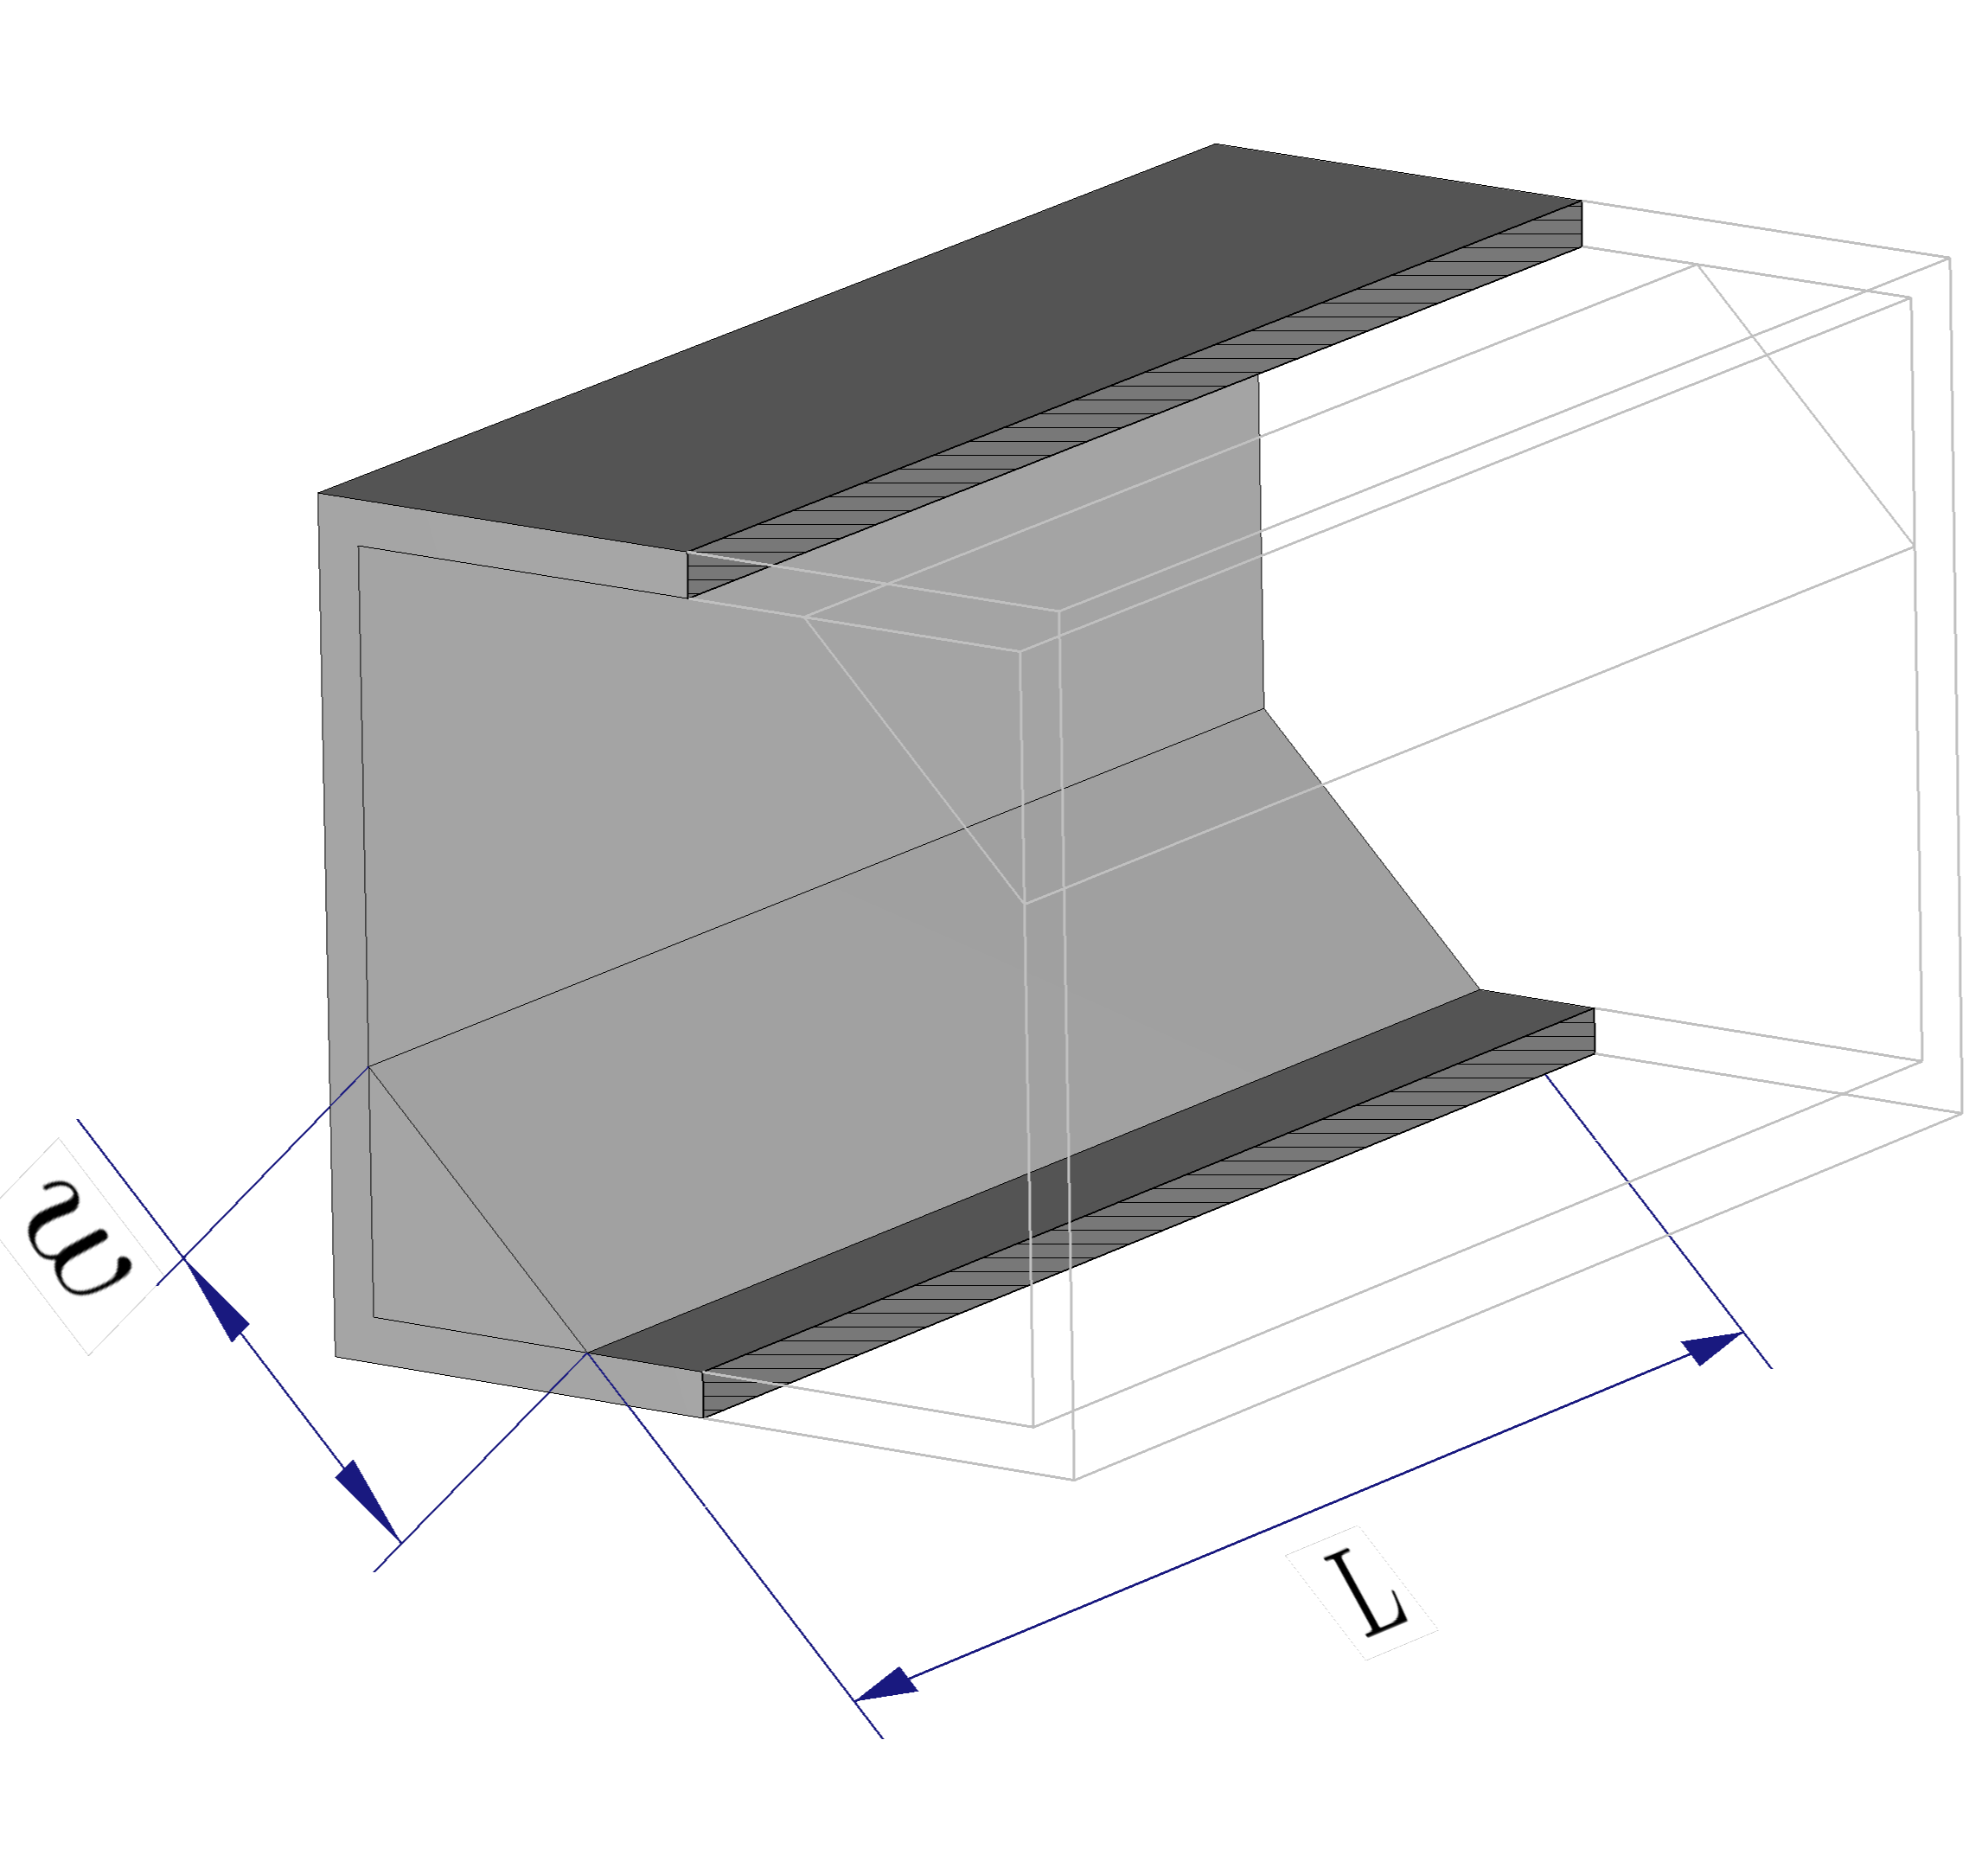
\includegraphics[width=\textwidth]{src/polarizer_square_perspective.png}
        \caption{\label{fig:polarizer-square-perspective}}
    \end{subfigure}
    \hfill
    \begin{subfigure}{.45\textwidth}
        \centering
        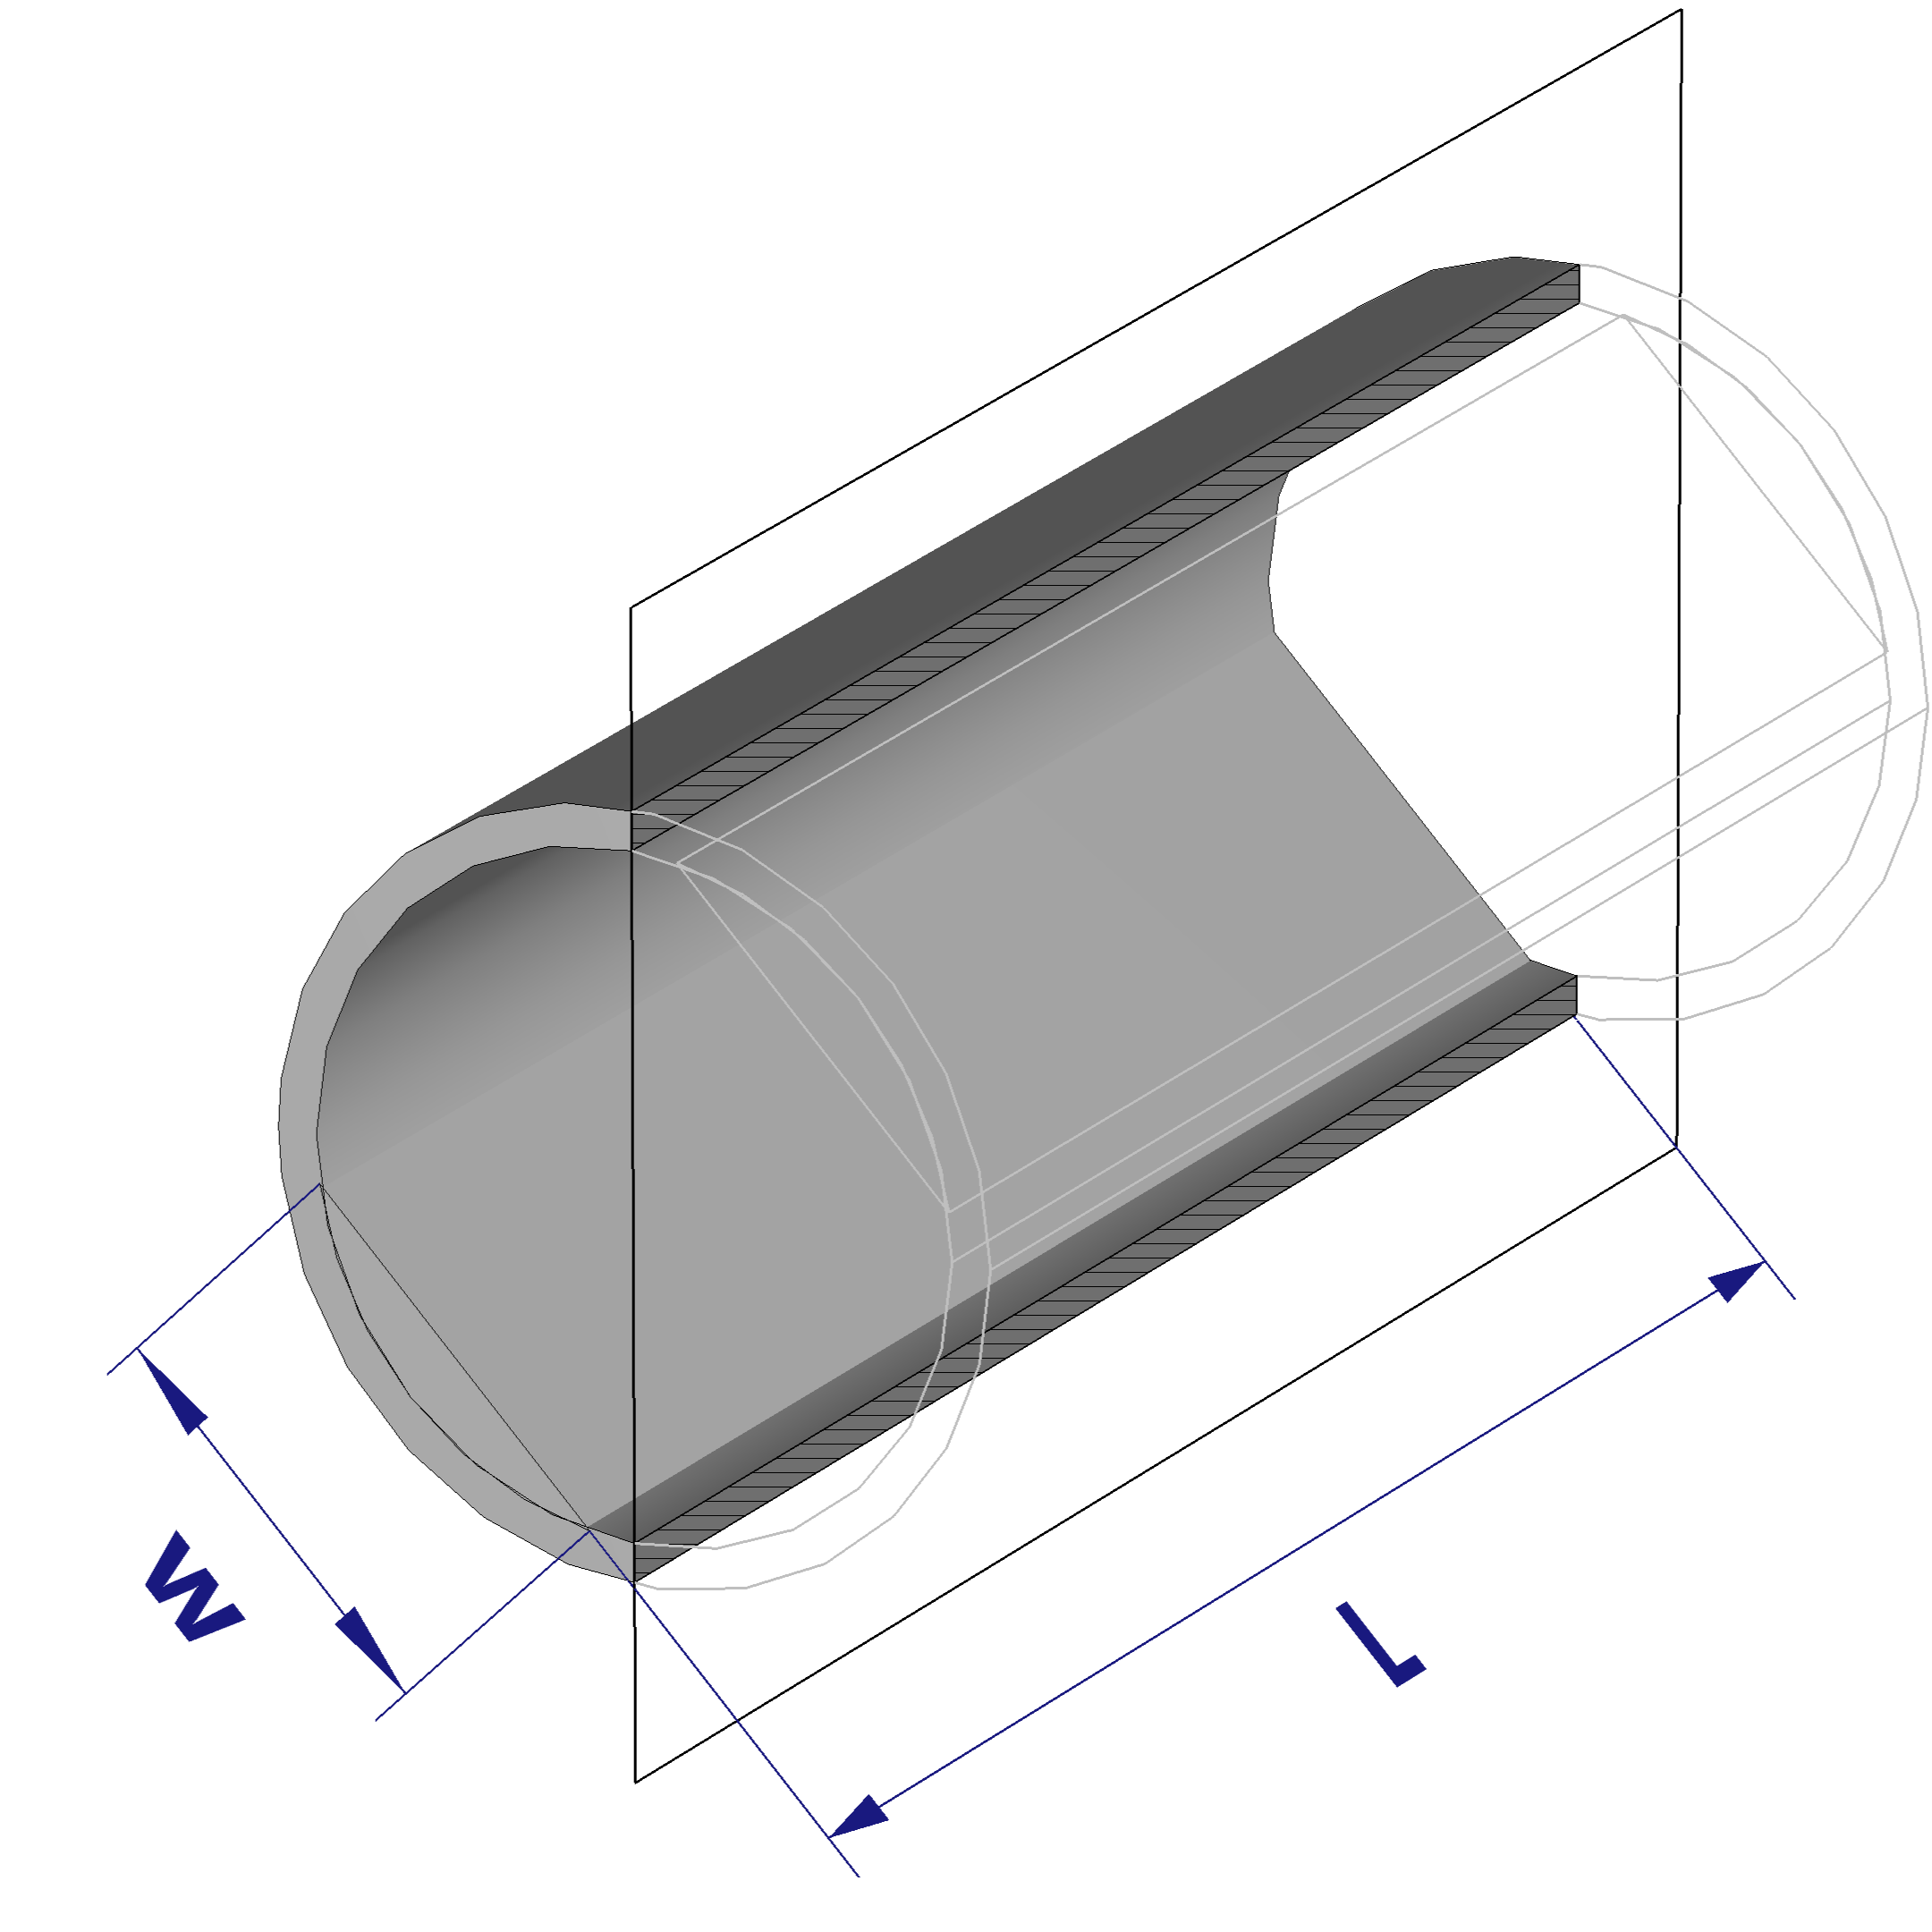
\includegraphics[width=\textwidth]{src/polarizer_circular_perspective.png}
        \caption{\label{fig:polarizer-circular-perspective}}
    \end{subfigure}
    \caption{\label{fig:polarizers}Polarizers based on symmetric waveguides}
\end{figure}

This approach was selected primarily for its relative ease of fabrication, particularly at higher frequencies, and its potential for adaptation to various frequency bands. However, due to the resonant, and hence geometry-dependent, nature of the mode dispersion introduced by the prismatic inserts, optimal performance is anticipated over a moderately wide bandwidth, rather than an ultrawide one. This bandwidth limitation represents a trade-off for the design's simplicity, robustness, and manufacturability. The use of triangular prisms, in particular, simplifies fabrication compared to more complex curved geometries while still providing effective field manipulation for polarization control.

\section{Eigenmode analysis}
The focus now shifts to the \emph{eigenmode analysis} the two waveguides illustrated in \cref{fig:polarizers}. This powerful technique, based on the theory outlined in \cref{remark:modal-decomposition-of-guided-waves}, facilitates the establishment of figures of merit intrinsic to polarizing structures, enabling performance tracking and aiding in the determination of the more advantageous geometry.

Initially, the fundamental modes of propagation in the symmetric waveguides, \emph{without} the inserted prisms, are considered. In the case of the square waveguide, it is the $\TE 10$ and $\TE 01$ modes illustrated in \cref{fig:square-waveguide-mode1,fig:square-waveguide-mode2}, whereas the two degenerate $\TE 11$ modes%
    \footnote{Note that circular waveguides posses an infinite number of degenerate $\TE 11$ modes due to their rotational symmetry. Here, two are chosen for their perpendicular oscillations which aligns well with the definition of circular polarization in \cref{subsection:polarization}.}
of the circular waveguide are presented in \cref{fig:circular-waveguide-mode1,fig:circular-waveguide-mode2}. For both waveguides individually, these two degenerate modes represent the two waves launched into the polarizer via a section of standard waveguide. Upon encountering the metallic inserts, such incident wave no longer represents the eigenmode of the simple waveguide structure and its energy is coupled into a linear combination of the fundamental eigenmodes of the respective polarizer.

\begin{figure}[!ht]
    \centering
    \begin{subfigure}{.45\textwidth}
        \centering
        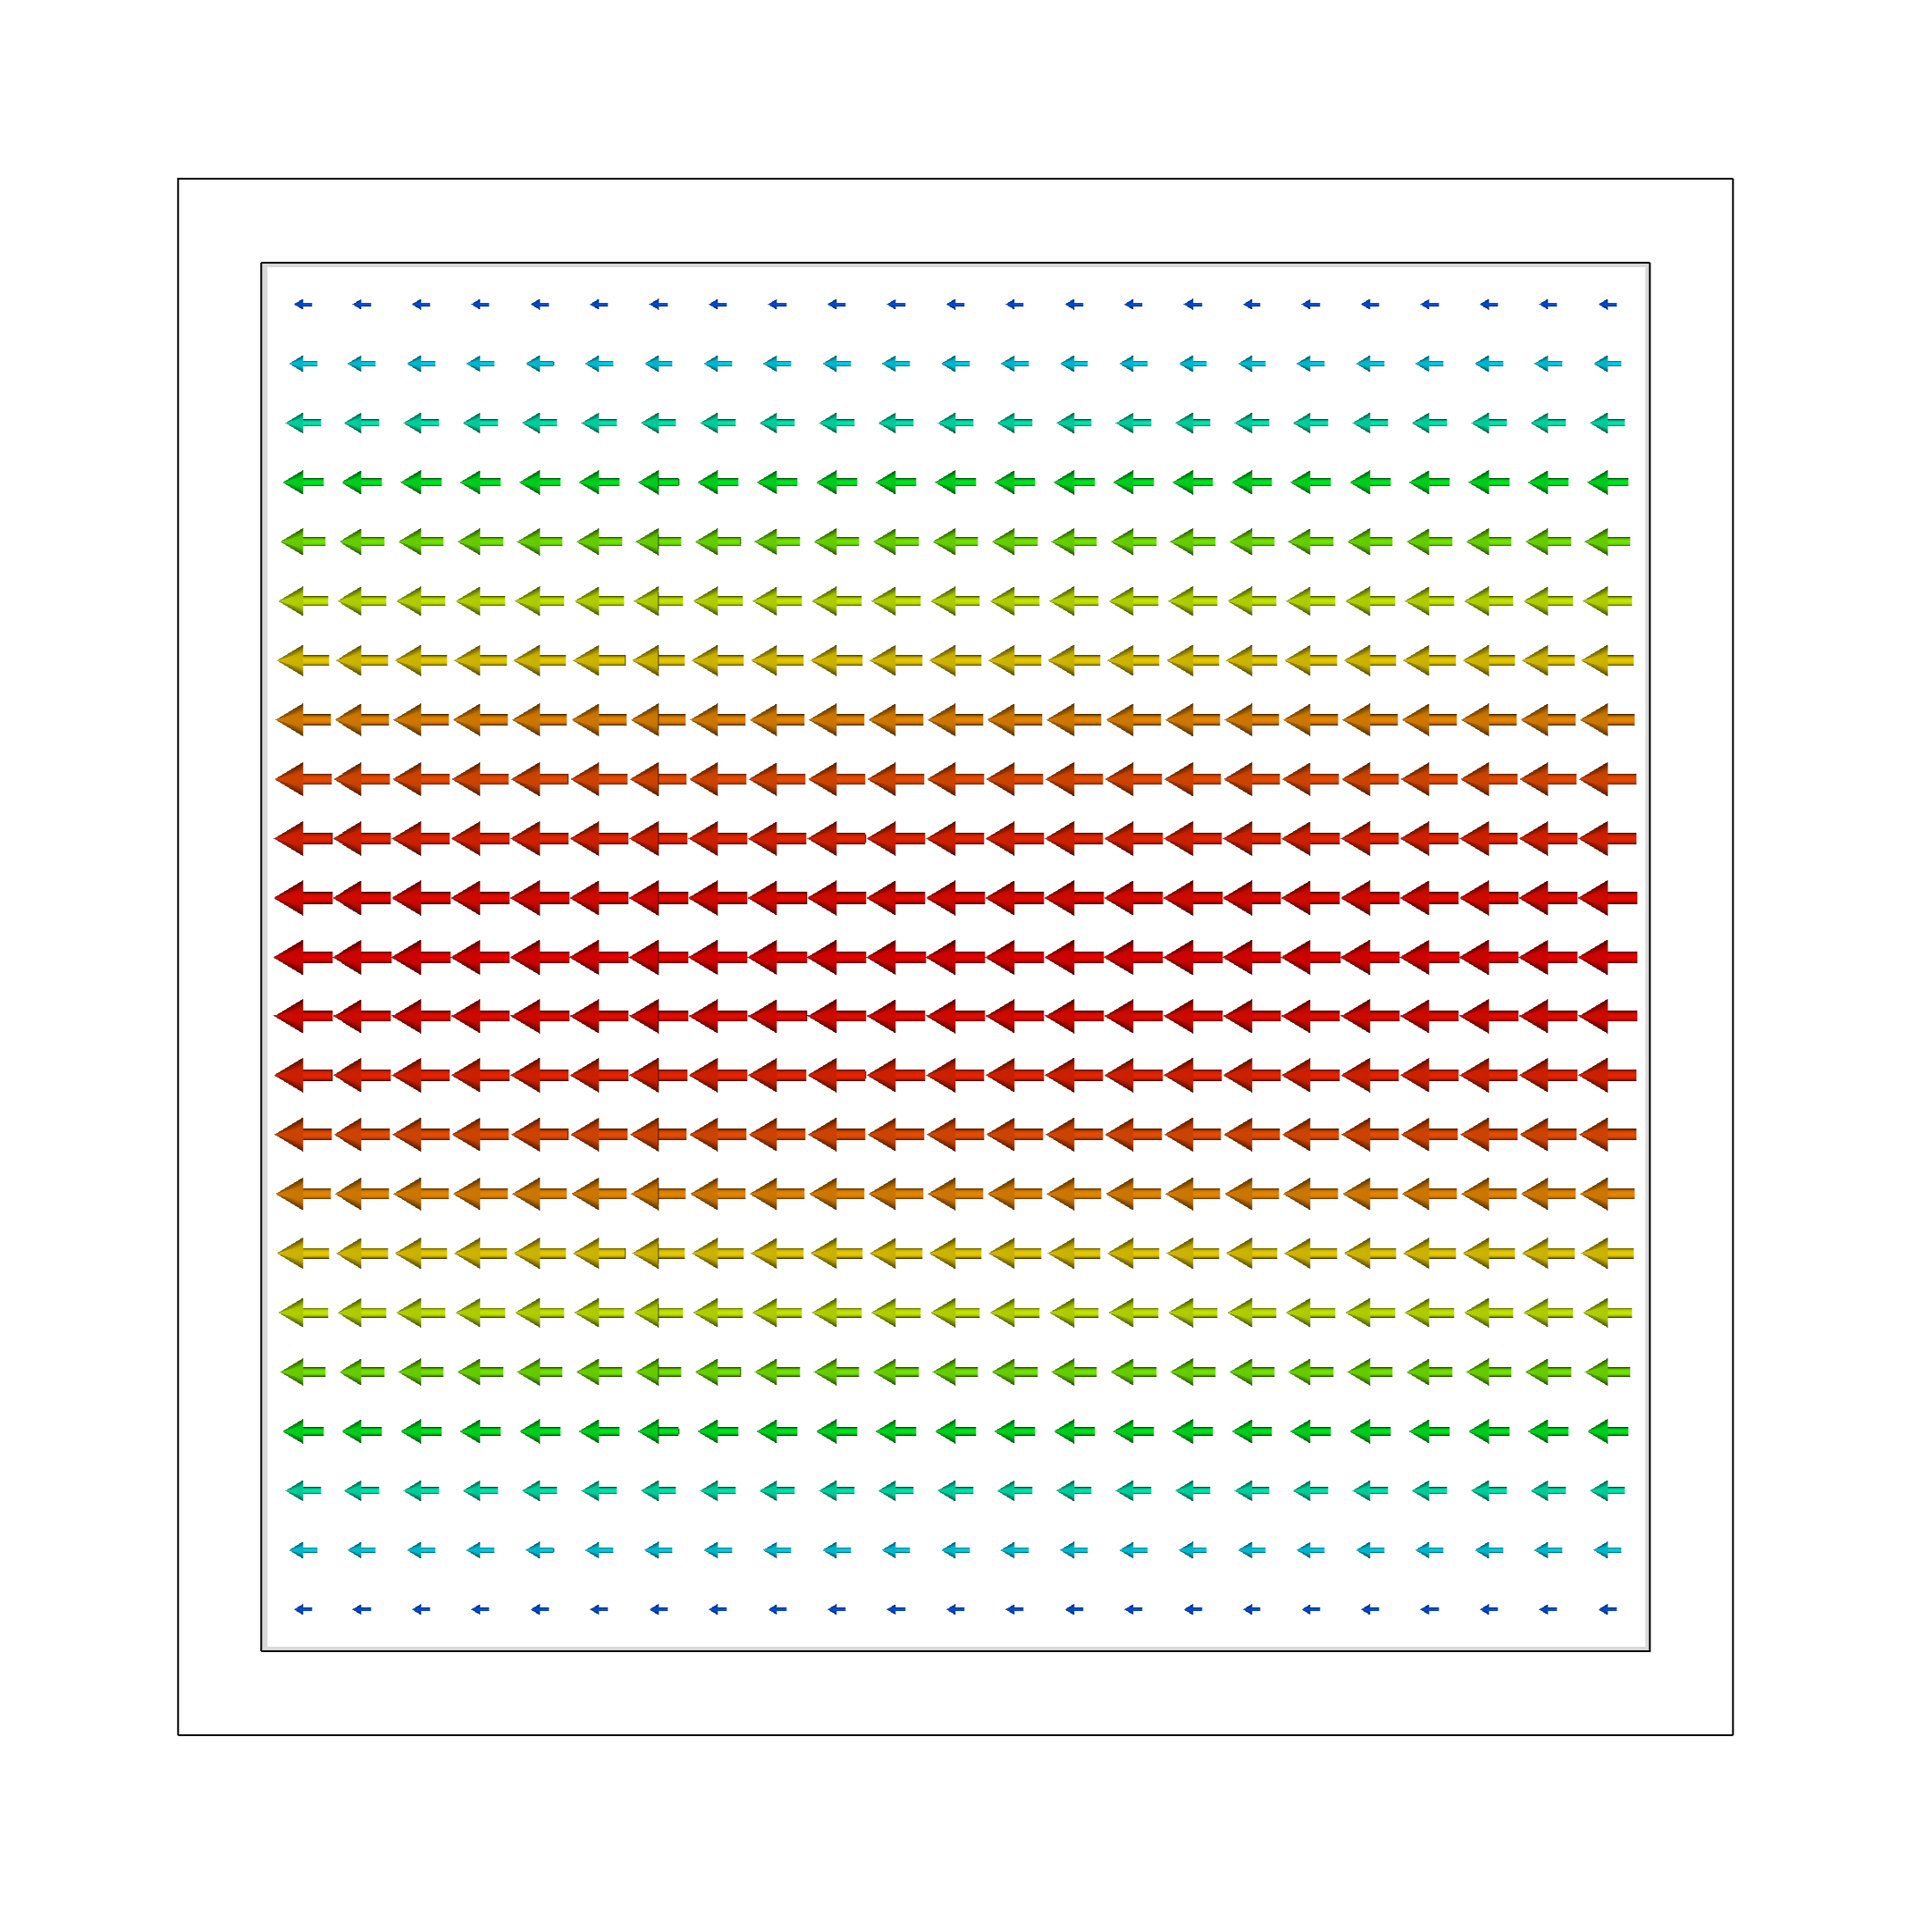
\includegraphics[width=.75\textwidth]{src/waveguide_square_mode1.png}
        \caption{\label{fig:square-waveguide-mode1}}
    \end{subfigure}
    \hspace{0.5cm}
    \begin{subfigure}{.45\textwidth}
        \centering
        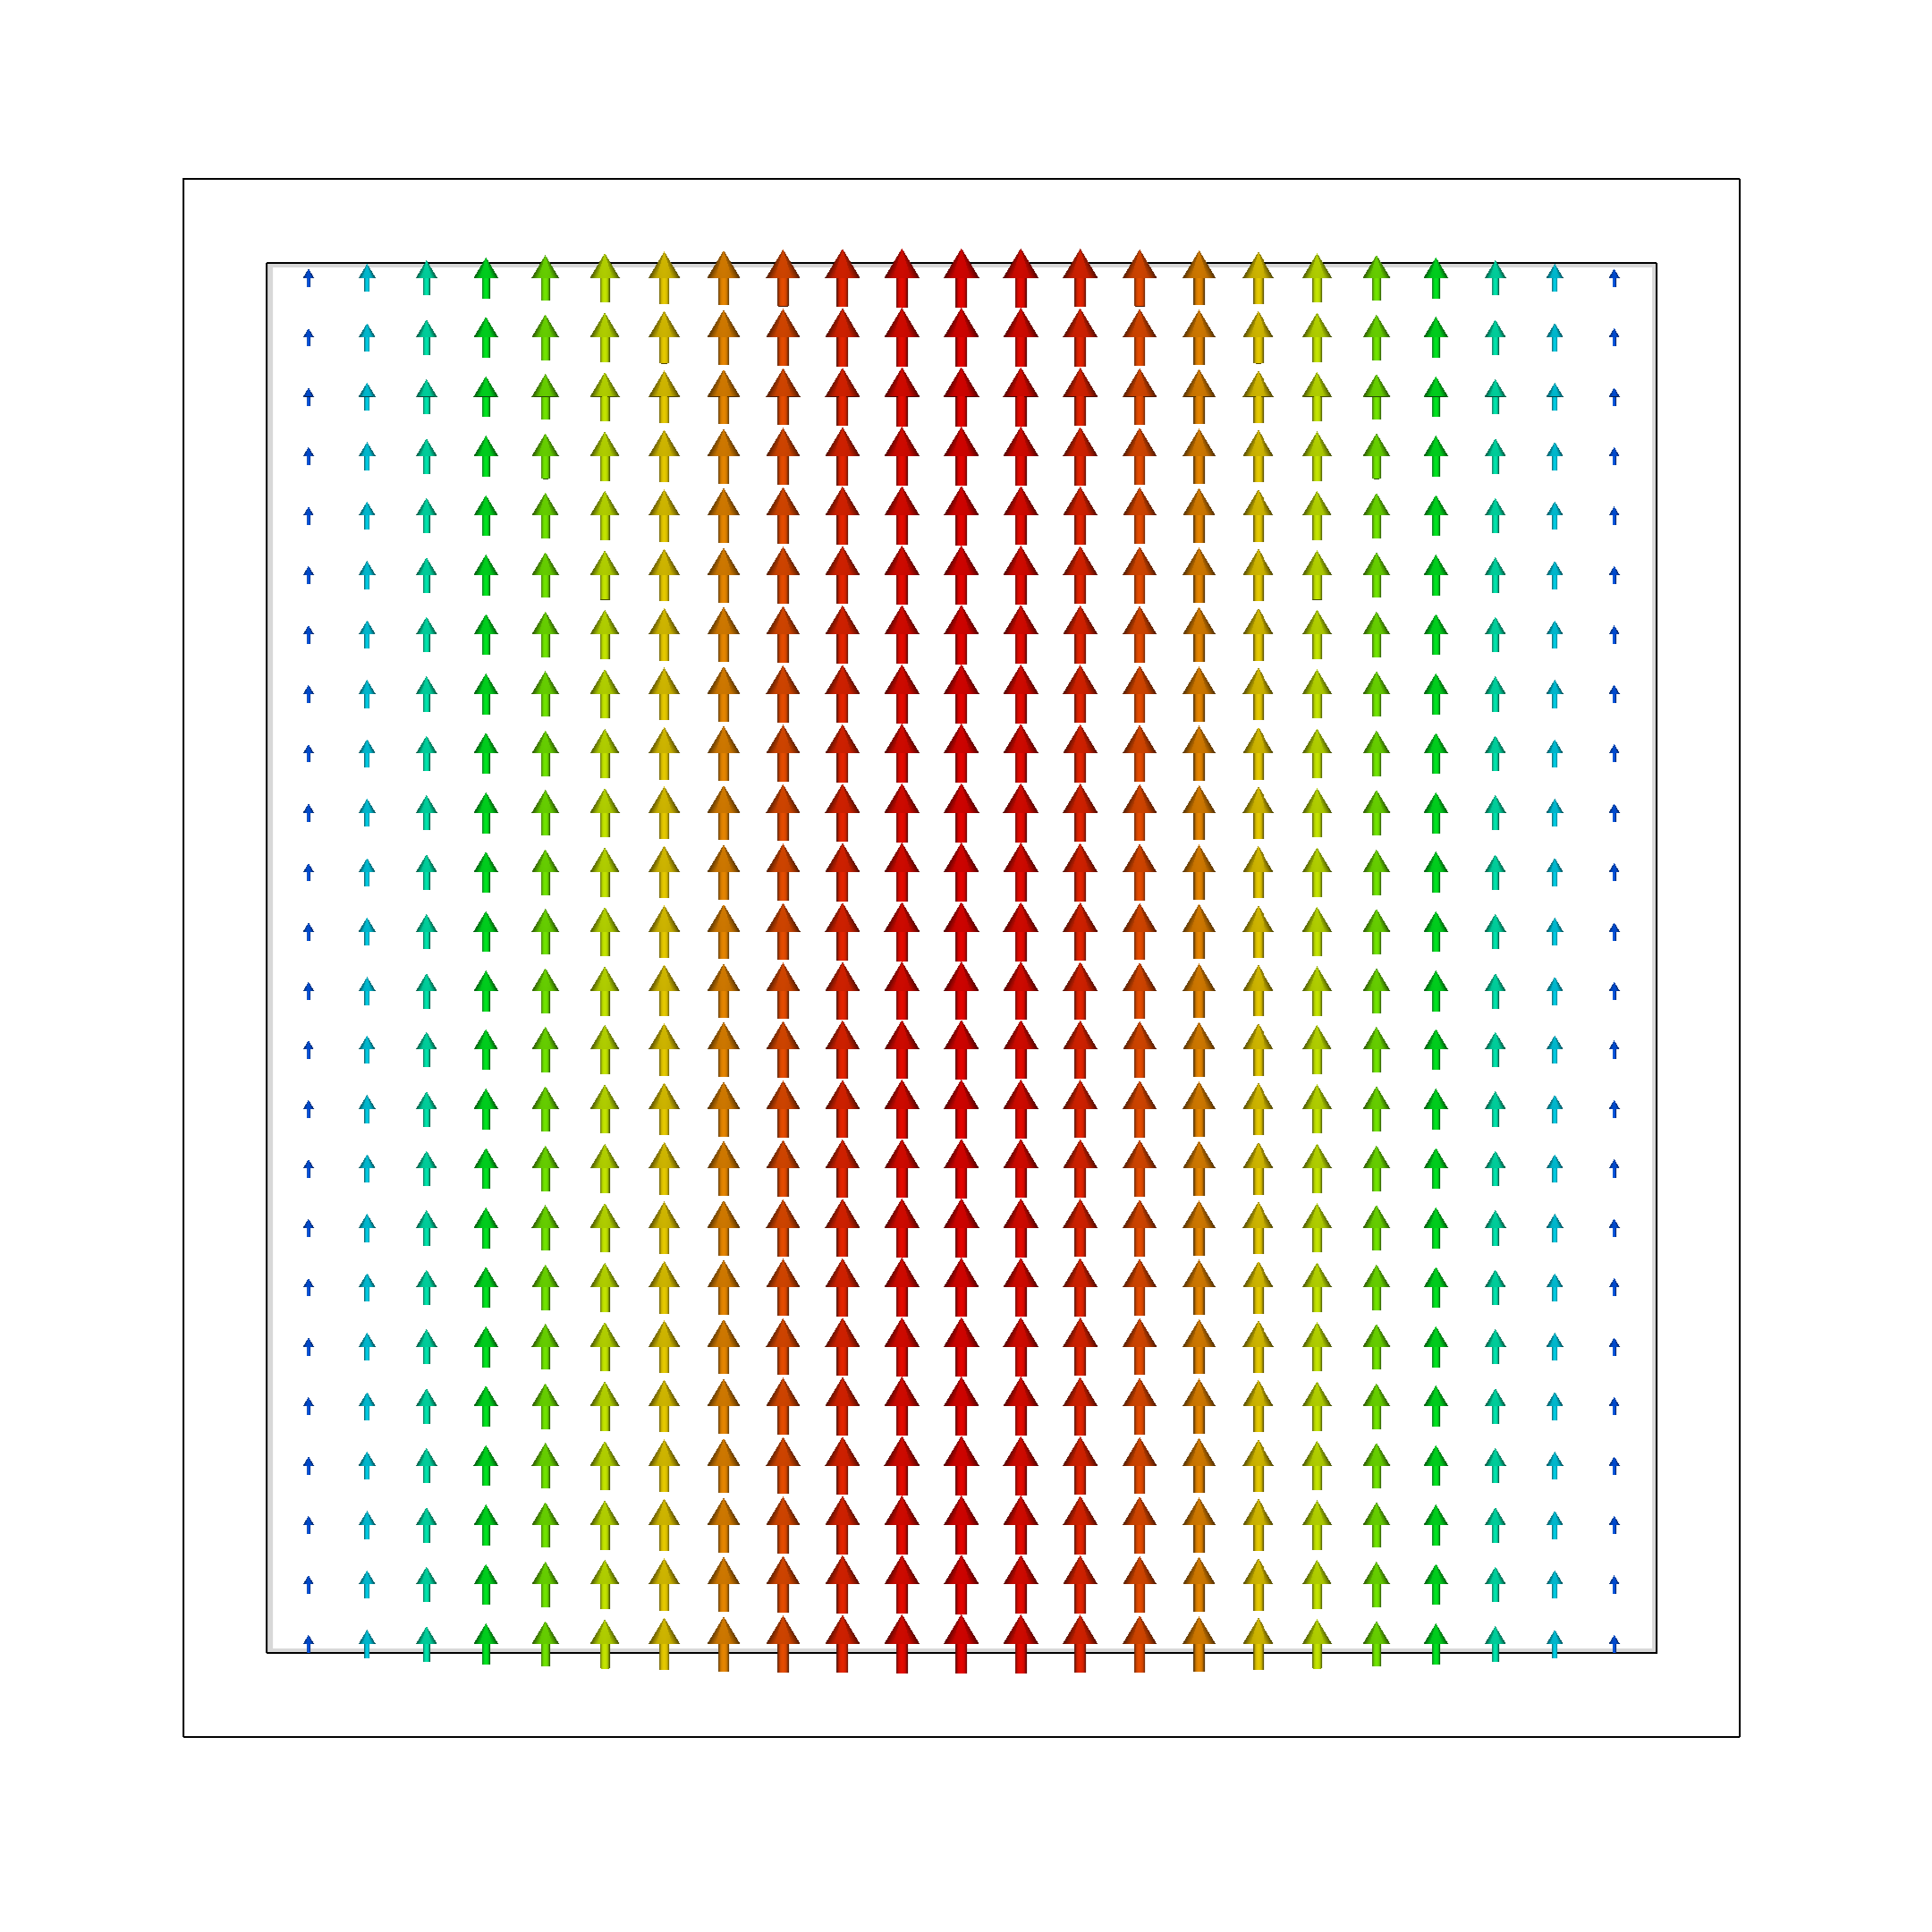
\includegraphics[width=.75\textwidth]{src/waveguide_square_mode2.png}
        \caption{\label{fig:square-waveguide-mode2}}
    \end{subfigure}
    \\
    \begin{subfigure}{.45\textwidth}
        \centering
        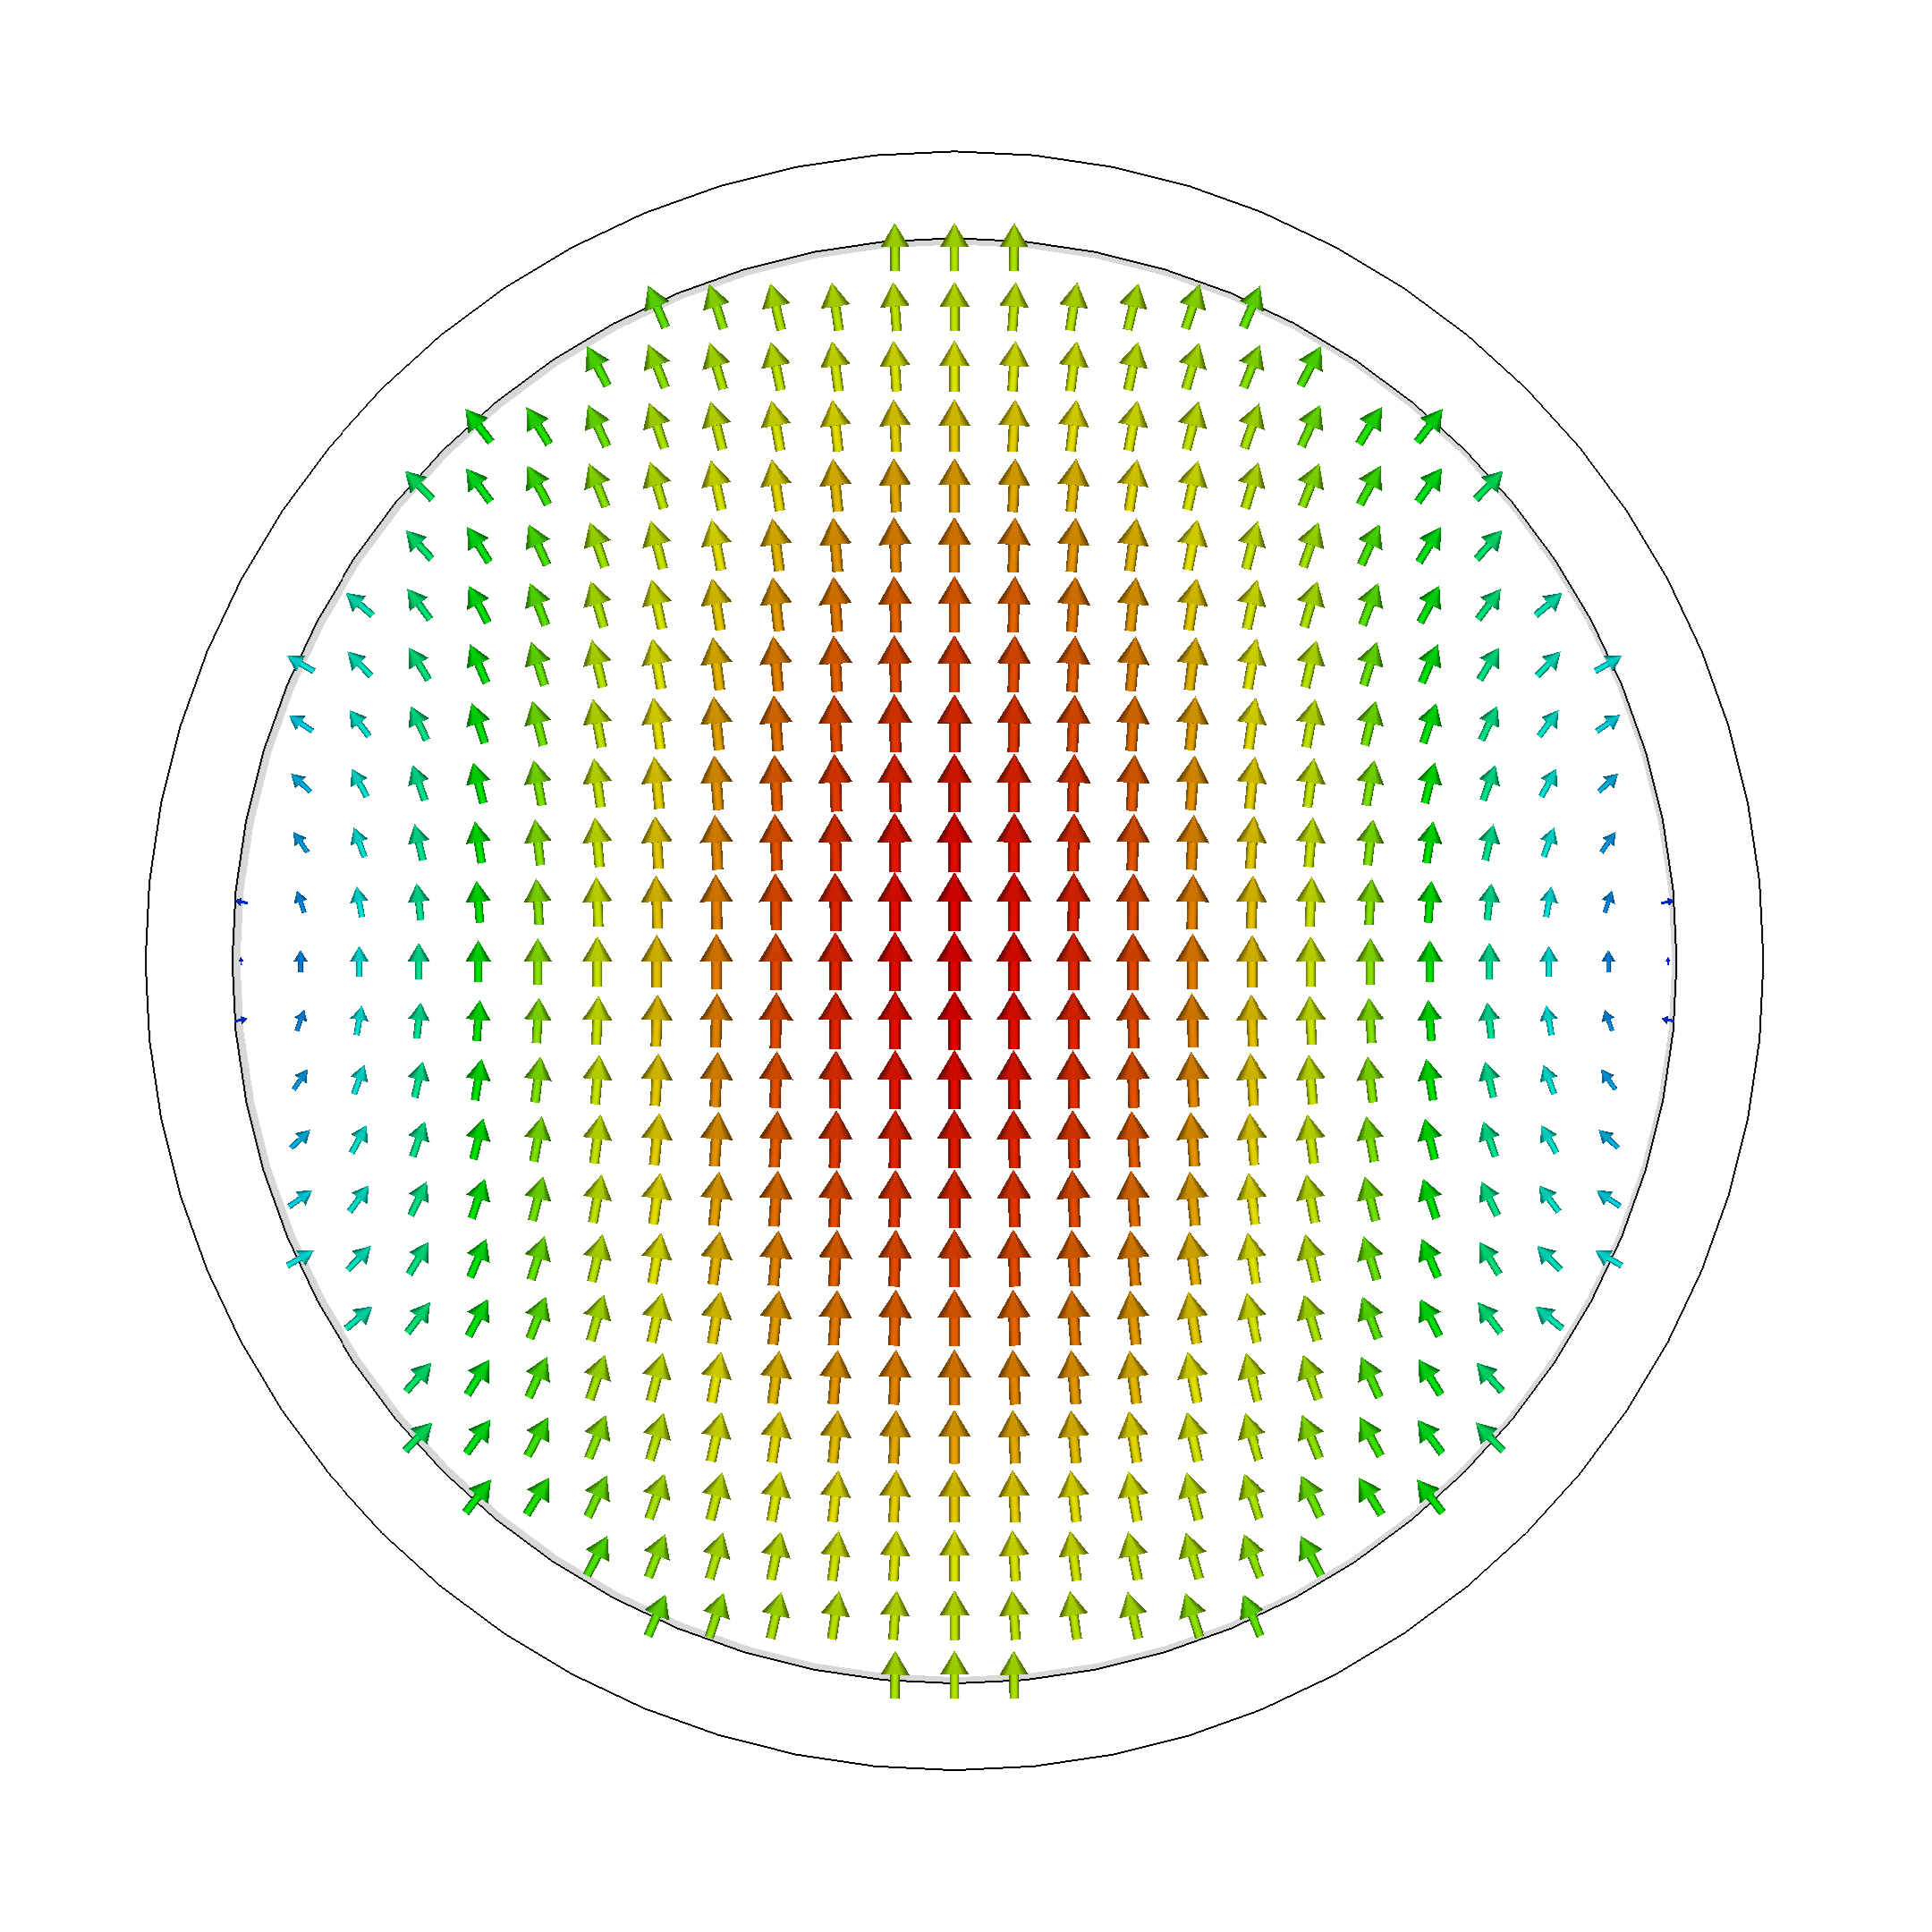
\includegraphics[width=.75\textwidth]{src/waveguide_circular_mode1.png}
        \caption{\label{fig:circular-waveguide-mode1}}
    \end{subfigure}
    \hspace{0.5cm}
    \begin{subfigure}{.45\textwidth}
        \centering
        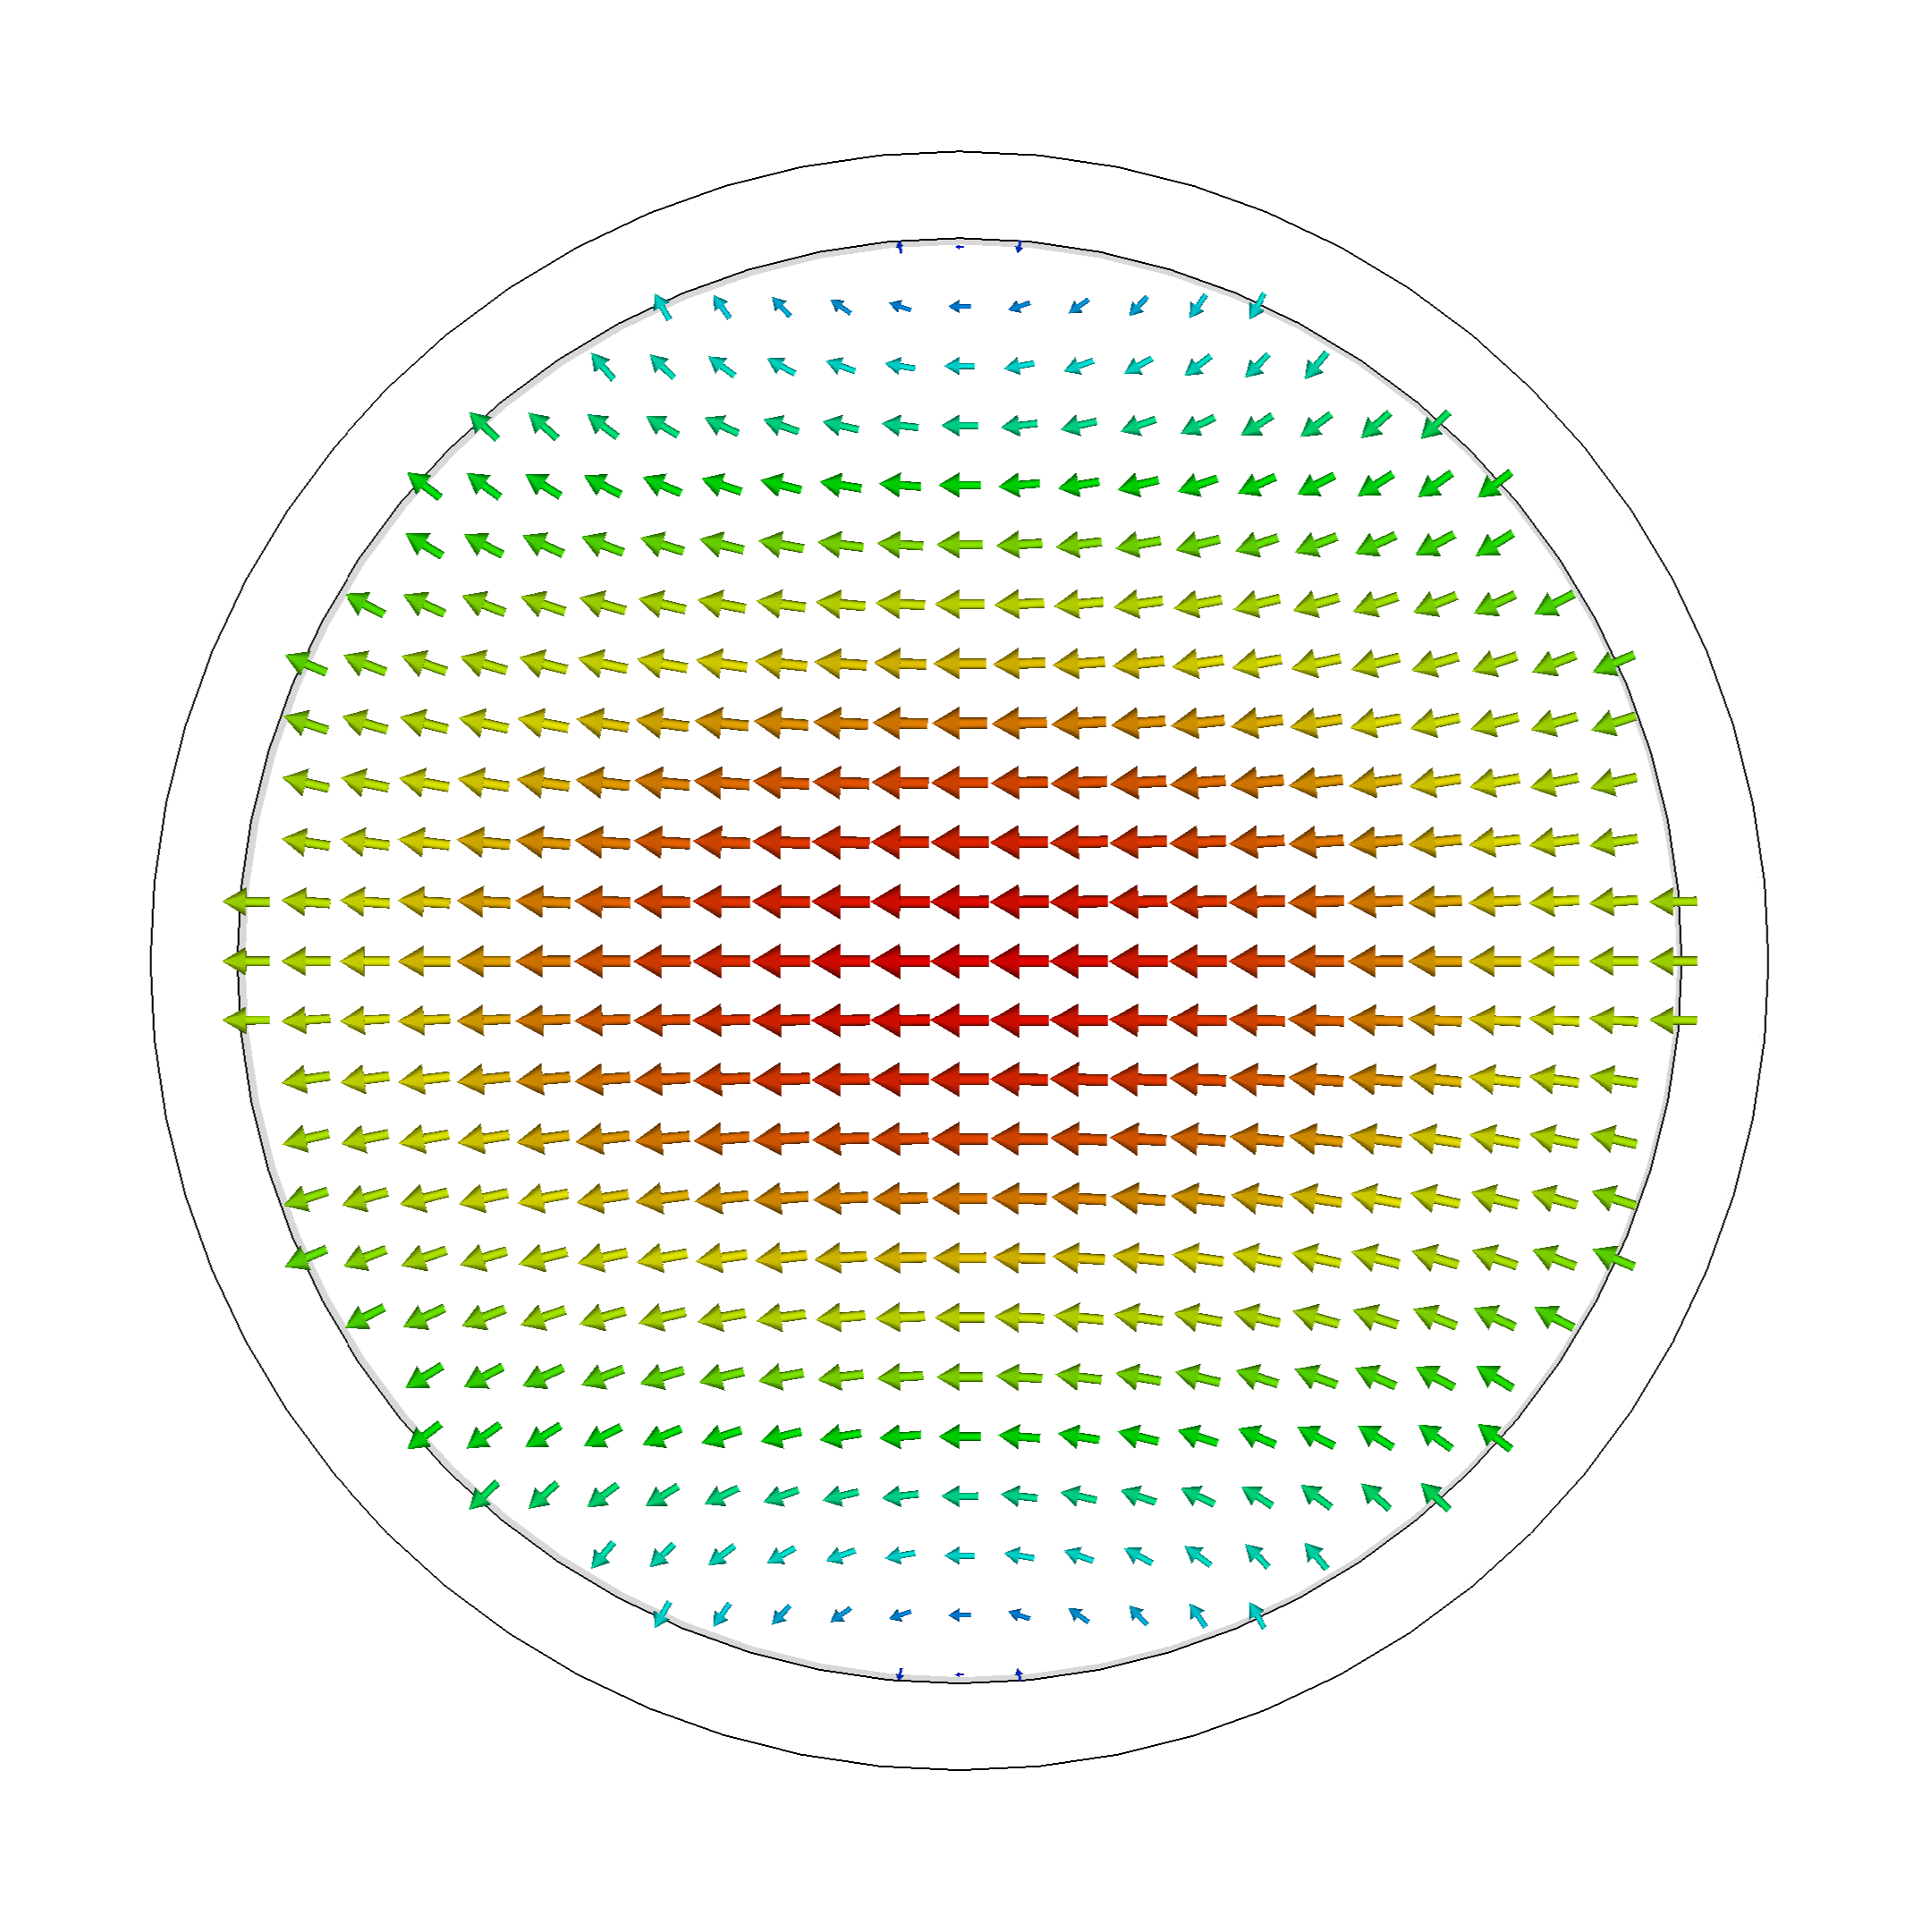
\includegraphics[width=.75\textwidth]{src/waveguide_circular_mode2.png}
        \caption{\label{fig:circular-waveguide-mode2}}
    \end{subfigure}
    \caption{\label{fig:symmetric-waveguide-modes}Fundamental modes of the symmetric waveguides}
\end{figure}

\begin{figure}[!ht]
    \centering
    \begin{subfigure}{.45\textwidth}
        \centering
        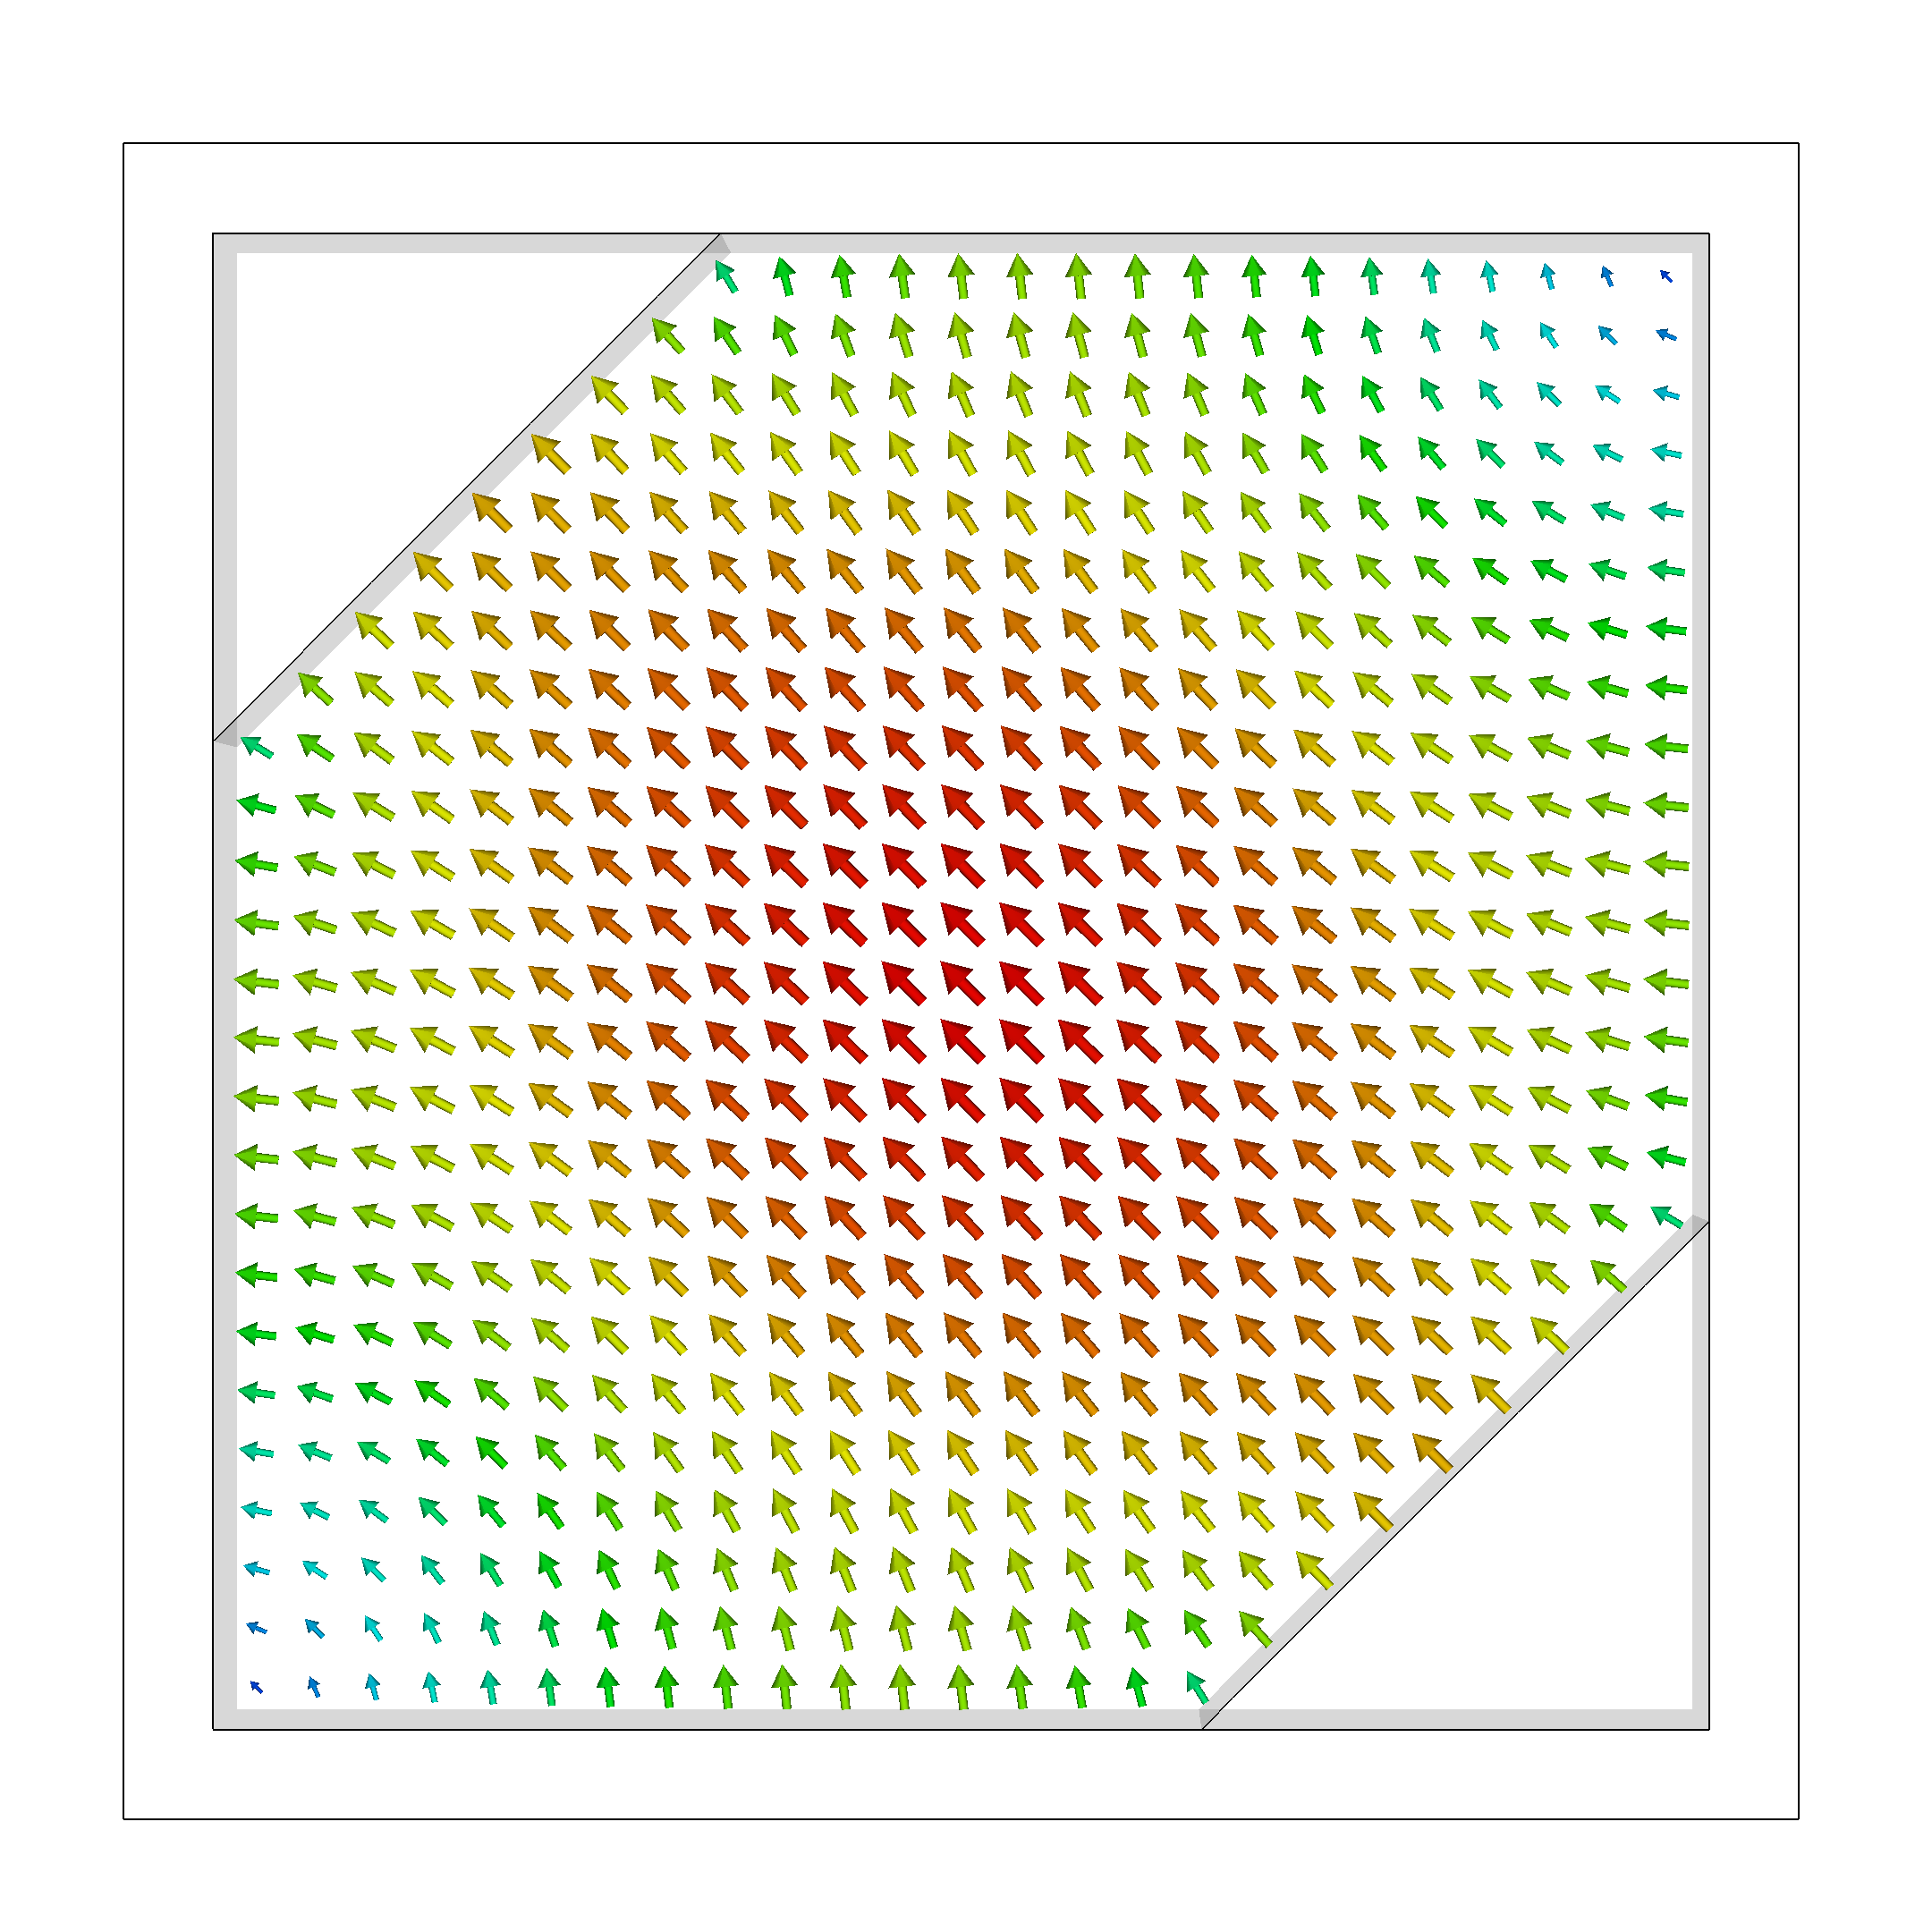
\includegraphics[width=.7\textwidth]{src/polarizer_square_mode1.png}
        \caption{\label{fig:square-polarizer-mode1}}
    \end{subfigure}
    \hspace{0.5cm}
    \begin{subfigure}{.45\textwidth}
        \centering
        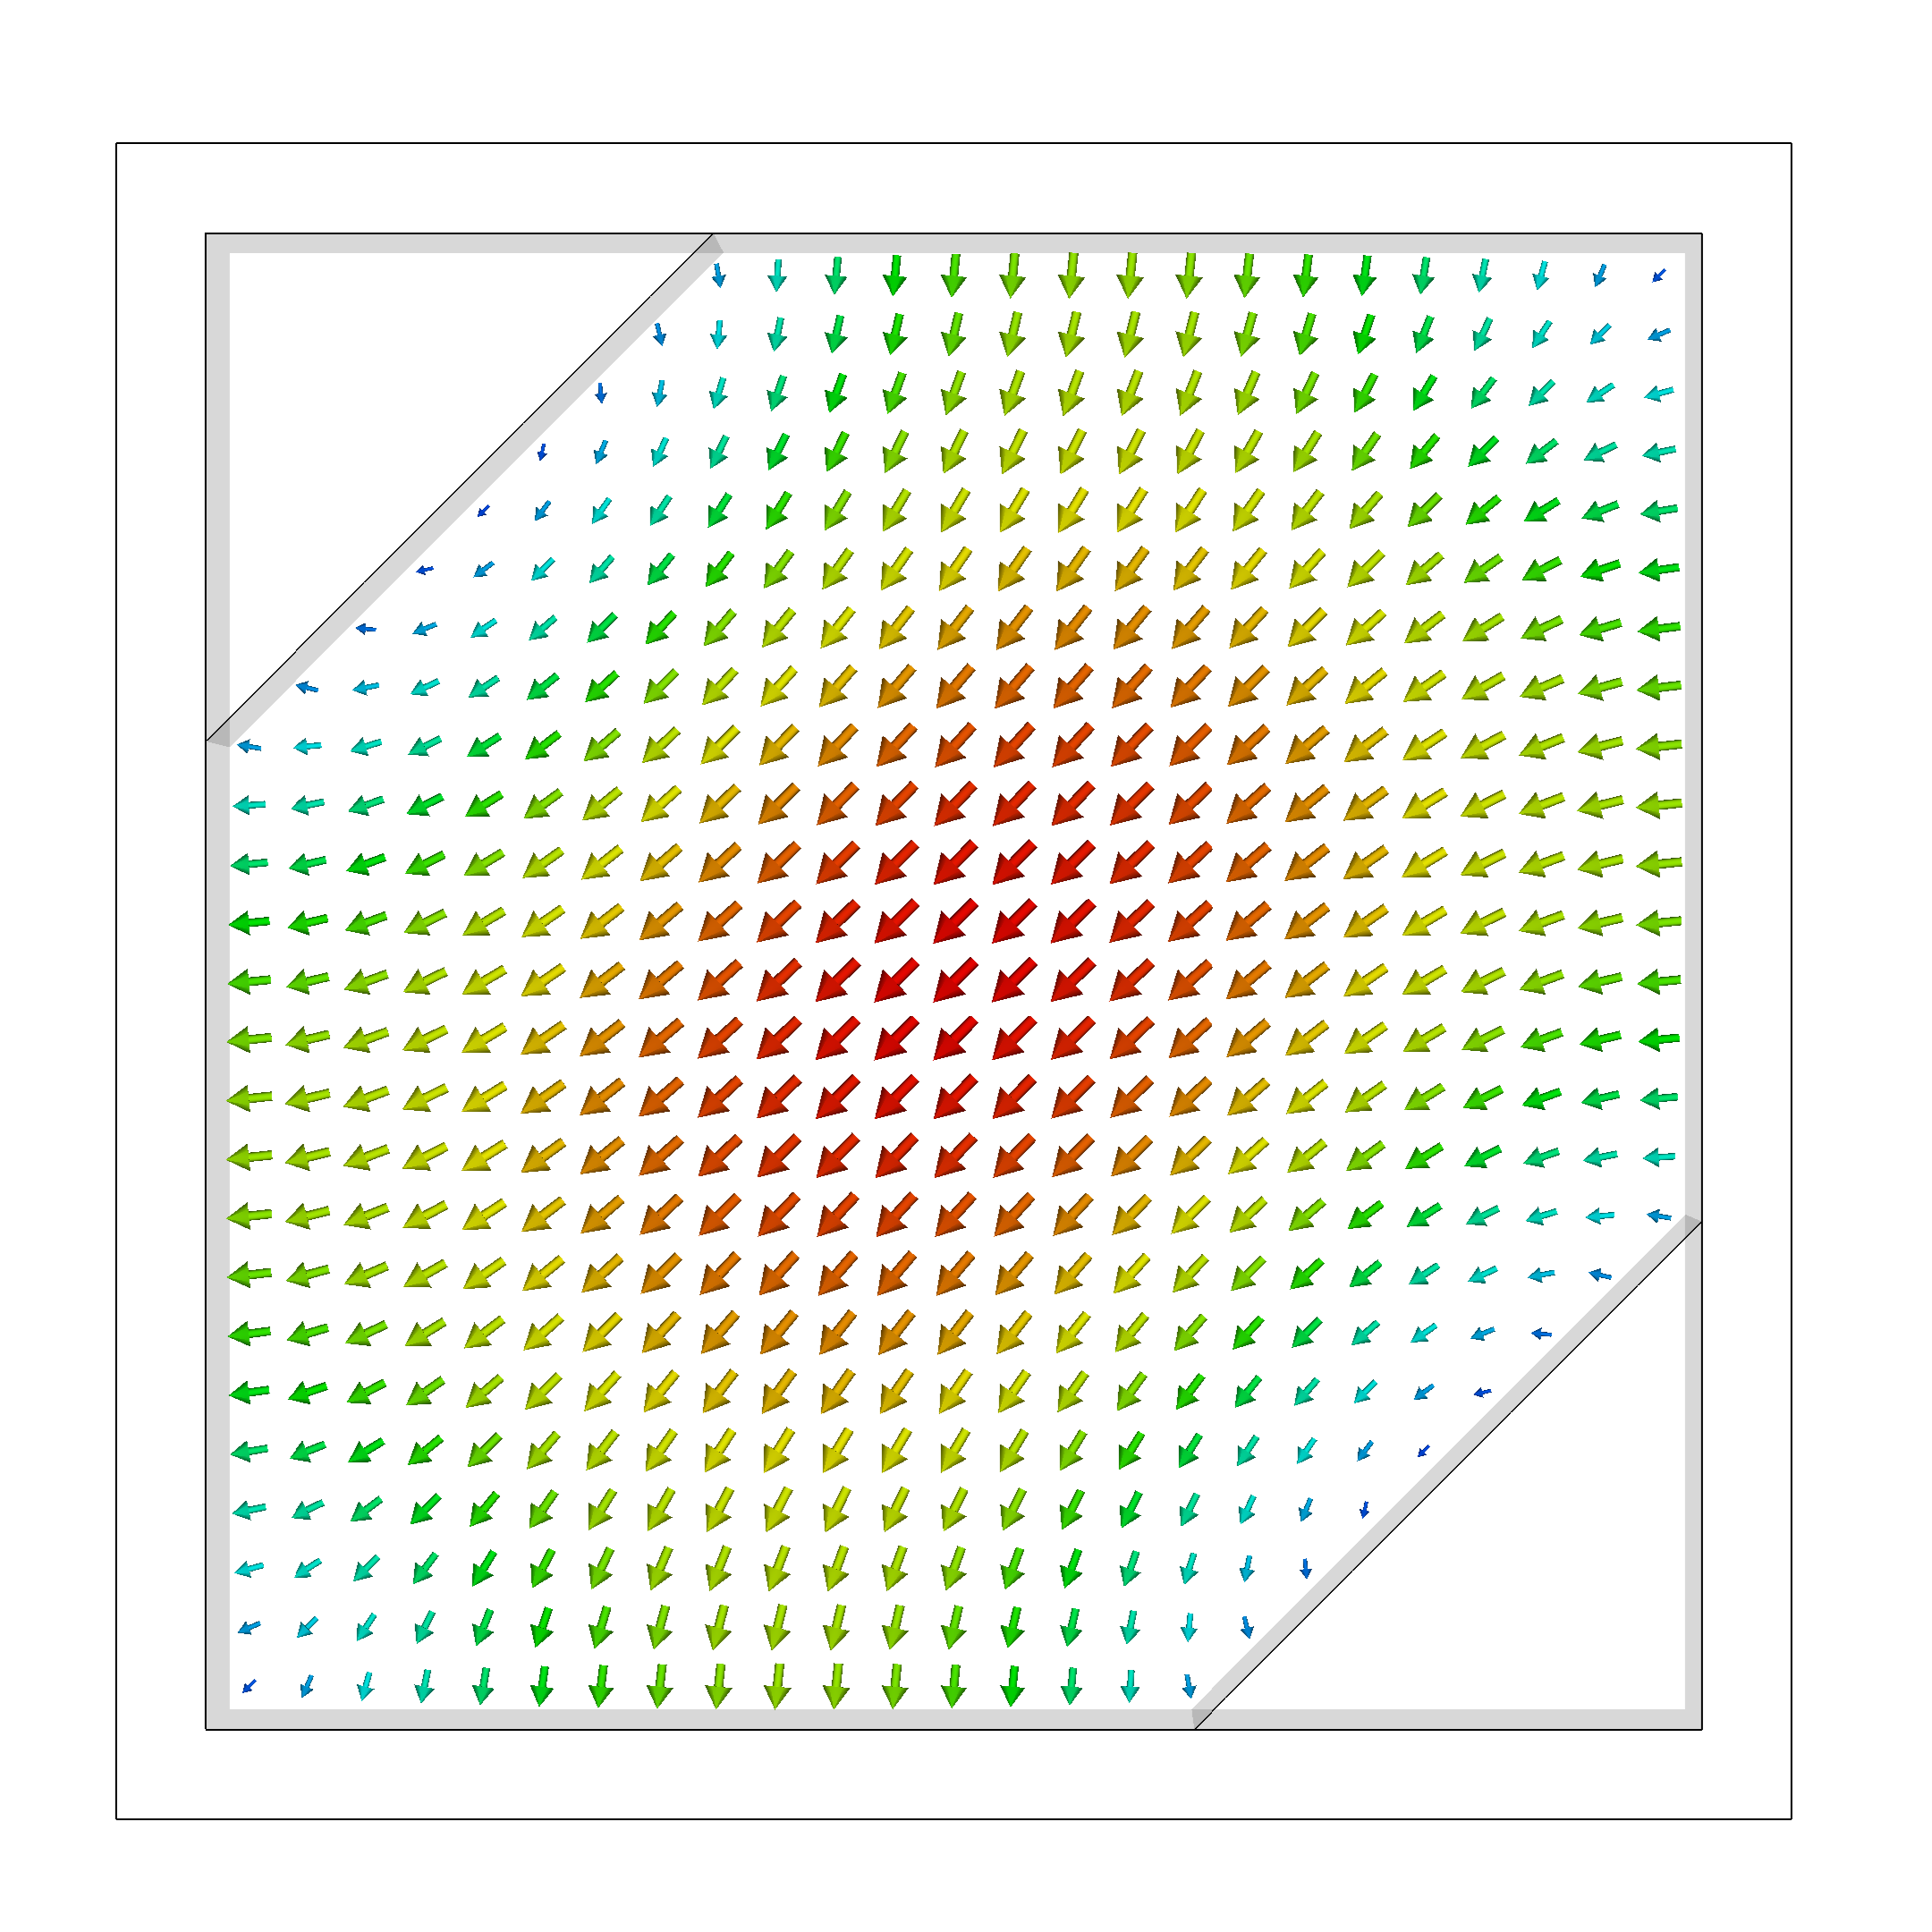
\includegraphics[width=.7\textwidth]{src/polarizer_square_mode2.png}
        \caption{\label{fig:square-polarizer-mode2}}
    \end{subfigure}
    \\
    \begin{subfigure}{.45\textwidth}
        \centering
        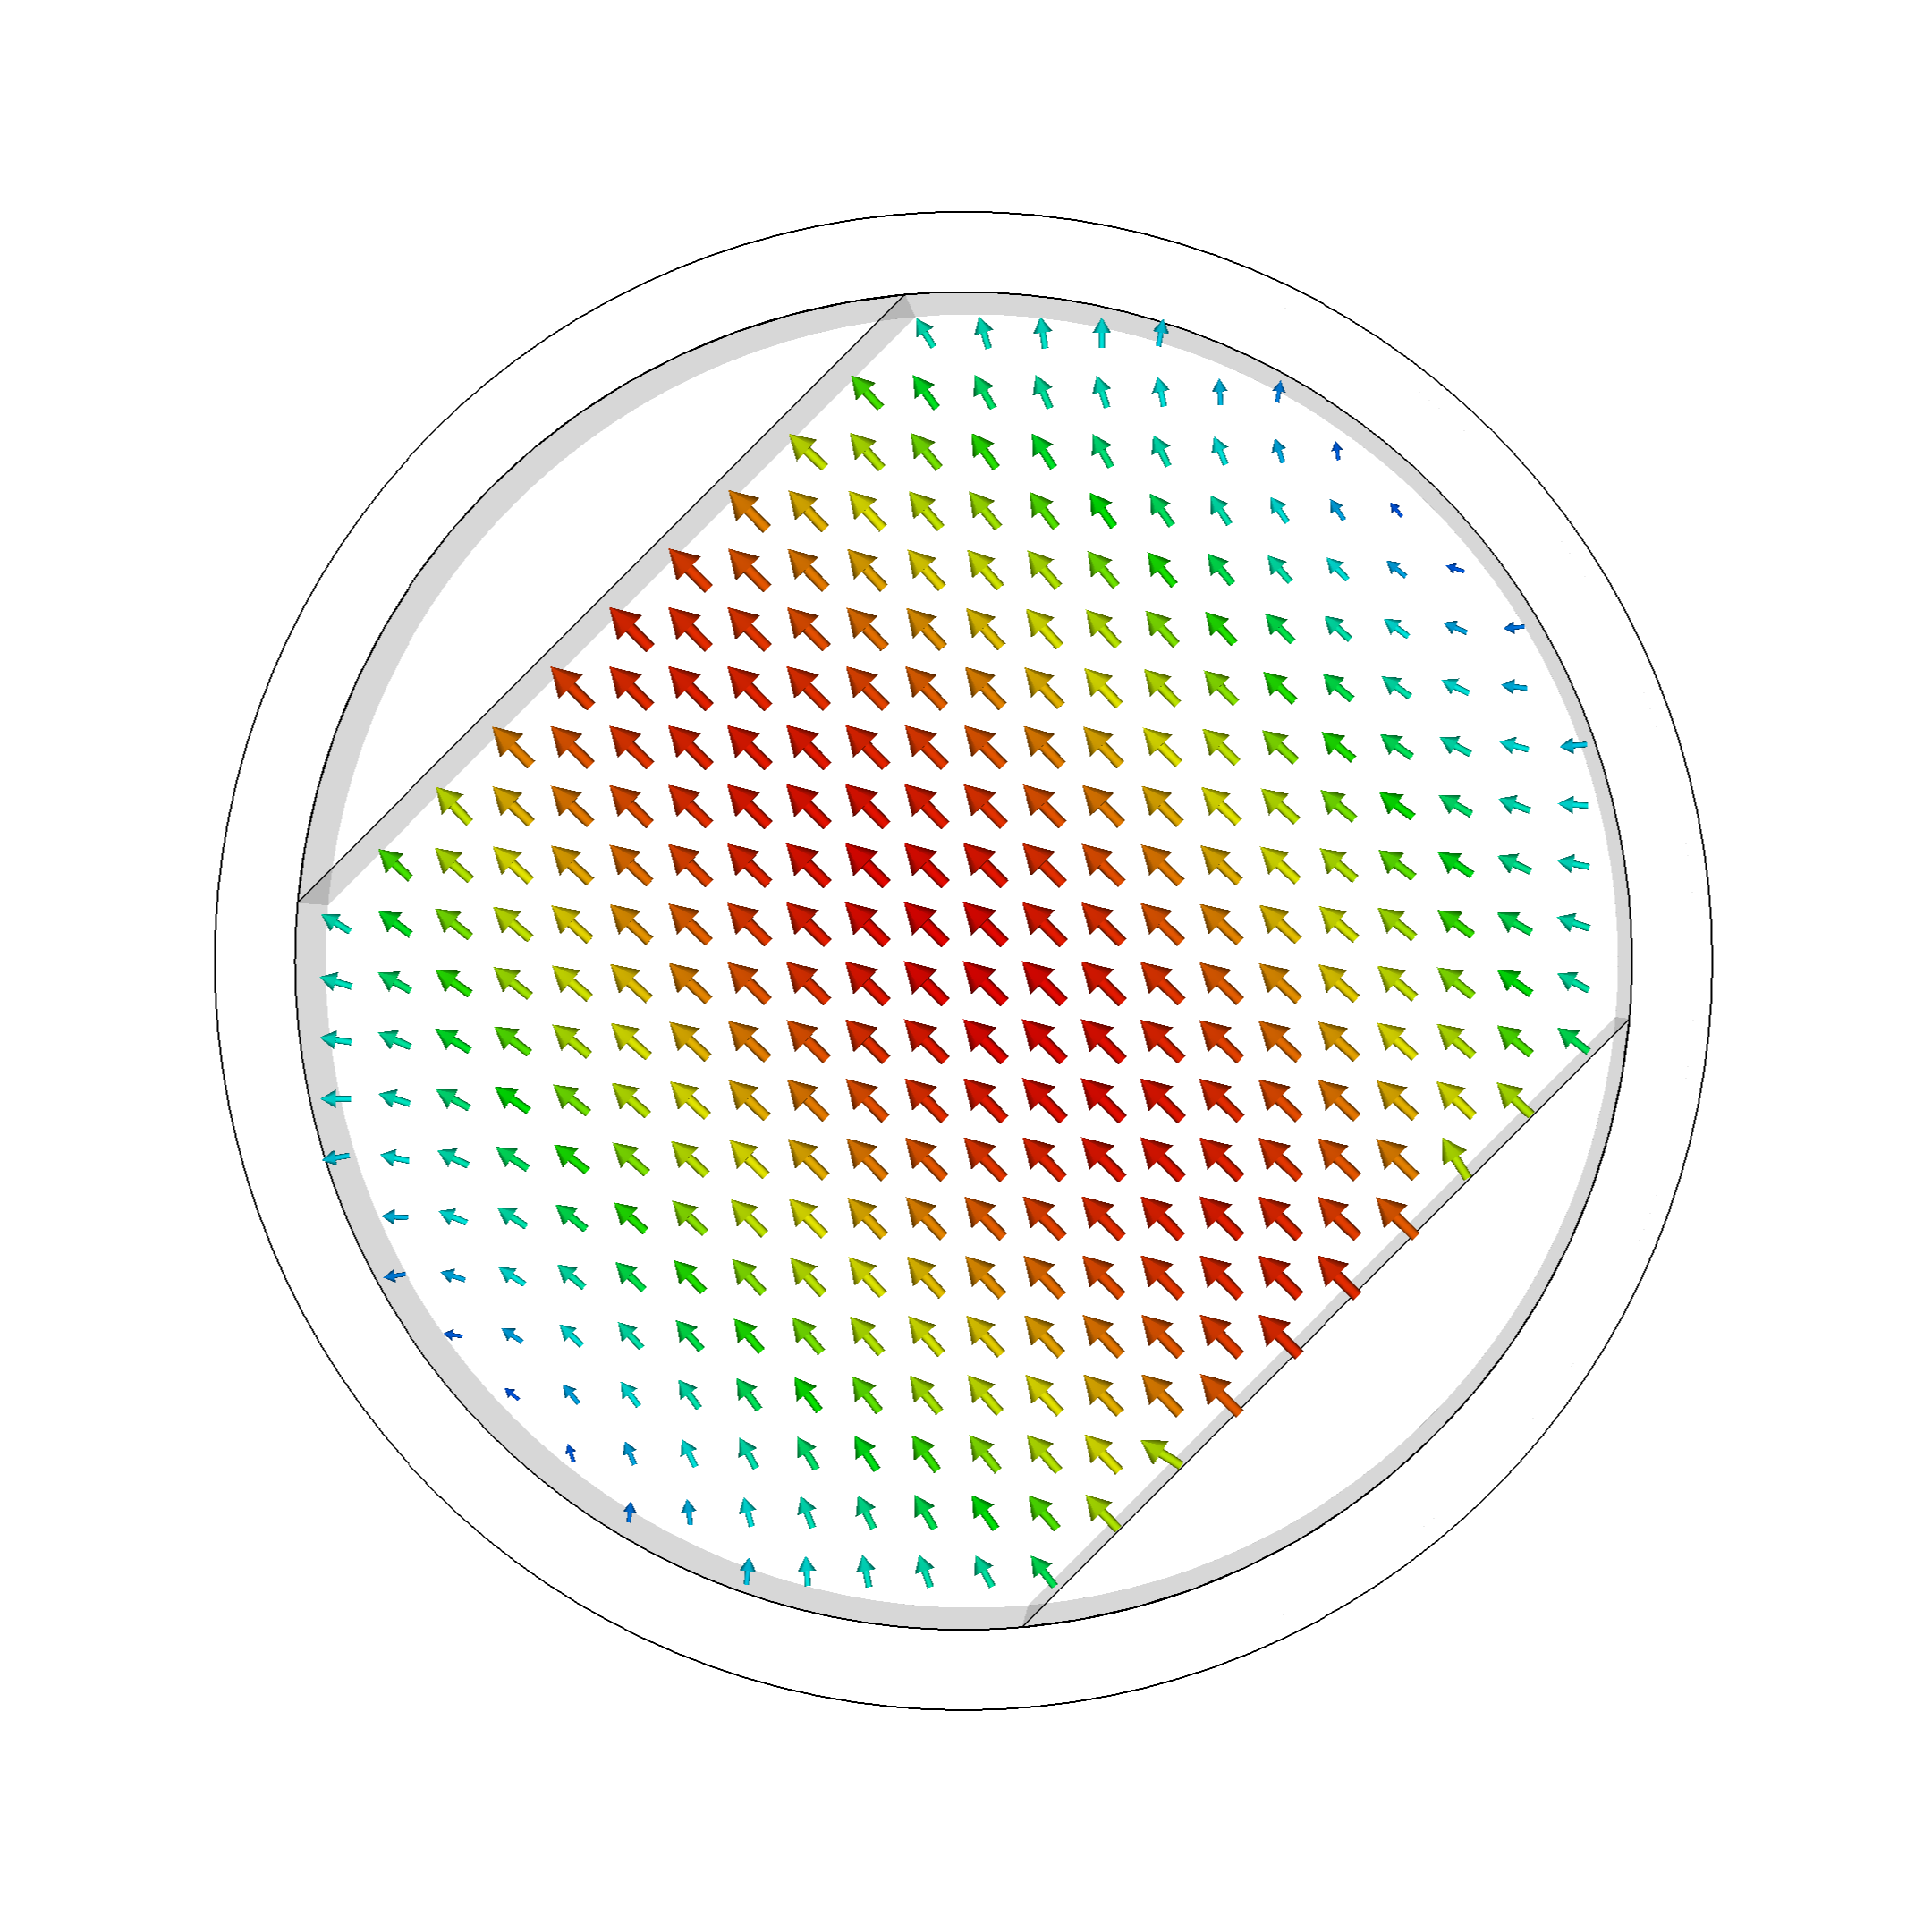
\includegraphics[width=.75\textwidth]{src/polarizer_circular_mode1.png}
        \caption{\label{fig:circular-polarizer-mode1}}
    \end{subfigure}
    \hspace{0.5cm}
    \begin{subfigure}{.45\textwidth}
        \centering
        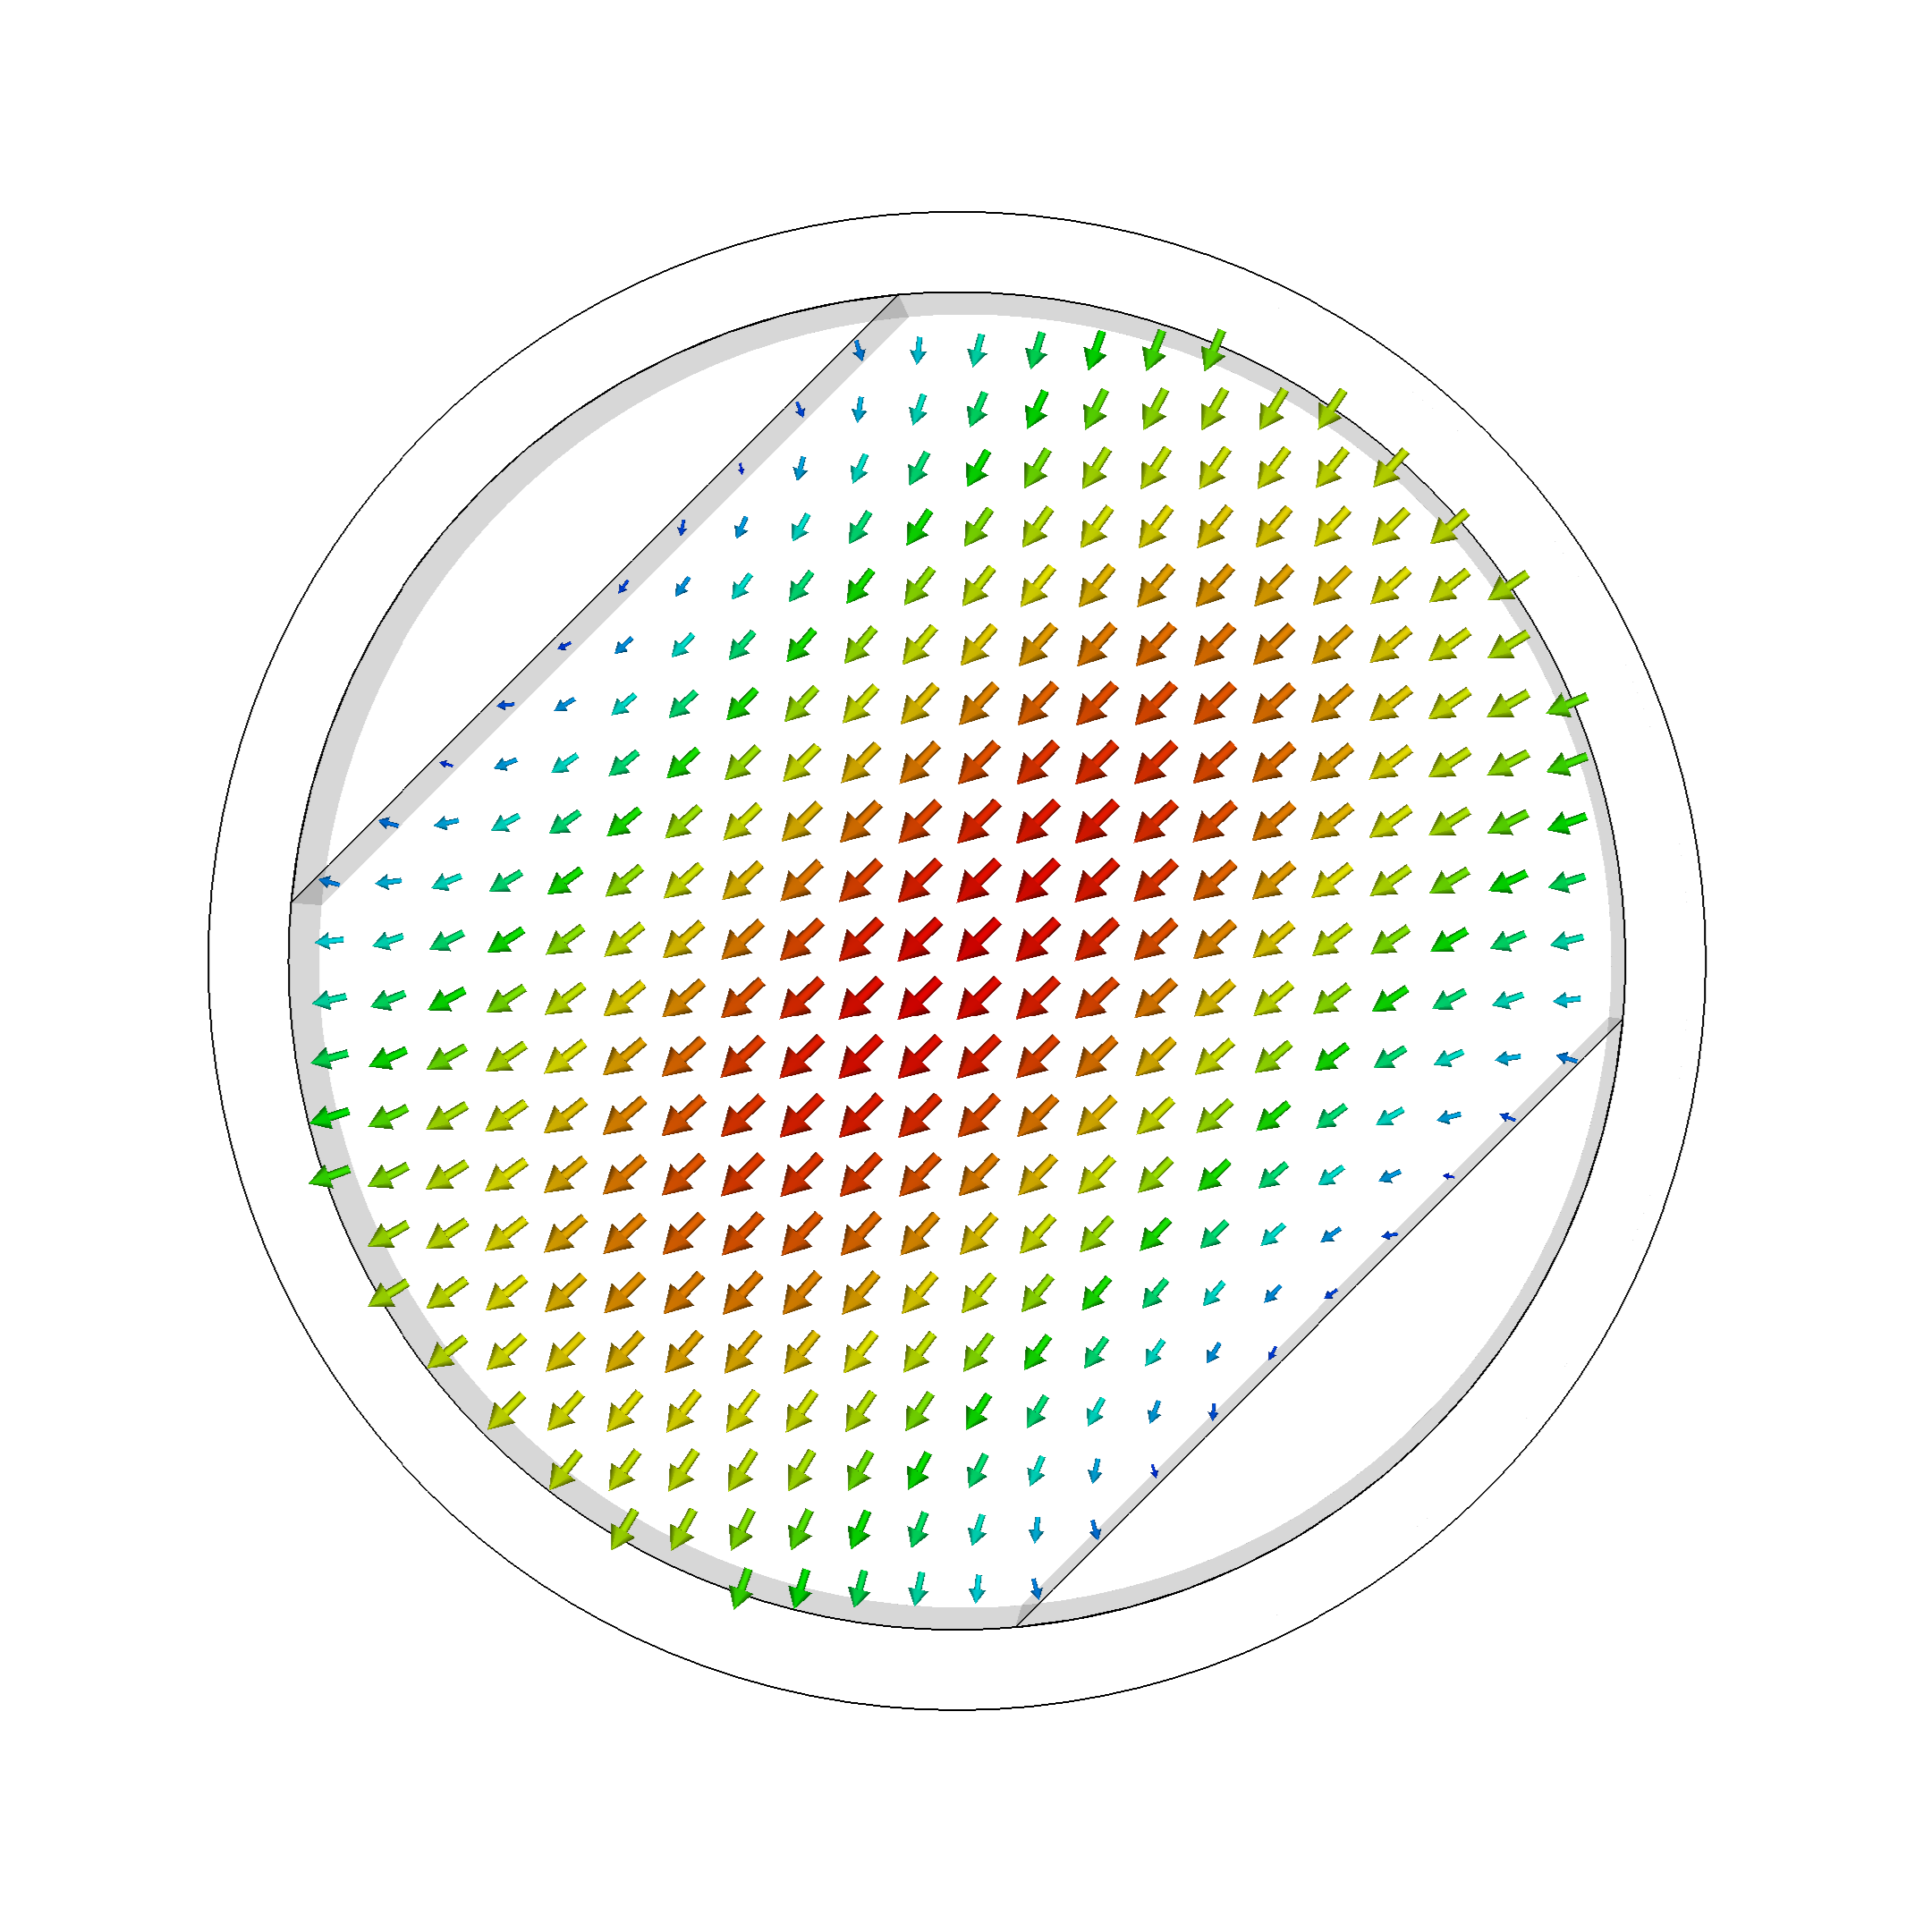
\includegraphics[width=.75\textwidth]{src/polarizer_circular_mode2.png}
        \caption{\label{fig:circular-polarizer-mode2}}
    \end{subfigure}
    \caption{\label{fig:symmetric-polarizer-modes}Fundamental modes of the symmetric waveguides with metallic inserts}
\end{figure}

With the basic modes established, the eigenmodes of the polarizers, i.e., the same waveguides but now \emph{with} the prisms inserted, are analysed. The eigenmodes take the form presented in \cref{fig:square-polarizer-mode1,fig:square-polarizer-mode2} for the square geometry, whereas the circular waveguide with inserts supports two fundamental modes depicted in \cref{fig:circular-polarizer-mode1,fig:circular-polarizer-mode2}. As expected, in both cases, the transverse field exhibits a standing wave behaviour as dictated by the boundary conditions on a conductive surface. More importantly for the polarization transformation, the prisms perturb the electromagnetic fields, leading to a change in the propagation constants of the existing modes. Crucially, the presence of these inserts breaks the original symmetry of the waveguide, causing a dispersion, or difference in phase velocity, between the two fundamental modes of propagation. This fact is illustrated in \cref{fig:symmetric-polarizer-modes}, where in both geometries, one of the modes perceives a different electric path than the other. This dispersion is the key mechanism for achieving circular polarization. As the electromagnetic wave propagates along the waveguide, the phase difference between the two fundamental modes accumulates. By carefully selecting the geometry and placement of the inserts, as well as the length of the waveguide, this cumulative phase lag can be precisely controlled. In the context of a polarizer designed to generate circular polarization, the goal is to achieve exactly one-quarter wavelength phase difference between the two modes at the output. As shown in \cref{eq:polarization-circular-condition}, this quadrature phase relationship, combined with equal amplitudes of the two modes, results in the generation of a circularly polarized wave. The eigenmode analysis allows for the accurate determination of the modal field distributions, enabling precise design and optimization of the polarizer to achieve the desired phase shift and polarization state.

\begin{remark}[Dual polarization capability]
    \label{remark:dual-polarization-capatibility}
    It is important to note that, with respect to the diagonal symmetry of the polarizer, one of its eigenmodes is always antisymmetric. This means that if exciting the square-waveguide-based polarizer with the $\TE 01$ results in a RHCP, the $\TE 10$ must result in LHCP, or vice versa. This principle can be visualized as decomposing the incident waves from \cref{fig:square-waveguide-mode1,fig:square-waveguide-mode2} into the basis formed by polarizer eigenmodes depicted in \cref{fig:square-polarizer-mode1,fig:circular-polarizer-mode2}: While the horizontal waveguide mode (\cref{fig:square-waveguide-mode1}) can be expressed as a simple sum of the two polarizer modes, the vertical waveguide mode (\cref{fig:square-waveguide-mode2}) requires the negative%
        \footnote{A positive sum of the two eigenmodes is equivalent to the plus sign option in \cref{eq:polarization-circular-e-r0}, as the condition on circular polarization expressed in \cref{eq:polarization-circular-condition} is fulfilled due to the two eigenmodes oscillating perpendicular to each other, i.e., $\delta = \pi/2$. Conversely, adding one eigenmode to the negative of the other introduces an additional $\pi$ to the phase difference $\delta$. The condition for circular polarization is again fulfilled, but with $\delta = 3\pi/2$, causing the sine in \cref{eq:polarization-circular-e-r0} to take a negative value, resulting in the opposite circular polarization.}
    of the antisymmetric polarizer mode (\cref{fig:square-polarizer-mode2}). Although this principle was illustrated using the square waveguide structure, the same holds true for the circular geometry with its two orthogonal degenerate modes (\cref{fig:circular-waveguide-mode1,fig:circular-waveguide-mode2}). This unique property enables the structures to produce dual circular polarization simply by switching between two excitations.

    Furthermore, due to the mirror symmetry of both polarizers, optimizing the structure with respect to just a single orientation of circular polarization is sufficient. By the essence of the matter, the other polarization must retain the same performance parameters, as will be proven by simulation.
\end{remark}

\subsection{Figures of merit}
A crucial outcome of the eigenmode analysis is the gained insight into the operational principles, which helps define relevant variables and performance parameters intrinsic to the structure's geometry, ultimately aiding in polarizer optimization. The optimization process aims to produce circular polarization while minimizing production costs, primarily by reducing the polarizer length, $L$. This necessitates maximizing the \emph{specific mode phase shift}, given by
\begin{align}
    \label{eq:polarizer-specific-phase-shift}
    \Delta k_L(f) &= \frac 1L \int_0^L \[k_2-k_1\](z,f)\,\d z,
\end{align}
where $k_1$ and $k_2$ are the propagation constants of the two polarizer modes and $z$ is the Cartesian coordinate aligned with the propagation direction. This quantity represents the average difference in propagation constants between the two modes along the polarizer,%
    \footnote{This quantity is analogous to the birefringence effect observed in optics, where a material exhibits different refractive indices for different polarizations, causing a phase difference to accumulate between them as they propagate. Here, the waveguide structure, due to its geometry, effectively creates different propagation constants for the two orthogonal modes, leading to a similar effect.}
effectively quantifying the rate at which the phase difference between them accumulates as they propagate. However, \cref{eq:polarizer-specific-phase-shift} addresses only one of the two conditions for circular polarization \eqref{eq:polarization-circular-condition}, the other being the requirement for equal mode amplitudes:
\begin{align}
    \label{eq:polarizer-amplitude-ratio}
    \left.\frac{E_2}{E_1}\right|_{z=L} = 1,
\end{align}
where $E_1$ and $E_2$ are the amplitudes of the two modes and the polarizer output. A weighted aggregate of \cref{eq:polarizer-specific-phase-shift,eq:polarizer-amplitude-ratio} forms the objective function of the optimization problem, with the variables being the geometric parameters of the polarizer cross-section. Intuitively, larger inserted prisms induce a greater phase lag per unit length but also introduce larger amplitude distortions between the modes. This reveals an inherent conflict within the problem, necessitating a trade-off. From an application perspective, a balance must be struck between the length of the structure, which compensates for a lower phase delay per unit length, and polarization purity, which is compromised by unequal mode magnitudes.

Let's draft up some numbers for the geometries and compare the polarizer geometries. Also simplify \cref{eq:polarizer-specific-phase-shift} and talk about how we extract both metrics in CST.

\subsection{Comparison of symmetric waveguides}
To conclude the eigenmode analysis, a determination will be made, using the previously introduced figures of merit, regarding which geometry is better suited for polarization control, considering both practical and performance aspects. Ideally, minimal frequency dependence of both figures, \cref{eq:polarizer-specific-phase-shift,eq:polarizer-amplitude-ratio}, is desired. However, due to the inherently resonant operational principle of the waveguide, achieving feasible performance across an ultrawide band with a single section of such a polarizing structure is not considered possible.

Before proceeding, the practical evaluation of \cref{eq:polarizer-specific-phase-shift,eq:polarizer-amplitude-ratio}  should be addressed. Given that both polarizers are analysed as uniform waveguides (\cref{fig:polarizer-square-perspective,fig:polarizer-circular-perspective}), the propagation dispersion between the two modes, and consequently both metrics, can be approximated as constant throughout the polarizer. This approximation allows \cref{eq:polarizer-specific-phase-shift} to be expressed as
\begin{align}
    \label{eq:polarizer-phase-shift}
    \Delta k_L(f) &= \[k_2-k_1\](f)
\end{align}
and the overall mode phase shift at the polarizer output is given by
\begin{align}
    \Delta\phi(f) &= L\[k_2-k_1\](f).
\end{align}

Furthermore, this simplification permits the evaluation of both \cref{eq:polarizer-amplitude-ratio,eq:polarizer-phase-shift} from a single reading at the polarizer output. For this purpose, an \emph{E-field probe} functionality within CST Studio Suite can be utilized, allowing the magnitude and phase of the electric field to be determined at a specified point in space, evaluated across all frequencies. Consequently, the objective function for maximum specific phase shift, \cref{eq:polarizer-specific-phase-shift}, is transformed into the minimization of
\begin{align}
    L_\perp(f) &= \frac\pi4\frac{L}{\Delta\phi}(f)
\end{align}
representing the polarizer length required to achieve a mode phase shift of $\pi/4$.%
    \footnote{It is important to note that, due to phase wrapping, the cross-section tuning simulations must be
    conducted for a polarizer shorter than that required to produce a $\pi/4$ phase shift.}
This modified objective function can be readily computed using the \emph{Template-Based Post-Processing} feature within CST Studio Suite, using $\Delta\phi(f)$ obtained from the E-field probe result. Moreover, the practical feasibility of the polarizer is inherently incorporated into this formulation.

\begin{figure}[!ht]
    \centering
    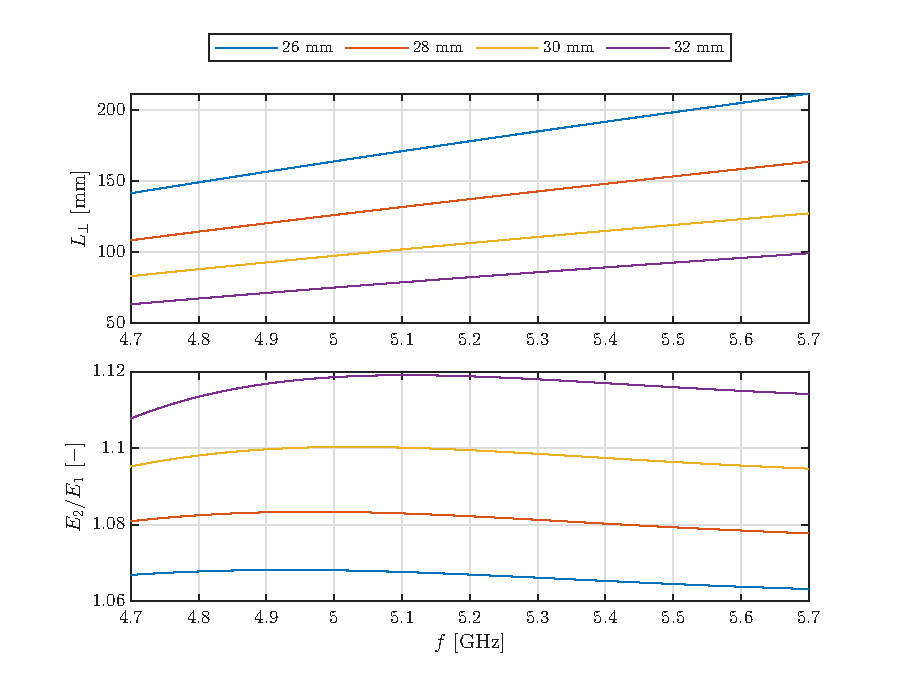
\includegraphics[width=\textwidth]{src/circular_polarizer_cross_section.eps}
    \caption{\label{fig:circular-polarizer-cross-section}Circular polarizer cross-section}
\end{figure}

\begin{figure}[!ht]
    \centering
    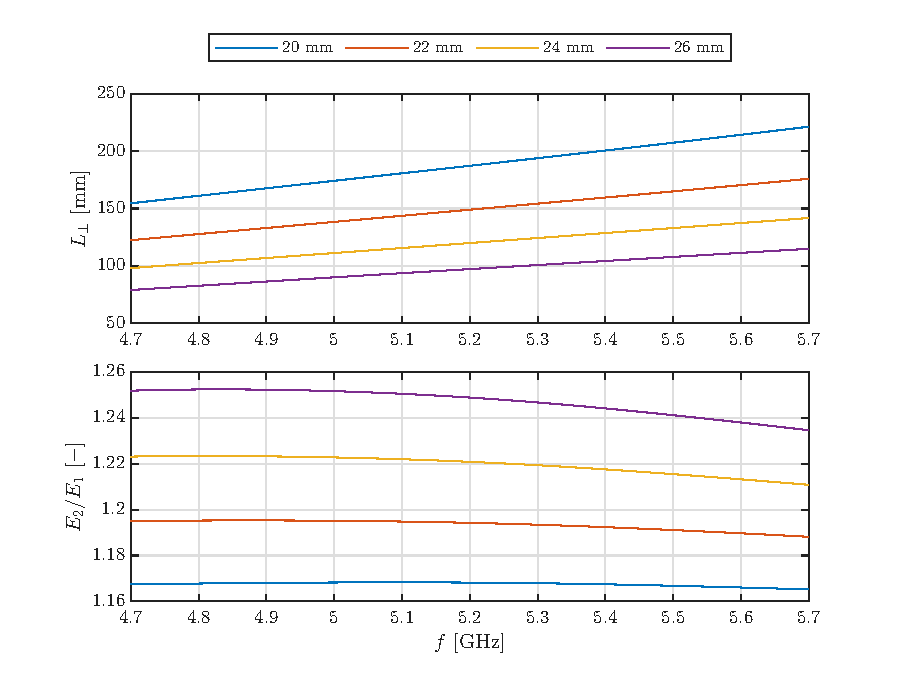
\includegraphics[width=\textwidth]{src/square_polarizer_cross_section.eps}
    \caption{\label{fig:square-polarizer-cross-section}Square polarizer cross-section}
\end{figure}

\begin{figure}[!ht]
    \centering
    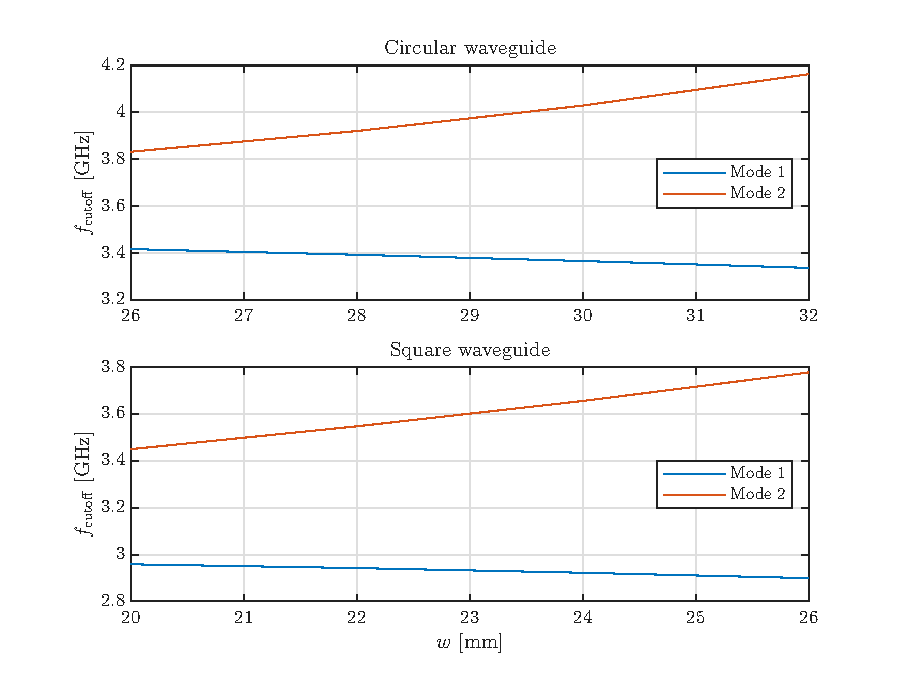
\includegraphics[width=\textwidth]{src/polarizers_cutoff_frequencies.eps}
    \caption{\label{fig:polarizers-cutoff-frequencies}Polarizers -- cutoff frequencies}
\end{figure}

\section{Square waveguide polarizer}

\subsection{Selection of parameters}
Frequency band, reference commercial waveguide for recommended band, side length determination, polarizer length determination, \dots

\subsection{Cross-section tuning}
Trade-off: unit mode amplitude ratio vs. high mode phase lag per unit length, \dots

\section{Simulation results}
Add text, \dots

\subsection{Waveguide feed simulation}
Exciting the structure with a waveguide feed with two modes, mode metrics \dots

\subsection{Radiation properties}
Using open-ended waveguide, \dots

\chapter{Feeding structure}
\label{chapter:feeding-structure}

\section{Coaxial-to-waveguide transition}
Single feed, dual feed from \parencite{karki-et-al:dual-polarized-probe-for-planar-near-field-measurement}, \dots

\section{Dual feed}
Add text, \dots

\subsection{Single feed}
Right-angle transition, simulation boundary consideration, effects of individual parameters, optimization, \dots

\subsection{Grating}
Isolation of optimization variables, reflection vs. cross-talk minimization trade-off, \dots

\subsection{Dual feed optimization}
Initial results, optimization script, \dots

\chapter{Antenna}
\label{chapter:antenna}
Add text including target gain

\section{Conical horn}
Theoretical guidelines from \parencite{aboserwal-et-al:conical-horn-gain-and-amplitude-patterns}, Antenna Magus, adaptation of a conical horn to a square waveguide \dots

\section{Simulation results}
Design using Antenna Magus, effects of individual parameters when adapting the geometry, \dots

\newpage
\chapter{Assembly}
\label{chapter:assembly}
Add text, \dots

\section{First results}
The tragic results, analysis, \dots

\section{Grating removal}
Decision reasoning, lack of grating's meaning, \dots

\section{Product finalization}
Tuning results vs. optimization, fine-mesh and high-precision verifications, practical assembly adjustments by UMT, \dots

\section{Measurement results}
Comparison of measurement results with simulation data, \dots

%========== Conclusion ==========
\chapter*{Conclusion}
\label{chap:conclusion}
\addcontentsline{toc}{chapter}{\nameref{chap:conclusion}}

\lipsum[10-13]

%========== Nomenclature ==========
\printnomenclature

%========== Bibliography ==========
\printbibliography[heading=bibintoc]

% %========== Index ==========
\printindex

\end{document}
